% Generated by thesis/ch7/exp2/networks.py -- do not edit by hand.
% Appendix: the 30 Experiment 2 networks, as trained and as explained (60 figures).
% Adult: the ten networks (the dataset is named in each caption)
% Generated by thesis/ch7/exp2/networks.py -- do not edit by hand.
\begin{sidewaysfigure}
  \centering
  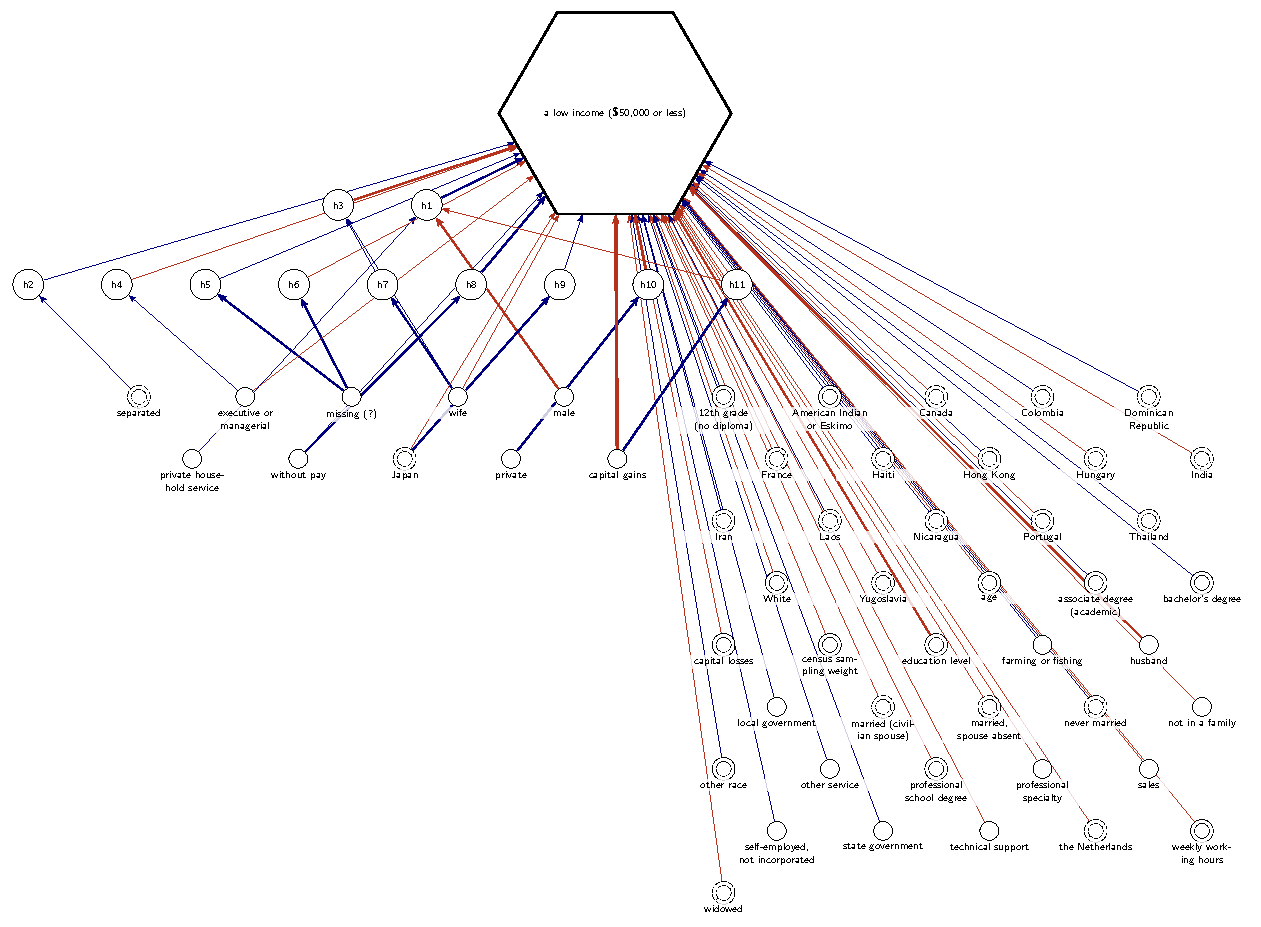
\includegraphics[width=\textheight,height=0.78\textwidth,keepaspectratio]{figures/exp2/networks/adult-s0-raw}
  \caption{Adult, seed 0 (adult-s0): the network as trained, before any explanation, in full. Inputs at the bottom (every input column its own node), hidden units by depth, the output at the top; 51 of 107 input columns are connected, with 11 hidden units and 70 enabled connections. Blue: positive weight (raises the score); red: negative weight (lowers it); thicker: larger weight. Orange outline and up arrow: raises the final prediction; teal and down arrow: lowers it; grey and double arrow: depends. Not used (no connection; 56 columns): federal government, never worked, self-employed, incorporated, 10th grade, 11th grade, doctorate, high-school graduate, master's degree, preschool, some college, 1st-4th grade, 5th-6th grade, 7th-8th grade, 9th grade, associate degree (vocational), divorced, married to a member of the armed forces, missing (?), administrative or clerical, protective service, transport or moving, armed forces, craft or repair, handlers or cleaners, machine operator or inspector, other relative, own child, unmarried, Asian or Pacific Islander, Black, missing (?), Cambodia, Germany, Greece, Guatemala, Honduras, Ireland, Italy, Jamaica, Mexico, outlying US territories (Guam, US Virgin Islands), Peru, China, the Philippines, Poland, Puerto Rico, Scotland, 'South' (as recorded), Taiwan, Trinidad and Tobago, the United States, Vietnam, Cuba, Ecuador, El Salvador and England.}
  \label{fig:exp2-net-adult-s0-raw}
\end{sidewaysfigure}

\clearpage
% Generated by thesis/ch7/exp2/networks.py -- do not edit by hand.
\begin{sidewaysfigure}
  \centering
  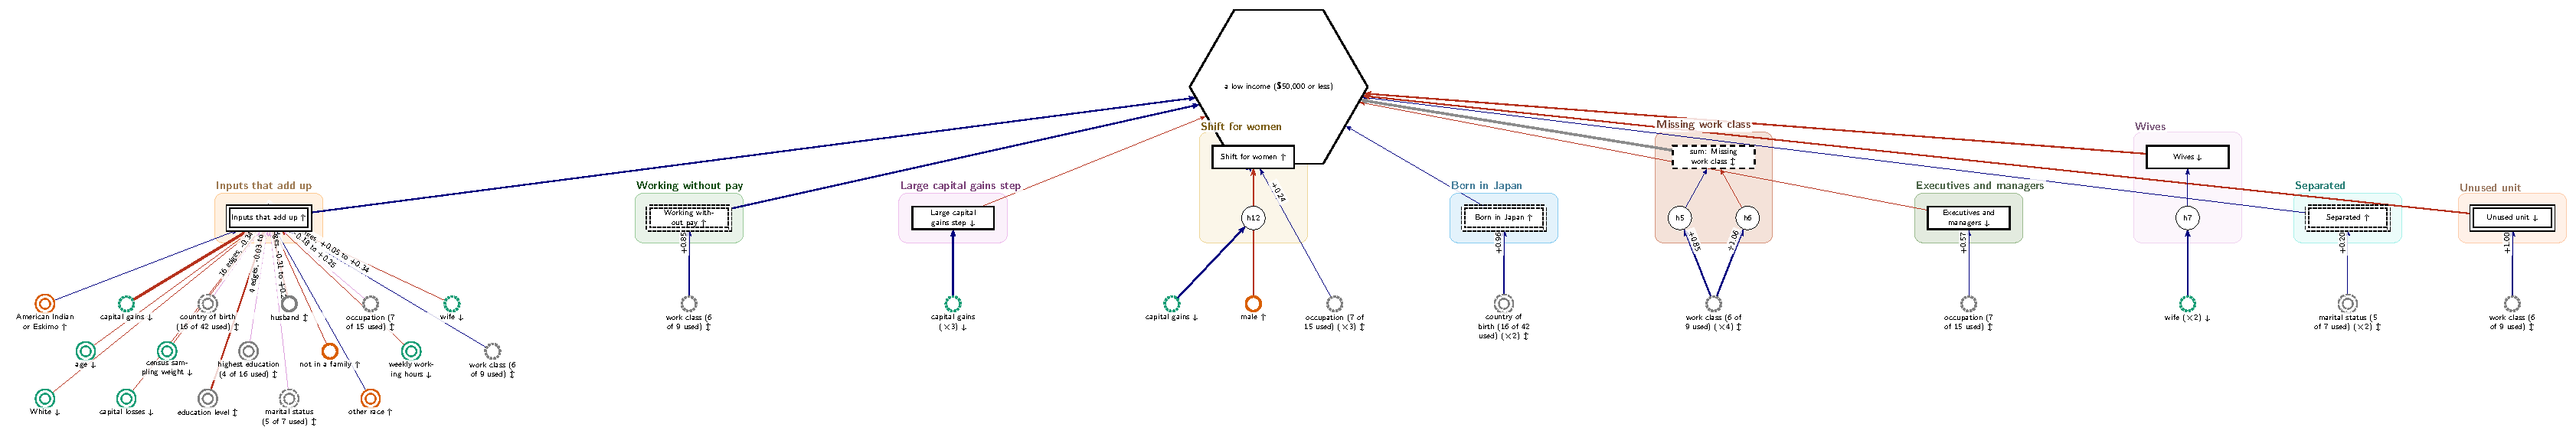
\includegraphics[width=\textheight,height=0.9\textwidth,keepaspectratio]{figures/exp2/networks/adult-s0-explained}
  \caption{Adult, seed 0: the explained network, every unit nested by part.}
  \label{fig:exp2-net-adult-s0-explained}
\end{sidewaysfigure}

\clearpage
% Generated by thesis/ch7/exp2/networks.py -- do not edit by hand.
\begin{sidewaysfigure}
  \centering
  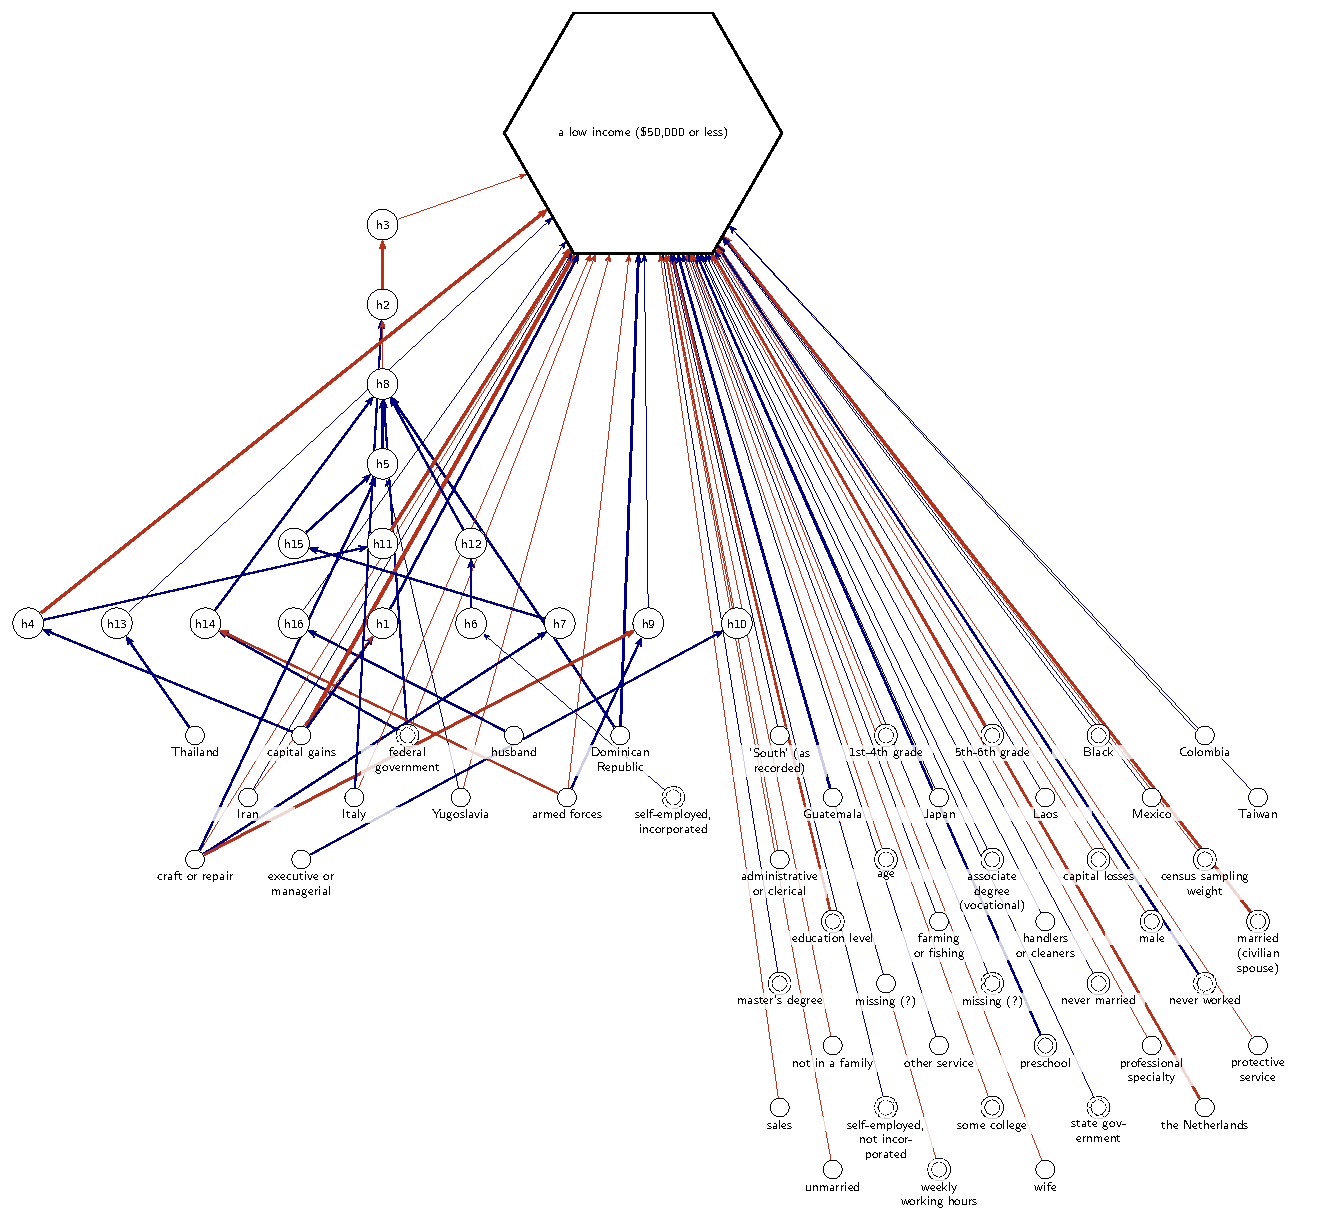
\includegraphics[width=\textheight,height=0.78\textwidth,keepaspectratio]{figures/exp2/networks/adult-s1-raw}
  \caption{Adult, seed 1 (adult-s1): the network as trained, before any explanation, in full. Inputs at the bottom (every input column its own node), hidden units by depth, the output at the top; 50 of 107 input columns are connected, with 16 hidden units and 80 enabled connections. Blue: positive weight (raises the score); red: negative weight (lowers it); thicker: larger weight. Orange outline and up arrow: raises the final prediction; teal and down arrow: lowers it; grey and double arrow: depends. Not used (no connection; 57 columns): local government, private, without pay, 10th grade, 11th grade, doctorate, high-school graduate, professional school degree, 12th grade (no diploma), 7th-8th grade, 9th grade, associate degree (academic), bachelor's degree, divorced, married to a member of the armed forces, married, spouse absent, separated, widowed, missing (?), technical support, transport or moving, machine operator or inspector, private household service, other relative, own child, American Indian or Eskimo, Asian or Pacific Islander, other race, White, Cambodia, France, Germany, Greece, Haiti, Honduras, Hong Kong, Hungary, India, Canada, Ireland, Jamaica, Nicaragua, outlying US territories (Guam, US Virgin Islands), Peru, China, the Philippines, Poland, Portugal, Puerto Rico, Scotland, Trinidad and Tobago, the United States, Vietnam, Cuba, Ecuador, El Salvador and England.}
  \label{fig:exp2-net-adult-s1-raw}
\end{sidewaysfigure}

\clearpage
% Generated by thesis/ch7/exp2/networks.py -- do not edit by hand.
\begin{sidewaysfigure}
  \centering
  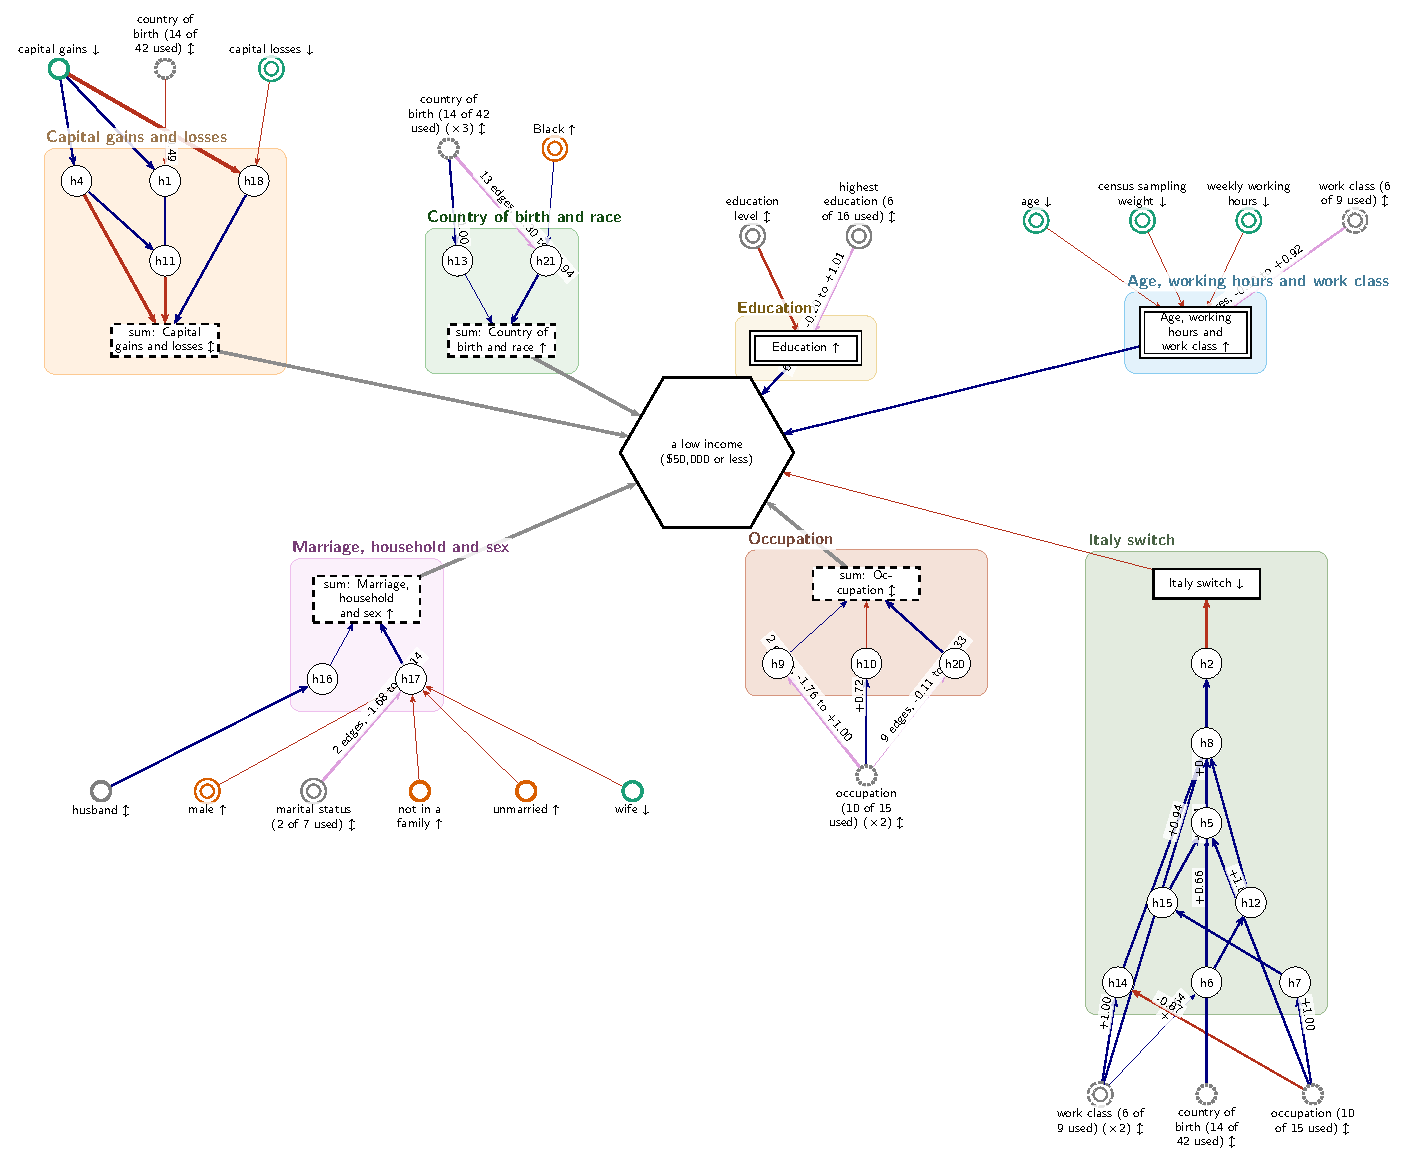
\includegraphics[width=\textheight,height=0.9\textwidth,keepaspectratio]{figures/exp2/networks/adult-s1-explained}
  \caption{Adult, seed 1: the explained network, every unit nested by part.}
  \label{fig:exp2-net-adult-s1-explained}
\end{sidewaysfigure}

\clearpage
% Generated by thesis/ch7/exp2/networks.py -- do not edit by hand.
\begin{sidewaysfigure}
  \centering
  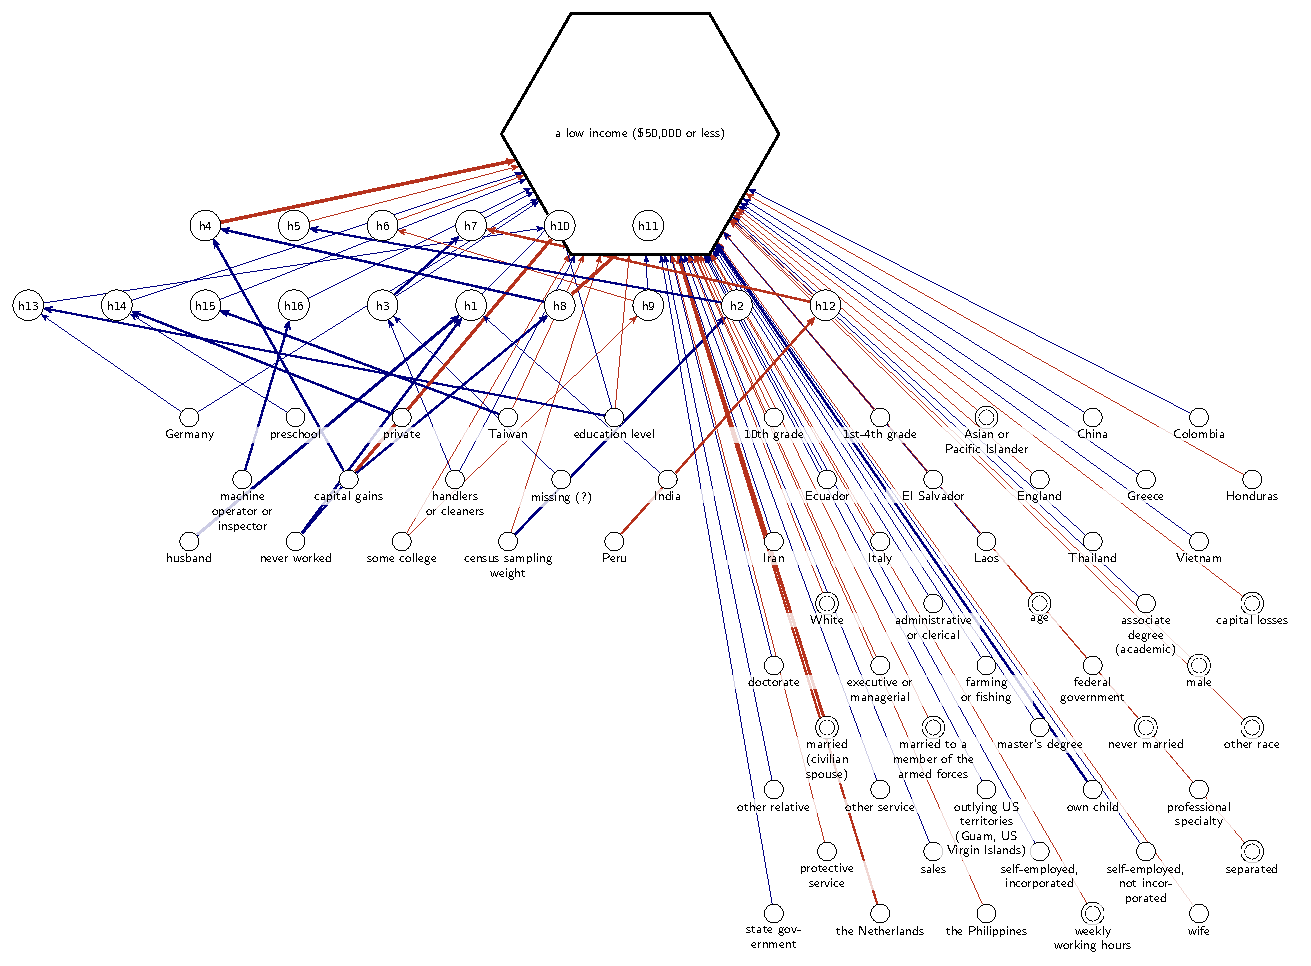
\includegraphics[width=\textheight,height=0.78\textwidth,keepaspectratio]{figures/exp2/networks/adult-s2-raw}
  \caption{Adult, seed 2 (adult-s2): the network as trained, before any explanation, in full. Inputs at the bottom (every input column its own node), hidden units by depth, the output at the top; 60 of 107 input columns are connected, with 16 hidden units and 91 enabled connections. Blue: positive weight (raises the score); red: negative weight (lowers it); thicker: larger weight. Orange outline and up arrow: raises the final prediction; teal and down arrow: lowers it; grey and double arrow: depends. Not used (no connection; 47 columns): missing (?), local government, without pay, 11th grade, high-school graduate, professional school degree, 12th grade (no diploma), 5th-6th grade, 7th-8th grade, 9th grade, associate degree (vocational), bachelor's degree, divorced, married, spouse absent, widowed, technical support, transport or moving, armed forces, craft or repair, private household service, not in a family, unmarried, American Indian or Eskimo, Black, missing (?), Cambodia, France, Guatemala, Haiti, Hong Kong, Hungary, Canada, Ireland, Jamaica, Japan, Mexico, Nicaragua, Poland, Portugal, Puerto Rico, Scotland, 'South' (as recorded), Trinidad and Tobago, the United States, Yugoslavia, Cuba and Dominican Republic.}
  \label{fig:exp2-net-adult-s2-raw}
\end{sidewaysfigure}

\clearpage
% Generated by thesis/ch7/exp2/networks.py -- do not edit by hand.
\begin{sidewaysfigure}
  \centering
  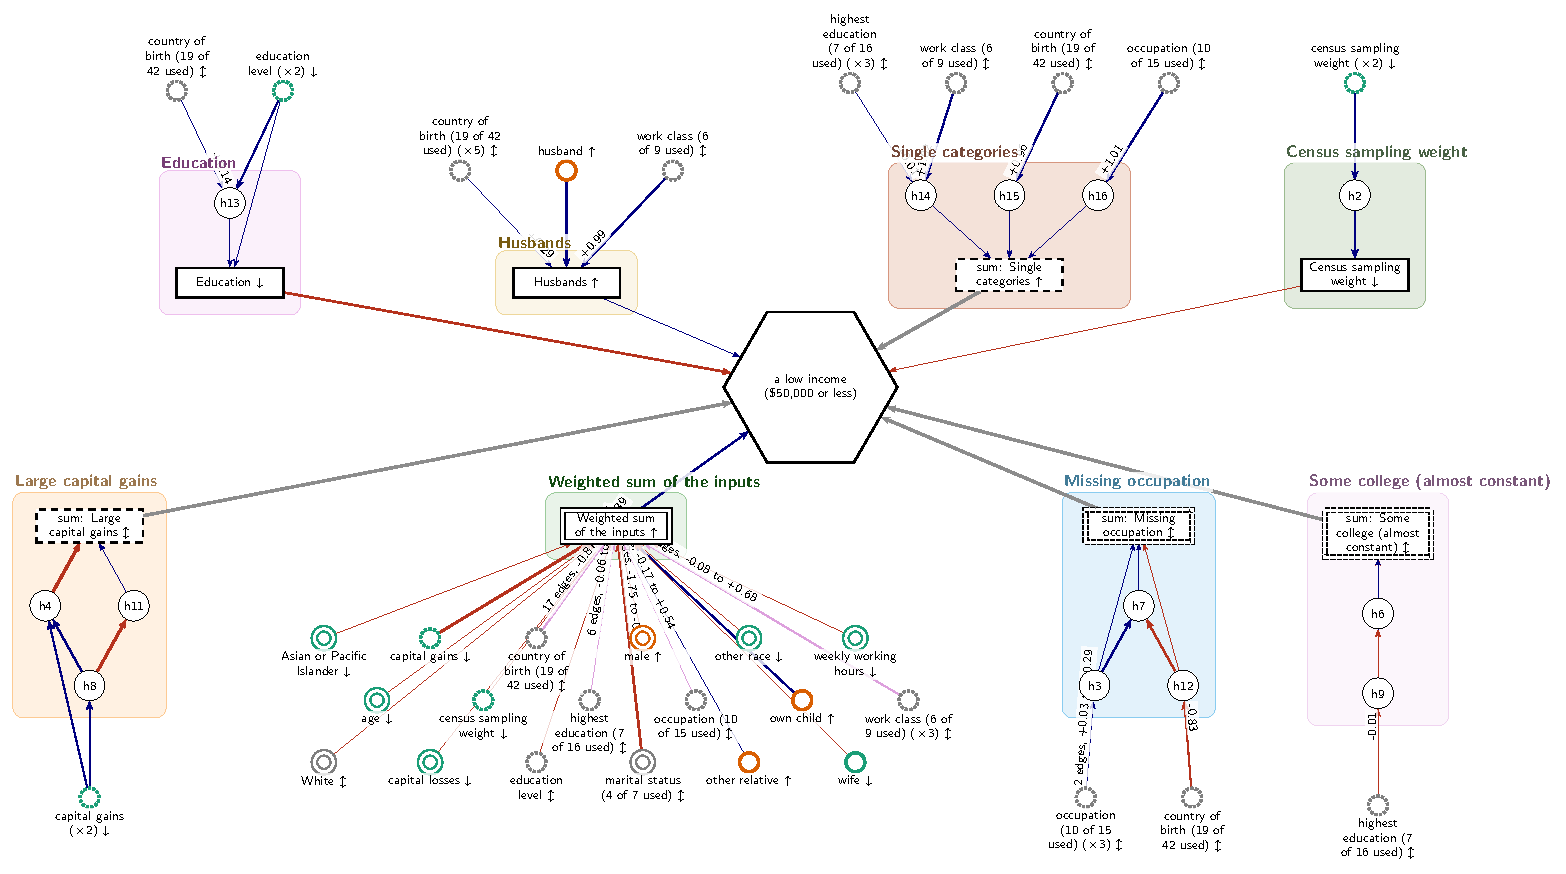
\includegraphics[width=\textheight,height=0.78\textwidth,keepaspectratio]{figures/exp2/networks/adult-s2-explained}
  \caption{Adult, seed 2 (adult-s2): every unit and connection of the explained model, nested by part. Shaded clusters are the 9 parts of the agent's explanation (8 leaf and 1 composition annotations, after 9 node splits and 1 identity nodes) and darker boxes the parts inside them; circles are hidden units; each cluster's rectangle is its output, a dashed `sum' an addition the next unit does; the hexagon is the model's output. An input used by several parts is drawn under each of them (dotted outline). Blue: positive weight (raises the score); red: negative weight (lowers it); thicker: larger weight. Orange outline and up arrow: raises the final prediction; teal and down arrow: lowers it; grey and double arrow: depends.}
  \label{fig:exp2-net-adult-s2-explained}
\end{sidewaysfigure}

\clearpage
% Generated by thesis/ch7/exp2/networks.py -- do not edit by hand.
\begin{sidewaysfigure}
  \centering
  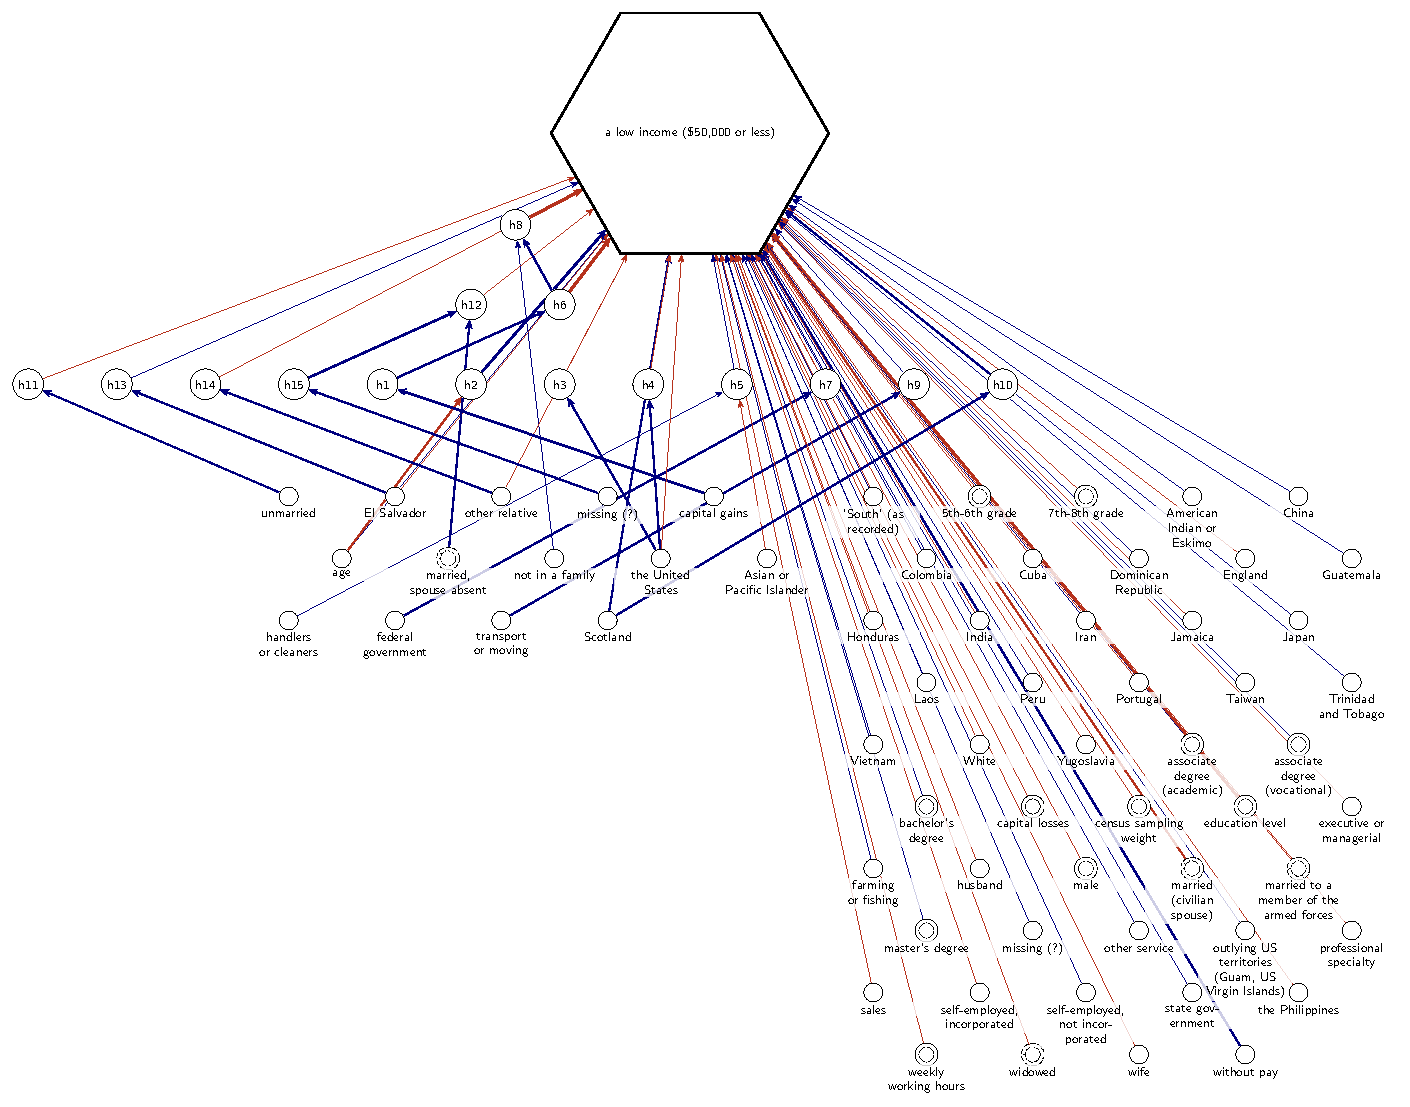
\includegraphics[width=\textheight,height=0.78\textwidth,keepaspectratio]{figures/exp2/networks/adult-s3-raw}
  \caption{Adult, seed 3 (adult-s3): the network as trained, before any explanation, in full. Inputs at the bottom (every input column its own node), hidden units by depth, the output at the top; 63 of 107 input columns are connected, with 15 hidden units and 85 enabled connections. Blue: positive weight (raises the score); red: negative weight (lowers it); thicker: larger weight. Orange outline and up arrow: raises the final prediction; teal and down arrow: lowers it; grey and double arrow: depends. Not used (no connection; 44 columns): missing (?), local government, never worked, private, 10th grade, 11th grade, doctorate, high-school graduate, preschool, professional school degree, some college, 12th grade (no diploma), 1st-4th grade, 9th grade, divorced, never married, separated, administrative or clerical, protective service, technical support, armed forces, craft or repair, machine operator or inspector, private household service, own child, Black, other race, Cambodia, France, Germany, Greece, Haiti, the Netherlands, Hong Kong, Hungary, Canada, Ireland, Italy, Mexico, Nicaragua, Poland, Puerto Rico, Thailand and Ecuador.}
  \label{fig:exp2-net-adult-s3-raw}
\end{sidewaysfigure}

\clearpage
% Generated by thesis/ch7/exp2/networks.py -- do not edit by hand.
\begin{sidewaysfigure}
  \centering
  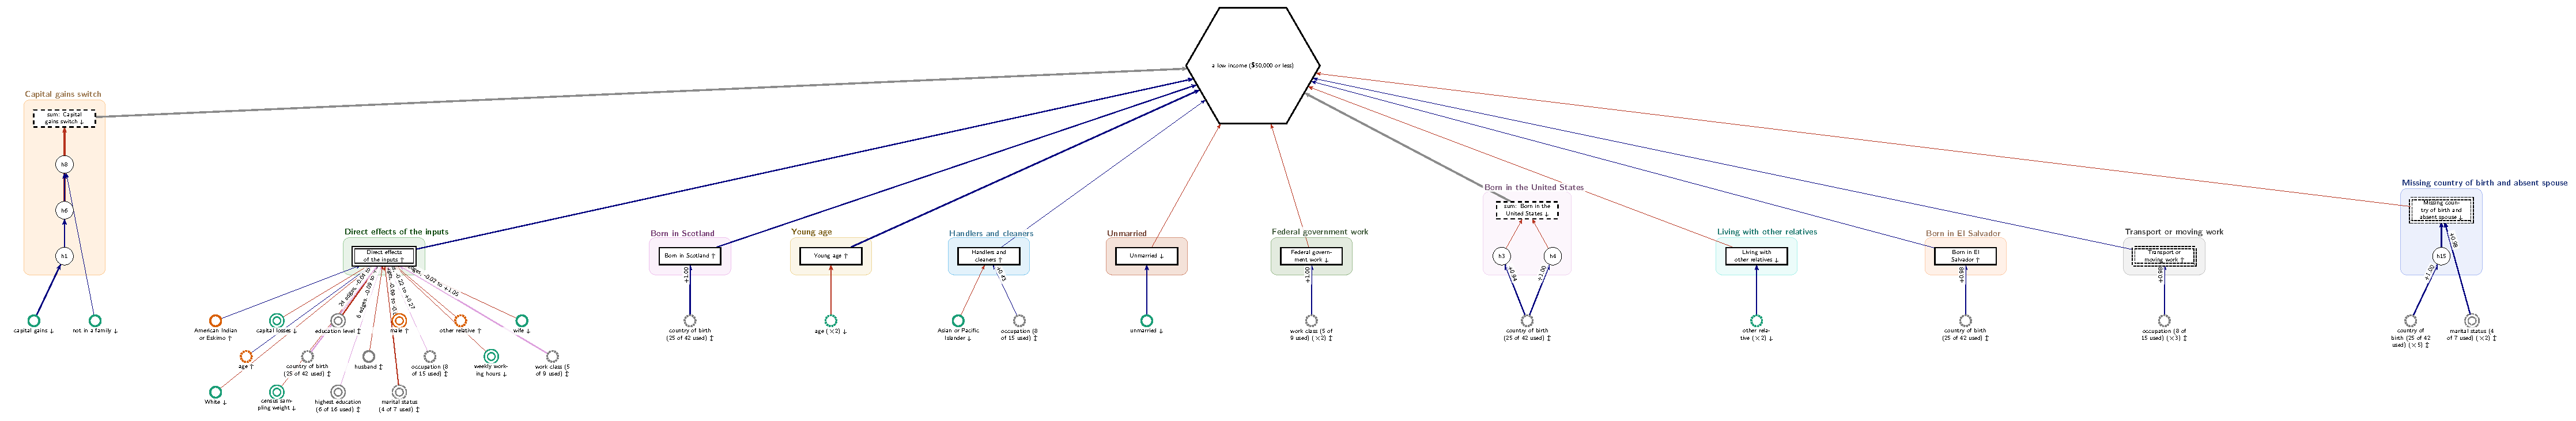
\includegraphics[width=\textheight,height=0.78\textwidth,keepaspectratio]{figures/exp2/networks/adult-s3-explained}
  \caption{Adult, seed 3 (adult-s3): every unit and connection of the explained model, nested by part. Shaded clusters are the 13 parts of the agent's explanation (12 leaf and 1 composition annotations, after 5 node splits and 1 identity nodes) and darker boxes the parts inside them; circles are hidden units; each cluster's rectangle is its output, a dashed `sum' an addition the next unit does; the hexagon is the model's output. An input used by several parts is drawn under each of them (dotted outline). Blue: positive weight (raises the score); red: negative weight (lowers it); thicker: larger weight. Orange outline and up arrow: raises the final prediction; teal and down arrow: lowers it; grey and double arrow: depends.}
  \label{fig:exp2-net-adult-s3-explained}
\end{sidewaysfigure}

\clearpage
% Generated by thesis/ch7/exp2/networks.py -- do not edit by hand.
\begin{sidewaysfigure}
  \centering
  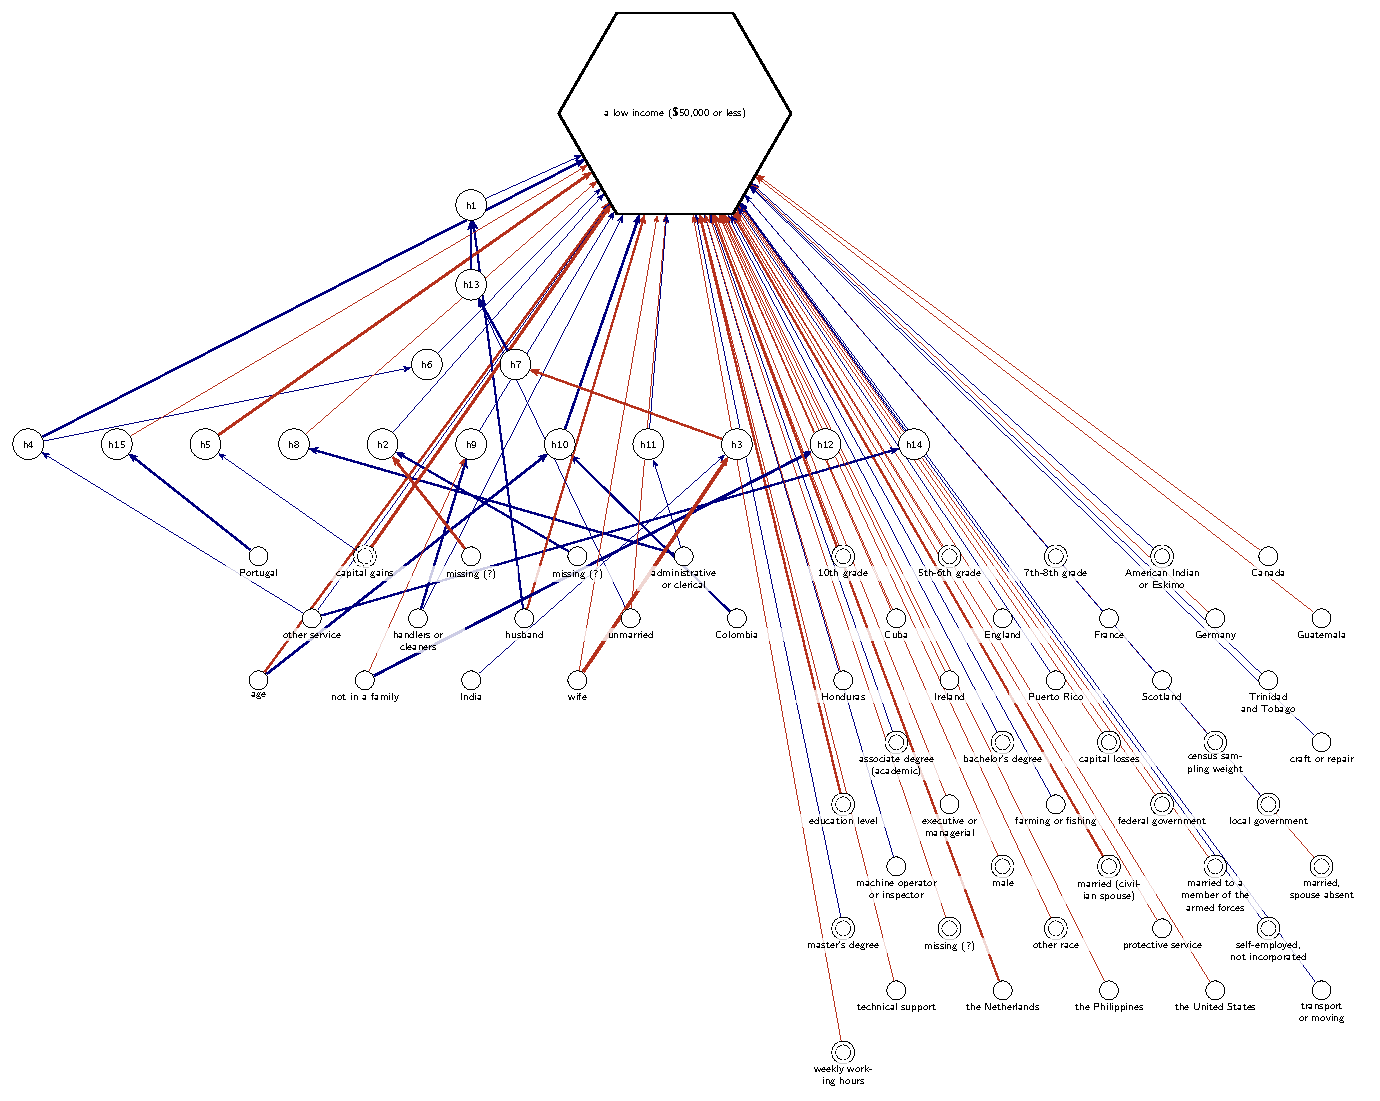
\includegraphics[width=\textheight,height=0.78\textwidth,keepaspectratio]{figures/exp2/networks/adult-s4-raw}
  \caption{Adult, seed 4 (adult-s4): the network as trained, before any explanation, in full. Inputs at the bottom (every input column its own node), hidden units by depth, the output at the top; 55 of 107 input columns are connected, with 15 hidden units and 81 enabled connections. Blue: positive weight (raises the score); red: negative weight (lowers it); thicker: larger weight. Orange outline and up arrow: raises the final prediction; teal and down arrow: lowers it; grey and double arrow: depends. Not used (no connection; 52 columns): never worked, private, self-employed, incorporated, state government, without pay, 11th grade, doctorate, high-school graduate, preschool, professional school degree, some college, 12th grade (no diploma), 1st-4th grade, 9th grade, associate degree (vocational), divorced, never married, separated, widowed, professional specialty, sales, armed forces, private household service, other relative, own child, Asian or Pacific Islander, Black, White, Cambodia, Greece, Haiti, Hong Kong, Hungary, Iran, Italy, Jamaica, Japan, Laos, Mexico, Nicaragua, outlying US territories (Guam, US Virgin Islands), Peru, China, Poland, 'South' (as recorded), Taiwan, Thailand, Vietnam, Yugoslavia, Dominican Republic, Ecuador and El Salvador.}
  \label{fig:exp2-net-adult-s4-raw}
\end{sidewaysfigure}

\clearpage
% Generated by thesis/ch7/exp2/networks.py -- do not edit by hand.
\begin{sidewaysfigure}
  \centering
  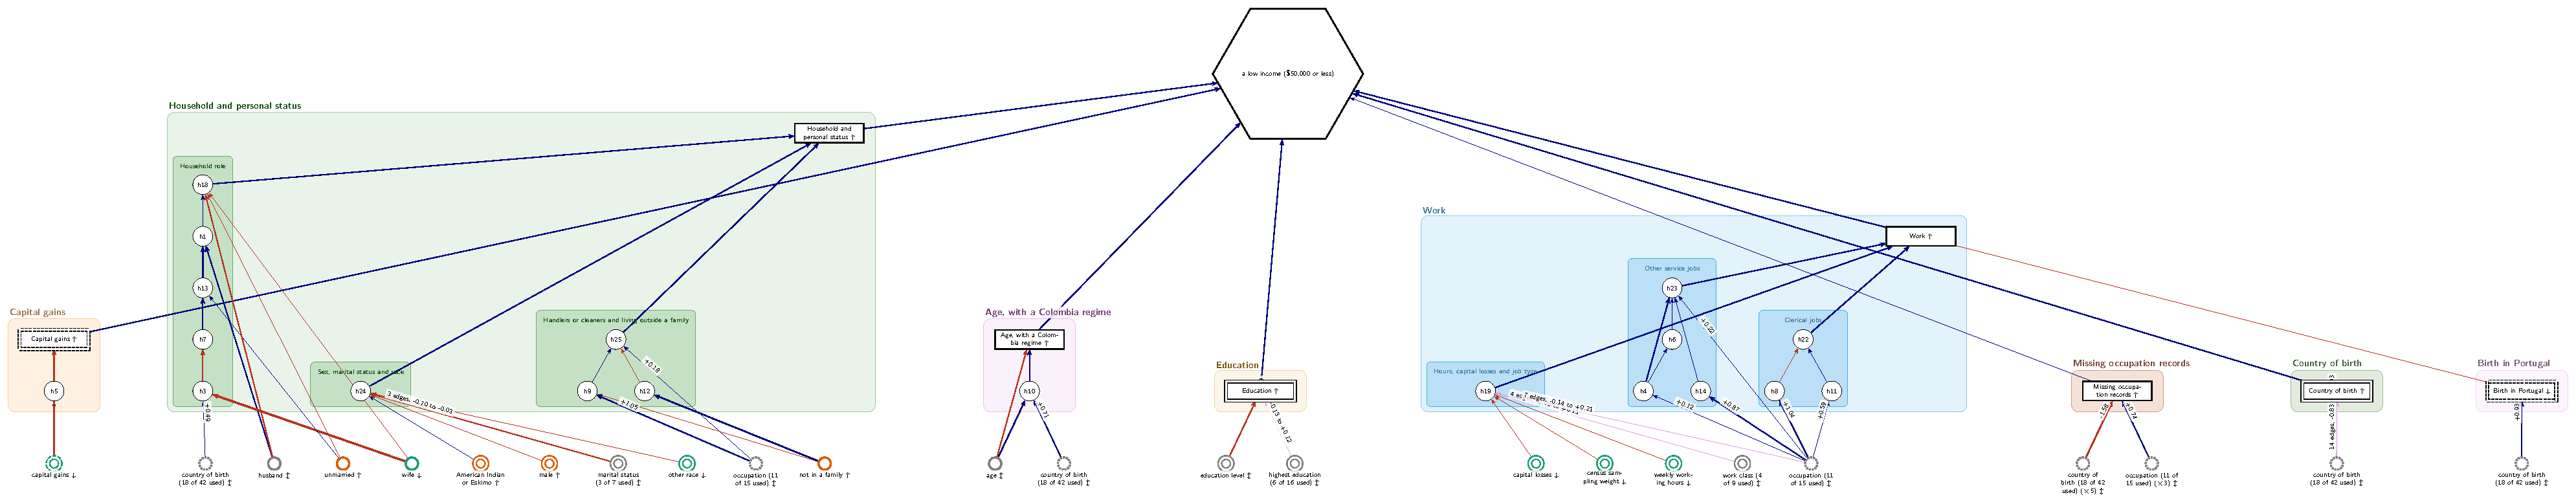
\includegraphics[trim={0.0bp 0 943.2bp 0},clip,width=\textheight,height=0.78\textwidth,keepaspectratio]{figures/exp2/networks/adult-s4-explained}
  \caption{Adult, seed 4 (adult-s4): every unit and connection of the explained model, nested by part. Shaded clusters are the 15 parts of the agent's explanation (12 leaf and 3 composition annotations, after 0 node splits and 12 identity nodes) and darker boxes the parts inside them; circles are hidden units; each cluster's rectangle is its output, a dashed `sum' an addition the next unit does; the hexagon is the model's output. An input used by several parts is drawn under each of them (dotted outline). Blue: positive weight (raises the score); red: negative weight (lowers it); thicker: larger weight. Orange outline and up arrow: raises the final prediction; teal and down arrow: lowers it; grey and double arrow: depends. Drawn in 2 pieces, left to right, on this and the next page.}
  \label{fig:exp2-net-adult-s4-explained}
\end{sidewaysfigure}
\clearpage
\begin{sidewaysfigure}
  \centering
  \ContinuedFloat
  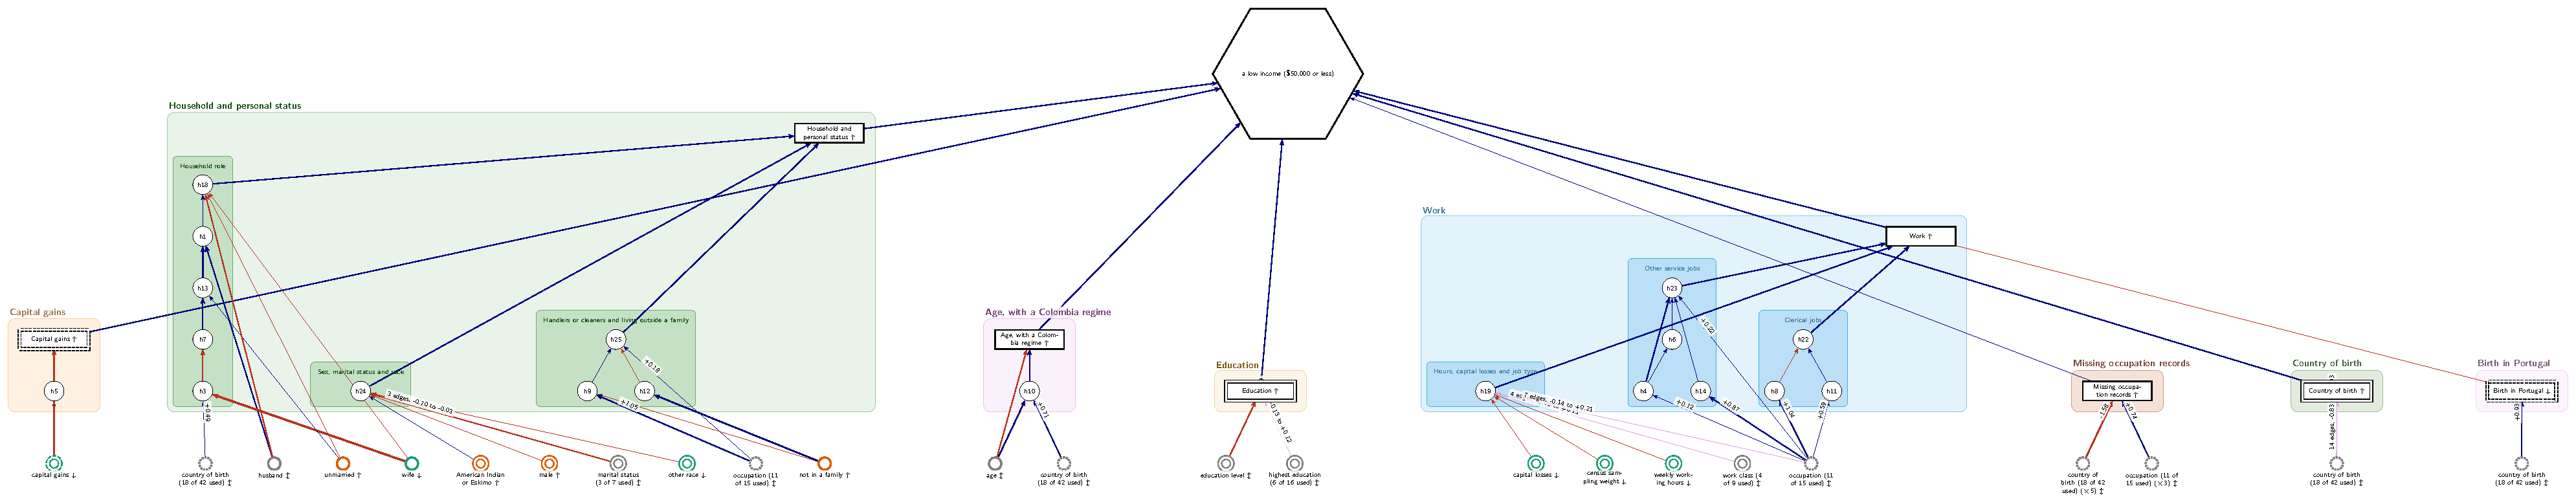
\includegraphics[trim={943.2bp 0 0.0bp 0},clip,width=\textheight,height=0.78\textwidth,keepaspectratio]{figures/exp2/networks/adult-s4-explained}
  \caption[]{(continued, piece 2 of 2).}
\end{sidewaysfigure}

\clearpage
% Generated by thesis/ch7/exp2/networks.py -- do not edit by hand.
\begin{sidewaysfigure}
  \centering
  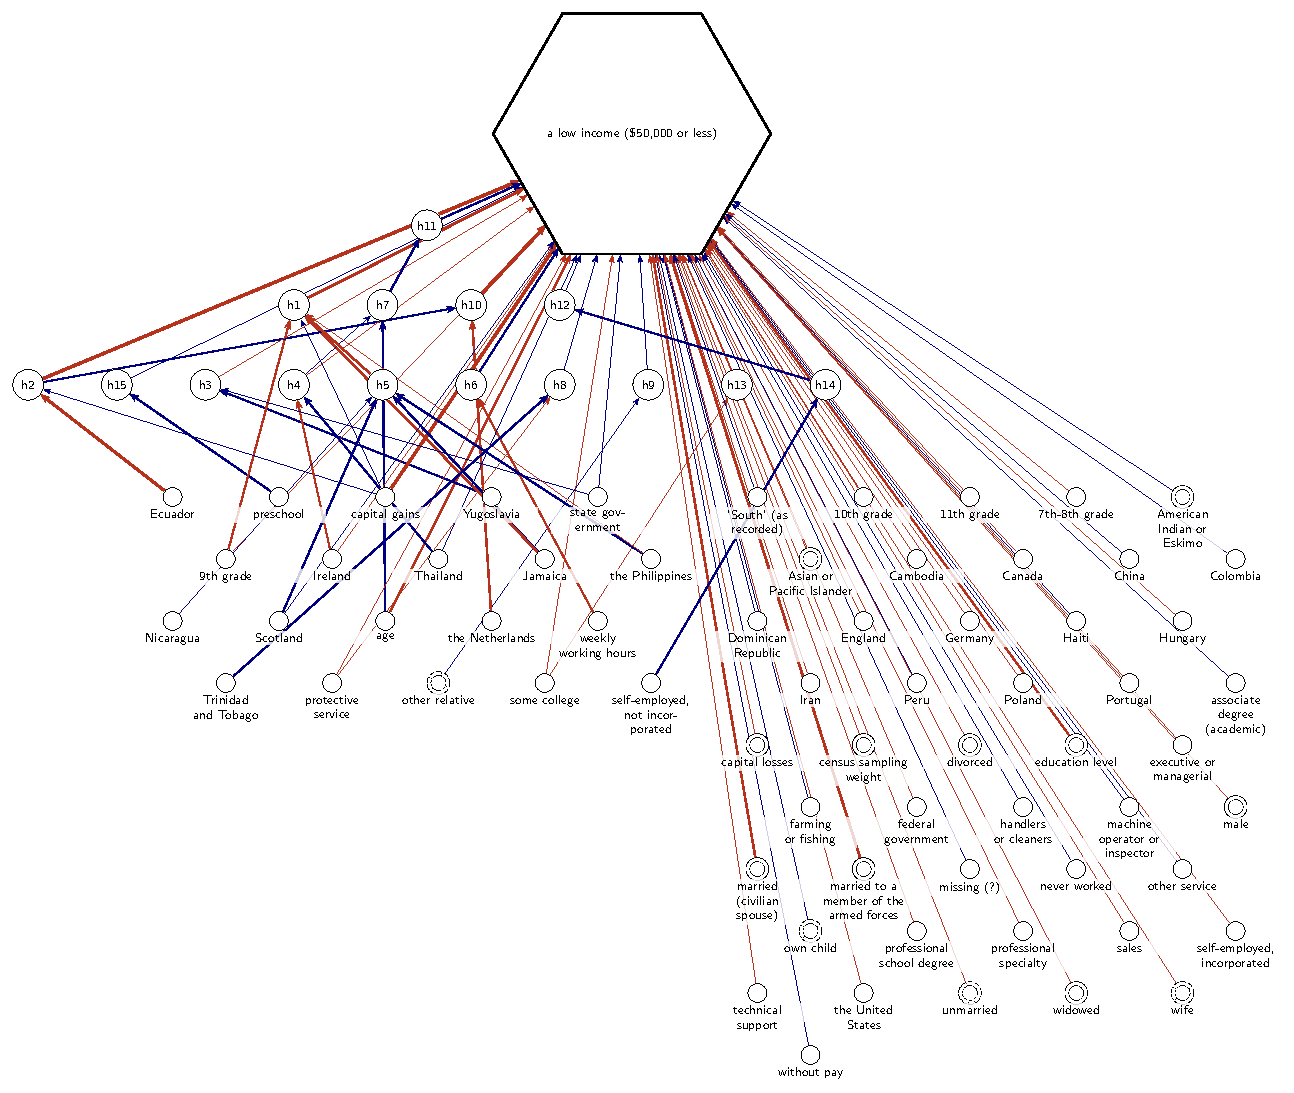
\includegraphics[width=\textheight,height=0.78\textwidth,keepaspectratio]{figures/exp2/networks/adult-s5-raw}
  \caption{Adult, seed 5 (adult-s5): the network as trained, before any explanation, in full. Inputs at the bottom (every input column its own node), hidden units by depth, the output at the top; 66 of 107 input columns are connected, with 15 hidden units and 95 enabled connections. Blue: positive weight (raises the score); red: negative weight (lowers it); thicker: larger weight. Orange outline and up arrow: raises the final prediction; teal and down arrow: lowers it; grey and double arrow: depends. Not used (no connection; 41 columns): missing (?), local government, private, doctorate, high-school graduate, master's degree, 12th grade (no diploma), 1st-4th grade, 5th-6th grade, associate degree (vocational), bachelor's degree, married, spouse absent, never married, separated, administrative or clerical, transport or moving, armed forces, craft or repair, private household service, husband, not in a family, Black, other race, White, missing (?), France, Greece, Guatemala, Honduras, Hong Kong, India, Italy, Japan, Laos, Mexico, outlying US territories (Guam, US Virgin Islands), Puerto Rico, Taiwan, Vietnam, Cuba and El Salvador.}
  \label{fig:exp2-net-adult-s5-raw}
\end{sidewaysfigure}

\clearpage
% Generated by thesis/ch7/exp2/networks.py -- do not edit by hand.
\begin{sidewaysfigure}
  \centering
  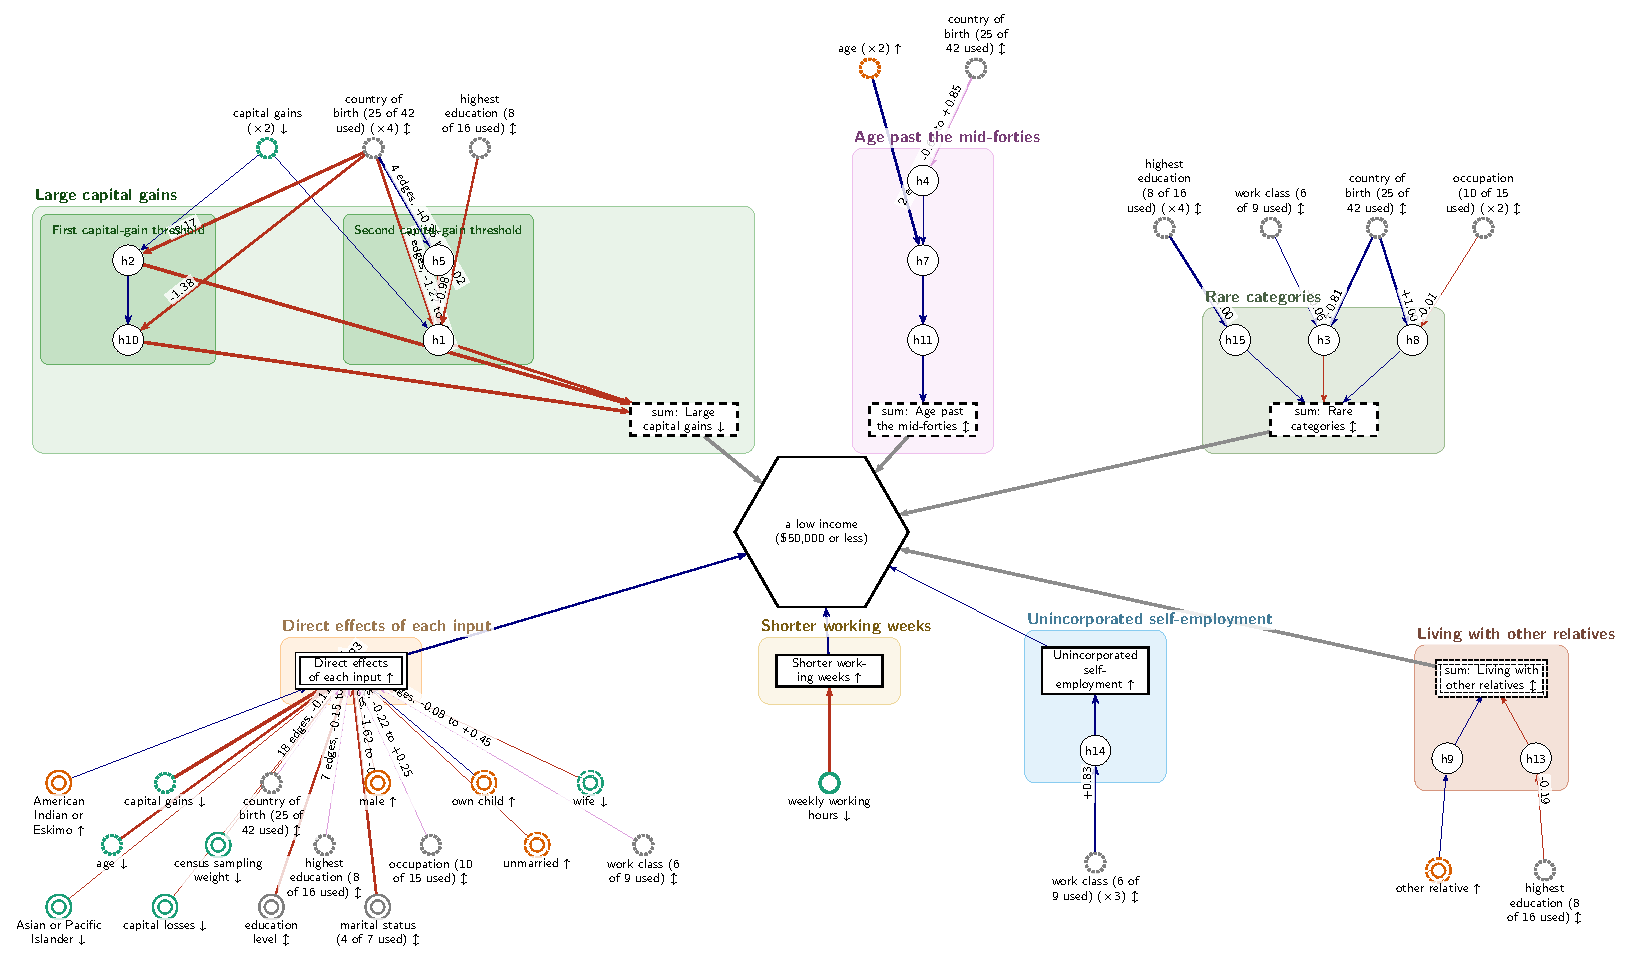
\includegraphics[width=\textheight,height=0.9\textwidth,keepaspectratio]{figures/exp2/networks/adult-s5-explained}
  \caption{Adult, seed 5: the explained network, every unit nested by part.}
  \label{fig:exp2-net-adult-s5-explained}
\end{sidewaysfigure}

\clearpage
% Generated by thesis/ch7/exp2/networks.py -- do not edit by hand.
\begin{sidewaysfigure}
  \centering
  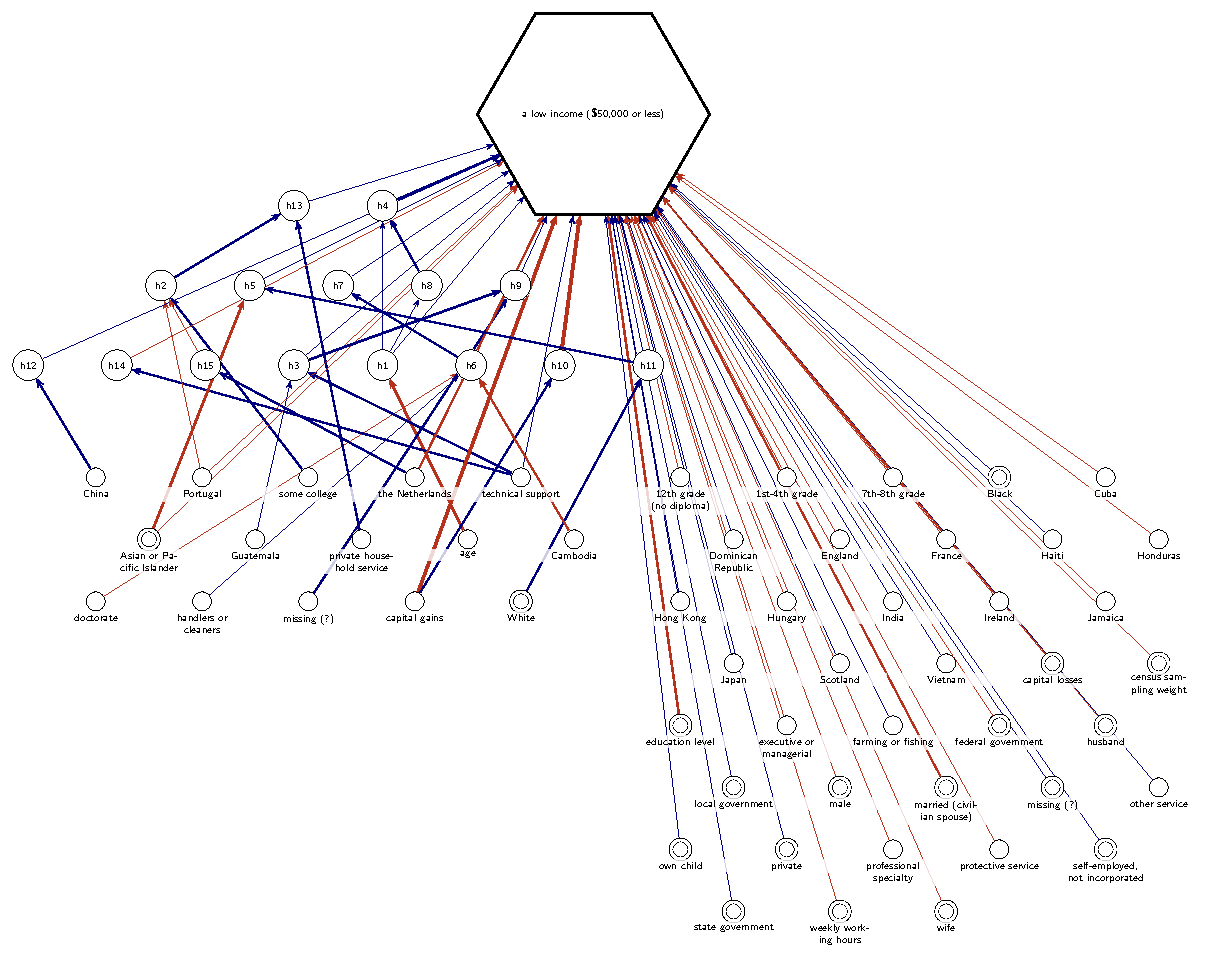
\includegraphics[width=\textheight,height=0.78\textwidth,keepaspectratio]{figures/exp2/networks/adult-s6-raw}
  \caption{Adult, seed 6 (adult-s6): the network as trained, before any explanation, in full. Inputs at the bottom (every input column its own node), hidden units by depth, the output at the top; 53 of 107 input columns are connected, with 15 hidden units and 77 enabled connections. Blue: positive weight (raises the score); red: negative weight (lowers it); thicker: larger weight. Orange outline and up arrow: raises the final prediction; teal and down arrow: lowers it; grey and double arrow: depends. Not used (no connection; 54 columns): never worked, self-employed, incorporated, without pay, 10th grade, 11th grade, high-school graduate, master's degree, preschool, professional school degree, 5th-6th grade, 9th grade, associate degree (academic), associate degree (vocational), bachelor's degree, divorced, married to a member of the armed forces, married, spouse absent, never married, separated, widowed, missing (?), administrative or clerical, sales, transport or moving, armed forces, craft or repair, machine operator or inspector, not in a family, other relative, unmarried, American Indian or Eskimo, other race, Germany, Greece, Canada, Iran, Italy, Laos, Mexico, Nicaragua, outlying US territories (Guam, US Virgin Islands), Peru, the Philippines, Poland, Puerto Rico, 'South' (as recorded), Taiwan, Thailand, Trinidad and Tobago, the United States, Colombia, Yugoslavia, Ecuador and El Salvador.}
  \label{fig:exp2-net-adult-s6-raw}
\end{sidewaysfigure}

\clearpage
% Generated by thesis/ch7/exp2/networks.py -- do not edit by hand.
\ifdefined\netfigheight\else\newlength{\netfigheight}\setlength{\netfigheight}{0.9\textwidth}\fi
\begin{sidewaysfigure}
  \centering
  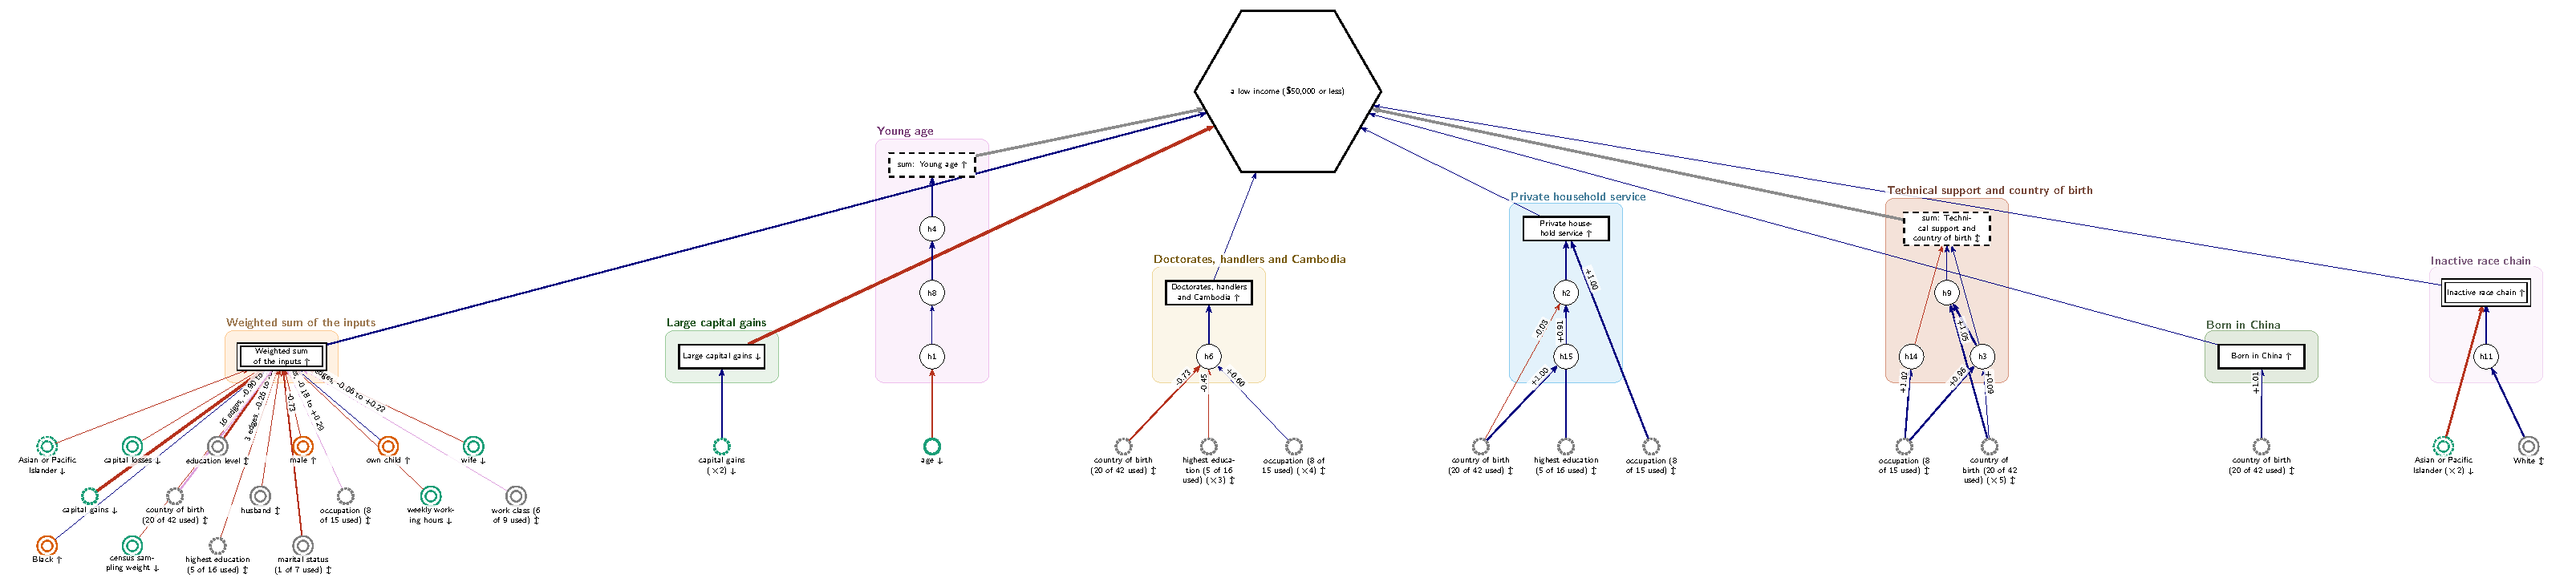
\includegraphics[width=\textheight,height=\netfigheight,keepaspectratio]{figures/exp2/networks/adult-s6-explained}
  \caption{Adult, seed 6: the explained network, every unit nested by part.}
  \label{fig:exp2-net-adult-s6-explained}
\end{sidewaysfigure}

\clearpage
% Generated by thesis/ch7/exp2/networks.py -- do not edit by hand.
\begin{sidewaysfigure}
  \centering
  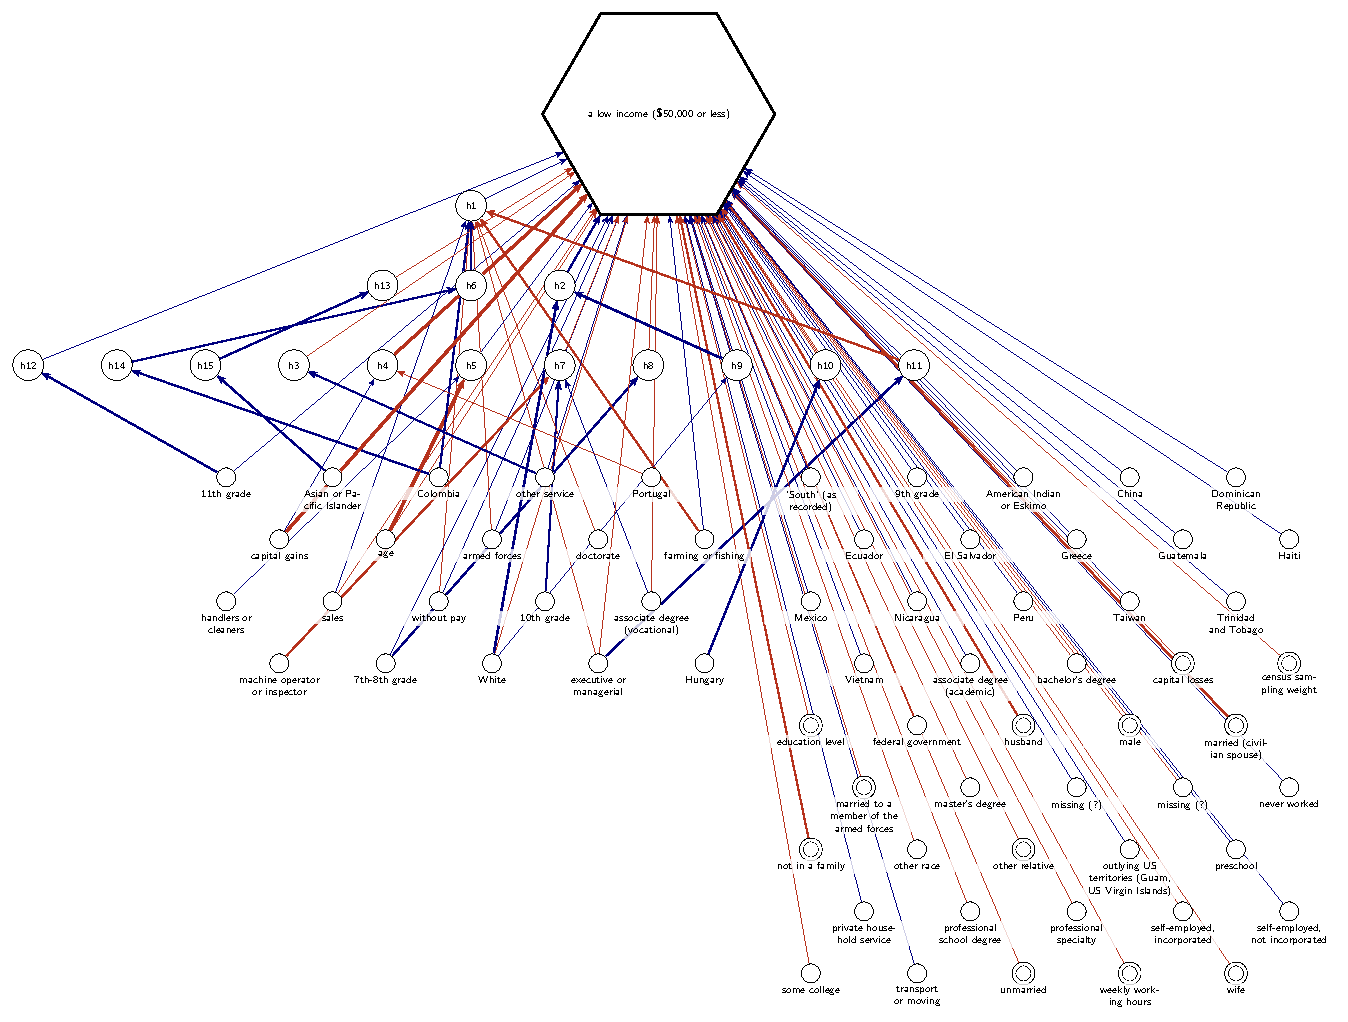
\includegraphics[width=\textheight,height=0.78\textwidth,keepaspectratio]{figures/exp2/networks/adult-s7-raw}
  \caption{Adult, seed 7 (adult-s7): the network as trained, before any explanation, in full. Inputs at the bottom (every input column its own node), hidden units by depth, the output at the top; 65 of 107 input columns are connected, with 15 hidden units and 95 enabled connections. Blue: positive weight (raises the score); red: negative weight (lowers it); thicker: larger weight. Orange outline and up arrow: raises the final prediction; teal and down arrow: lowers it; grey and double arrow: depends. Not used (no connection; 42 columns): local government, private, state government, high-school graduate, 12th grade (no diploma), 1st-4th grade, 5th-6th grade, divorced, married, spouse absent, never married, separated, widowed, administrative or clerical, protective service, technical support, craft or repair, own child, Black, missing (?), Cambodia, France, Germany, the Netherlands, Honduras, Hong Kong, India, Canada, Iran, Ireland, Italy, Jamaica, Japan, Laos, the Philippines, Poland, Puerto Rico, Scotland, Thailand, the United States, Yugoslavia, Cuba and England.}
  \label{fig:exp2-net-adult-s7-raw}
\end{sidewaysfigure}

\clearpage
% Generated by thesis/ch7/exp2/networks.py -- do not edit by hand.
\begin{sidewaysfigure}
  \centering
  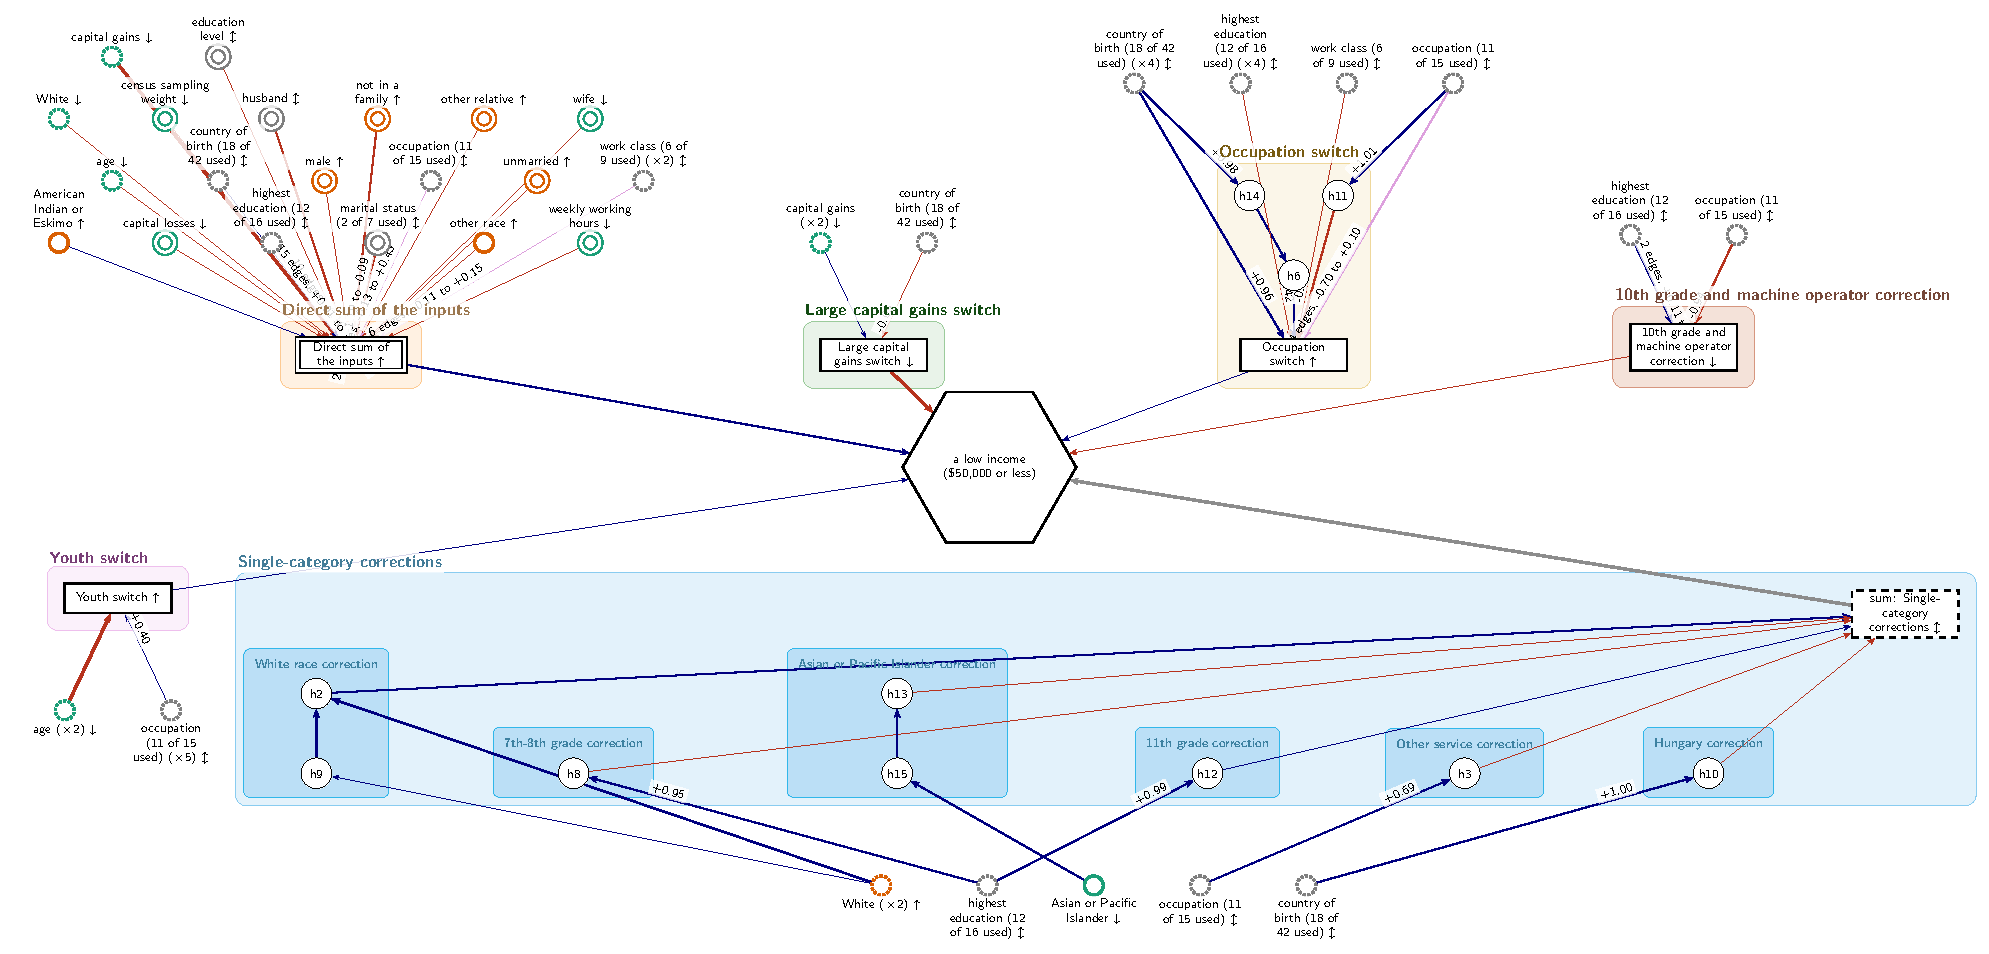
\includegraphics[trim={0.0bp 0 1371.9bp 0},clip,width=\textheight,height=0.78\textwidth,keepaspectratio]{figures/exp2/networks/adult-s7-explained}
  \caption{Adult, seed 7 (adult-s7): every unit and connection of the explained model, nested by part. Shaded clusters are the 13 parts of the agent's explanation (11 leaf and 2 composition annotations, after 12 node splits and 1 identity nodes) and darker boxes the parts inside them; circles are hidden units; each cluster's rectangle is its output, a dashed `sum' an addition the next unit does; the hexagon is the model's output. An input used by several parts is drawn under each of them (dotted outline). Blue: positive weight (raises the score); red: negative weight (lowers it); thicker: larger weight. Orange outline and up arrow: raises the final prediction; teal and down arrow: lowers it; grey and double arrow: depends. Drawn in 3 pieces, left to right, on this and the next 2 pages.}
  \label{fig:exp2-net-adult-s7-explained}
\end{sidewaysfigure}
\clearpage
\begin{sidewaysfigure}
  \centering
  \ContinuedFloat
  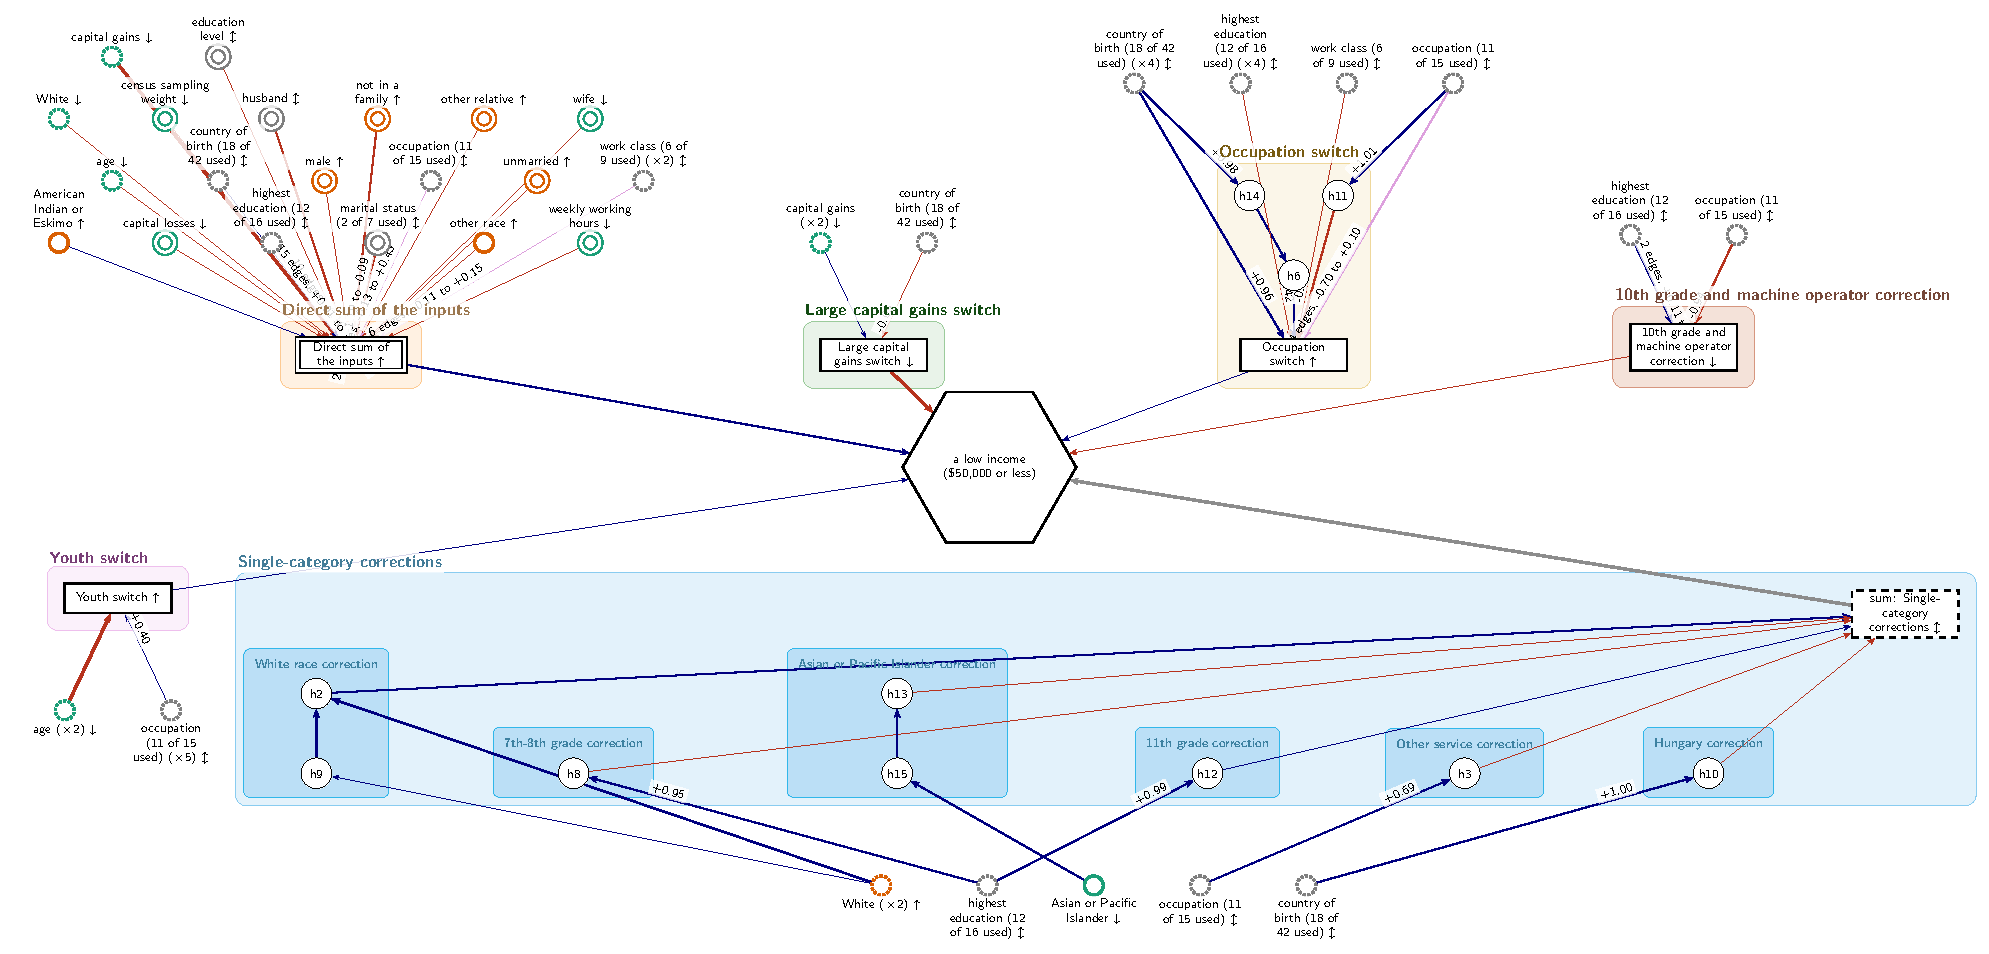
\includegraphics[trim={679.9bp 0 679.9bp 0},clip,width=\textheight,height=0.78\textwidth,keepaspectratio]{figures/exp2/networks/adult-s7-explained}
  \caption[]{(continued, piece 2 of 3).}
\end{sidewaysfigure}
\clearpage
\begin{sidewaysfigure}
  \centering
  \ContinuedFloat
  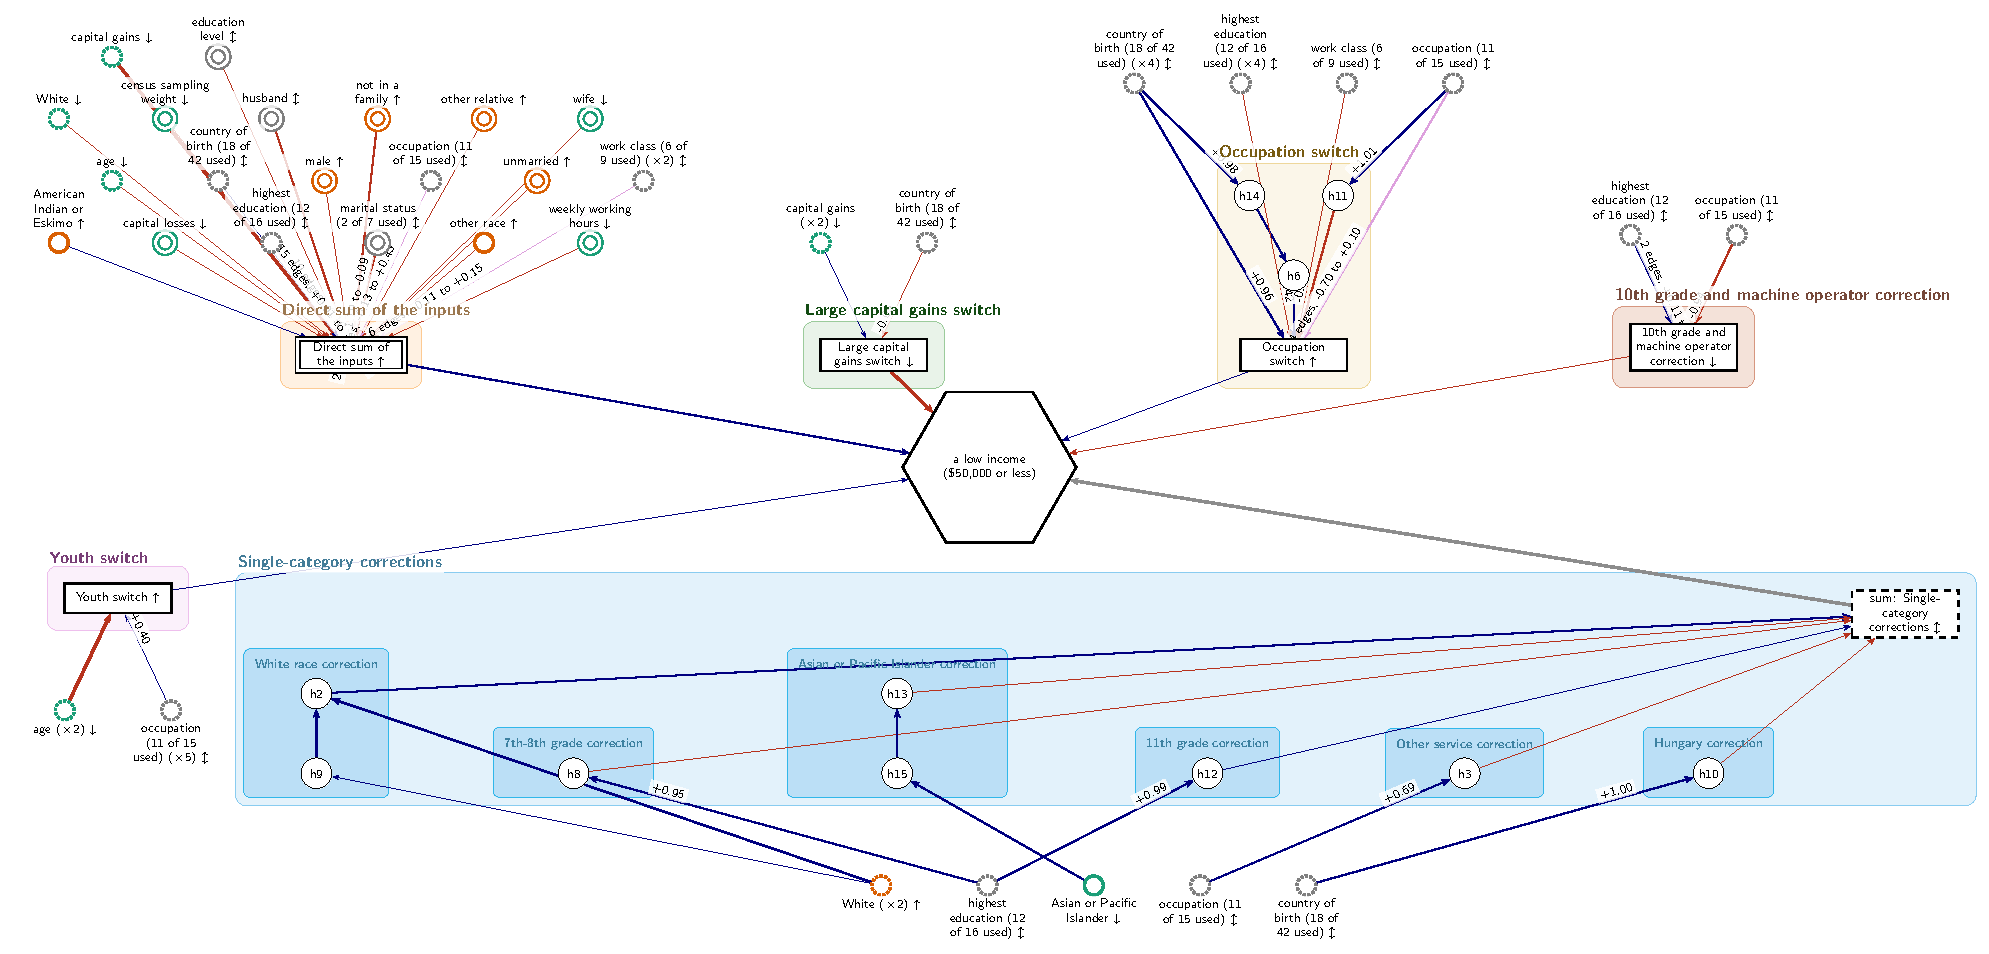
\includegraphics[trim={1371.9bp 0 0.0bp 0},clip,width=\textheight,height=0.78\textwidth,keepaspectratio]{figures/exp2/networks/adult-s7-explained}
  \caption[]{(continued, piece 3 of 3).}
\end{sidewaysfigure}

\clearpage
% Generated by thesis/ch7/exp2/networks.py -- do not edit by hand.
\begin{sidewaysfigure}
  \centering
  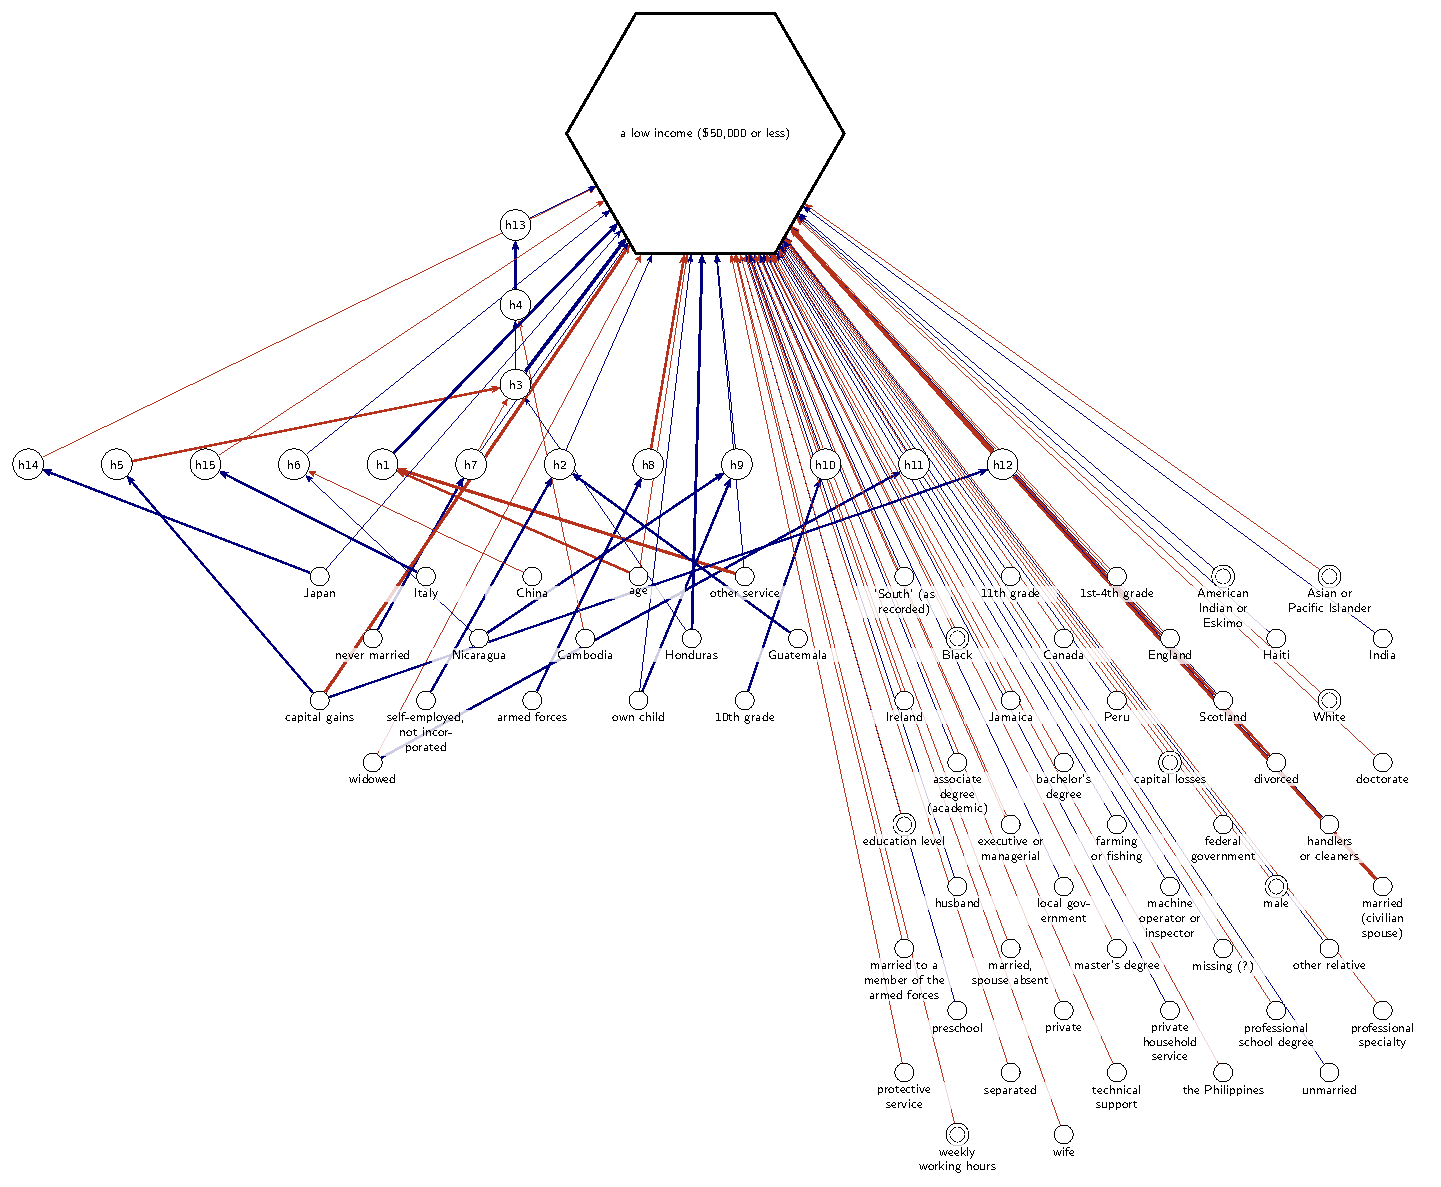
\includegraphics[width=\textheight,height=0.9\textwidth,keepaspectratio]{figures/exp2/networks/adult-s8-raw}
  \caption{Adult, seed 8: the network as trained, before any explanation.}
  \label{fig:exp2-net-adult-s8-raw}
\end{sidewaysfigure}

\clearpage
% Generated by thesis/ch7/exp2/networks.py -- do not edit by hand.
\begin{sidewaysfigure}
  \centering
  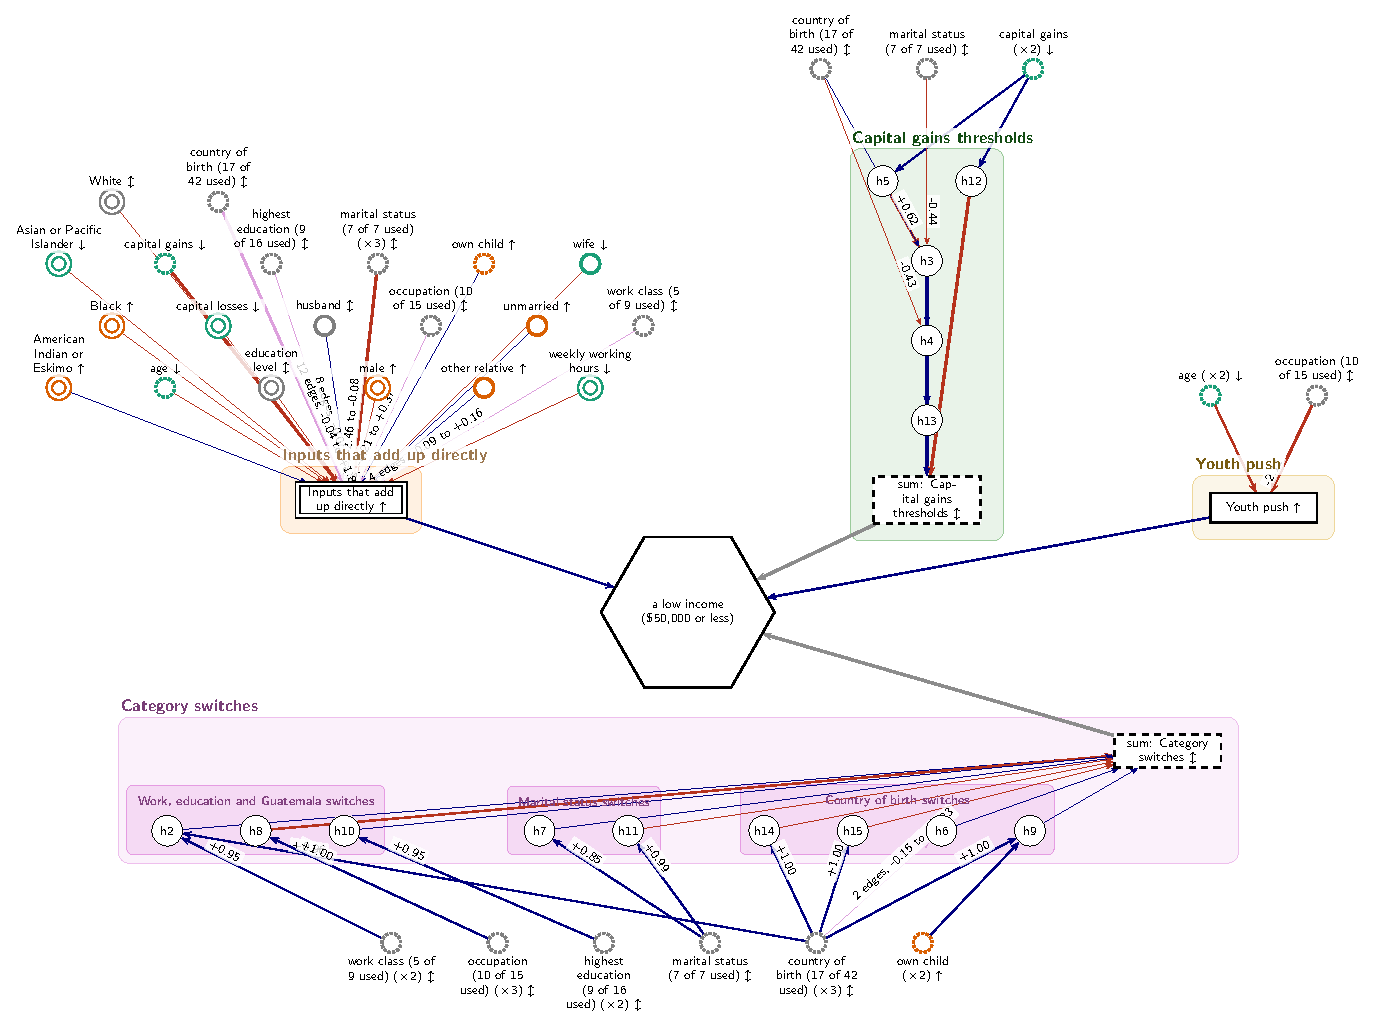
\includegraphics[width=\textheight,height=0.78\textwidth,keepaspectratio]{figures/exp2/networks/adult-s8-explained}
  \caption{Adult, seed 8 (adult-s8): every unit and connection of the explained model, nested by part. Shaded clusters are the 8 parts of the agent's explanation (6 leaf and 2 composition annotations, after 8 node splits and 1 identity nodes) and darker boxes the parts inside them; circles are hidden units; each cluster's rectangle is its output, a dashed `sum' an addition the next unit does; the hexagon is the model's output. An input used by several parts is drawn under each of them (dotted outline). Blue: positive weight (raises the score); red: negative weight (lowers it); thicker: larger weight. Orange outline and up arrow: raises the final prediction; teal and down arrow: lowers it; grey and double arrow: depends.}
  \label{fig:exp2-net-adult-s8-explained}
\end{sidewaysfigure}

\clearpage
% Generated by thesis/ch7/exp2/networks.py -- do not edit by hand.
\begin{sidewaysfigure}
  \centering
  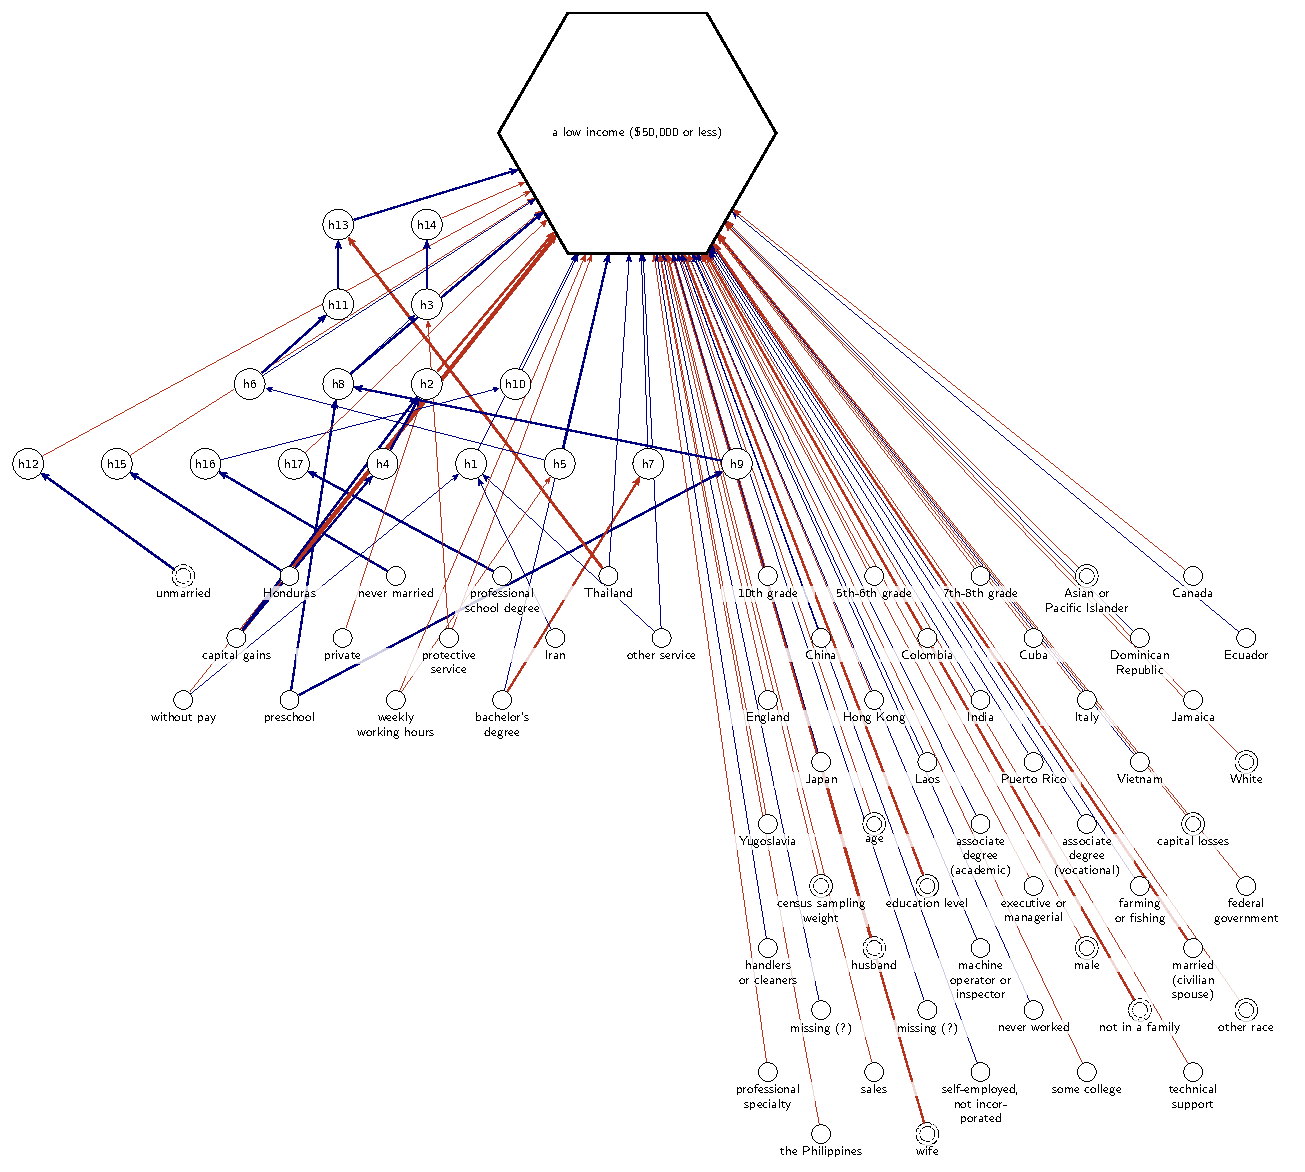
\includegraphics[width=\textheight,height=0.78\textwidth,keepaspectratio]{figures/exp2/networks/adult-s9-raw}
  \caption{Adult, seed 9 (adult-s9): the network as trained, before any explanation, in full. Inputs at the bottom (every input column its own node), hidden units by depth, the output at the top; 61 of 107 input columns are connected, with 17 hidden units and 91 enabled connections. Blue: positive weight (raises the score); red: negative weight (lowers it); thicker: larger weight. Orange outline and up arrow: raises the final prediction; teal and down arrow: lowers it; grey and double arrow: depends. Not used (no connection; 46 columns): local government, self-employed, incorporated, state government, 11th grade, doctorate, high-school graduate, master's degree, 12th grade (no diploma), 1st-4th grade, 9th grade, divorced, married to a member of the armed forces, married, spouse absent, separated, widowed, missing (?), administrative or clerical, transport or moving, armed forces, craft or repair, private household service, other relative, own child, American Indian or Eskimo, Black, Cambodia, France, Germany, Greece, Guatemala, Haiti, the Netherlands, Hungary, Ireland, Mexico, Nicaragua, outlying US territories (Guam, US Virgin Islands), Peru, Poland, Portugal, Scotland, 'South' (as recorded), Taiwan, Trinidad and Tobago, the United States and El Salvador.}
  \label{fig:exp2-net-adult-s9-raw}
\end{sidewaysfigure}

\clearpage
% Generated by thesis/ch7/exp2/networks.py -- do not edit by hand.
\ifdefined\netfigheight\else\newlength{\netfigheight}\setlength{\netfigheight}{0.9\textwidth}\fi
\begin{sidewaysfigure}
  \centering
  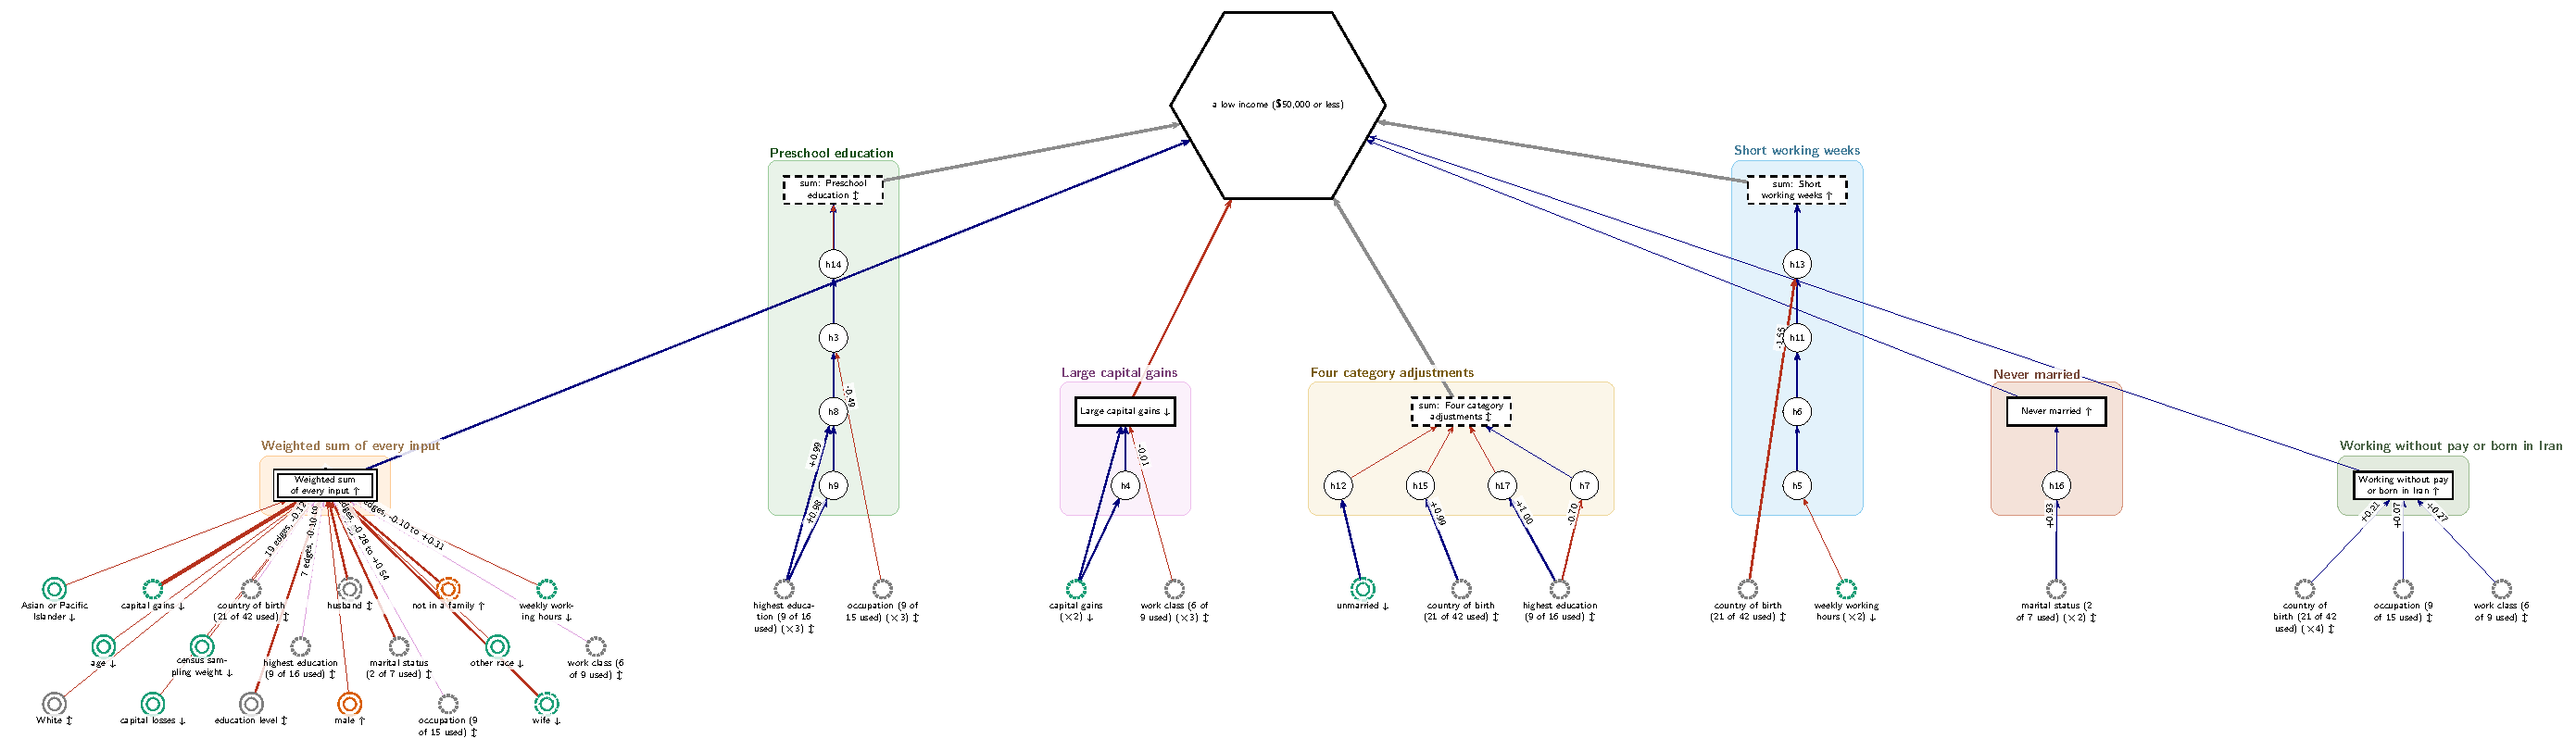
\includegraphics[width=\textheight,height=\netfigheight,keepaspectratio]{figures/exp2/networks/adult-s9-explained}
  \caption{Adult, seed 9: the explained network, every unit nested by part.}
  \label{fig:exp2-net-adult-s9-explained}
\end{sidewaysfigure}

\clearpage
% Churn: the ten networks (the dataset is named in each caption)
% Generated by thesis/ch7/exp2/networks.py -- do not edit by hand.
\begin{sidewaysfigure}
  \centering
  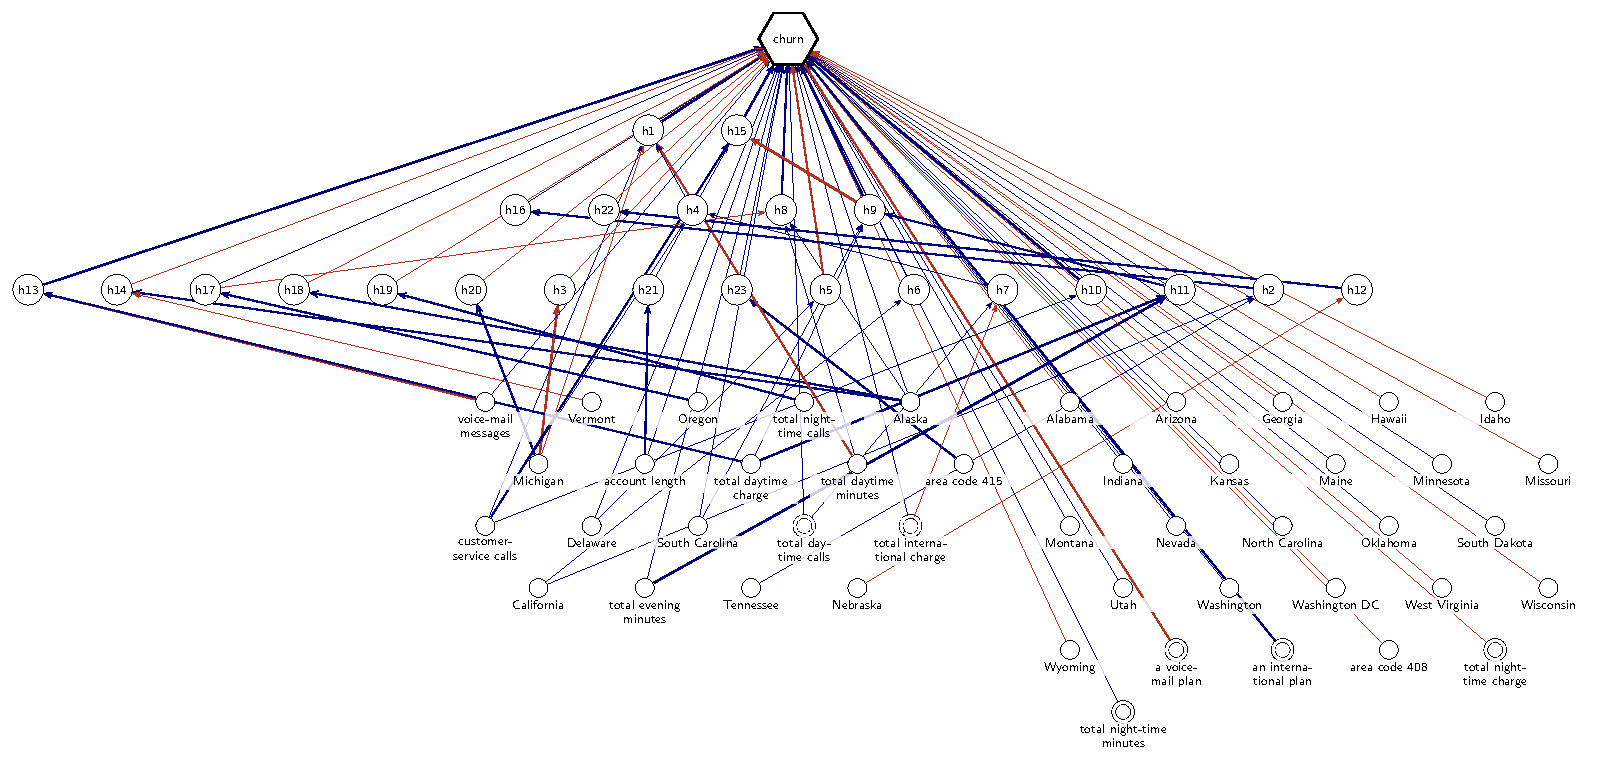
\includegraphics[width=\textheight,height=0.78\textwidth,keepaspectratio]{figures/exp2/networks/churn100-s0-raw}
  \caption{Churn, seed 0 (churn100-s0): the network as trained, before any explanation, in full. Inputs at the bottom (every input column its own node), hidden units by depth, the output at the top; 45 of 71 input columns are connected, with 23 hidden units and 89 enabled connections. Blue: positive weight (raises the score); red: negative weight (lowers it); thicker: larger weight. Orange outline and up arrow: raises the final prediction; teal and down arrow: lowers it; grey and double arrow: depends. Not used (no connection; 26 columns): Iowa, Illinois, Kentucky, Louisiana, Massachusetts, Arkansas, Maryland, Mississippi, North Dakota, New Hampshire, New Jersey, New Mexico, New York, Ohio, Pennsylvania, Rhode Island, Texas, Virginia, Colorado, Connecticut, Florida, area code 510, total evening calls, total evening charge, total international minutes and total international calls.}
  \label{fig:exp2-net-churn100-s0-raw}
\end{sidewaysfigure}

\clearpage
% Generated by thesis/ch7/exp2/networks.py -- do not edit by hand.
\begin{sidewaysfigure}
  \centering
  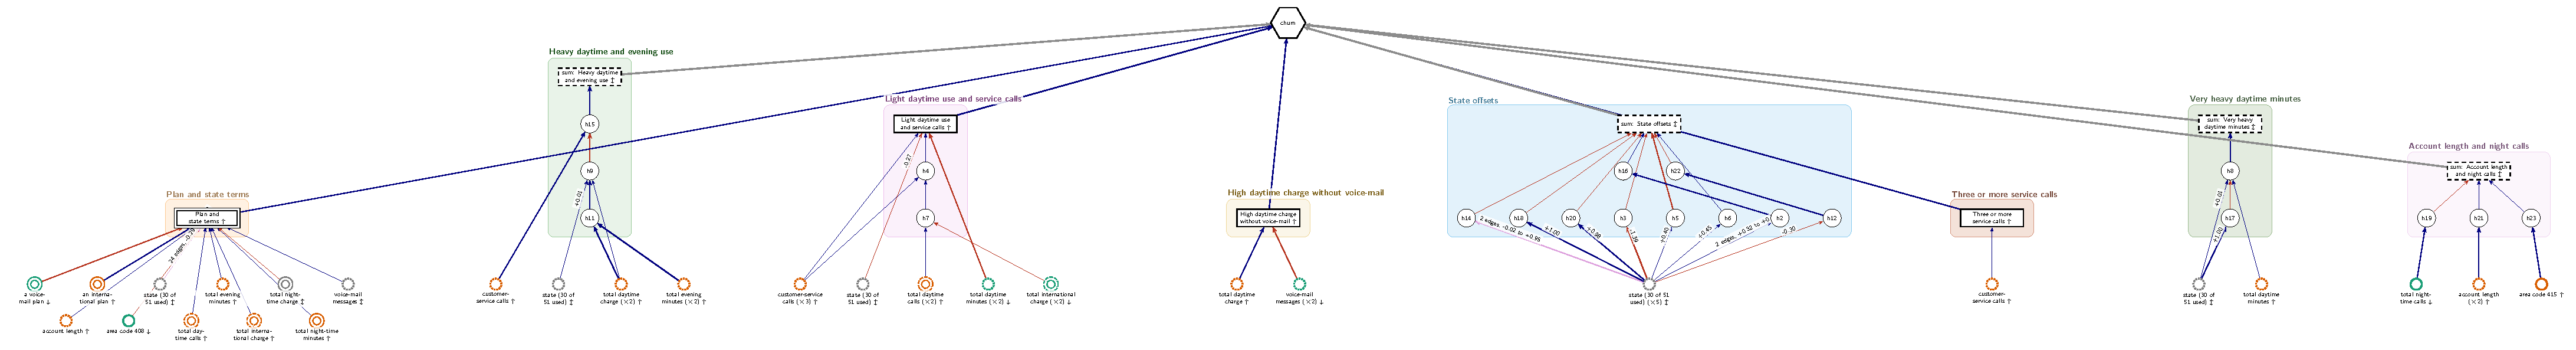
\includegraphics[trim={0.0bp 0 1385.9bp 0},clip,width=\textheight,height=0.78\textwidth,keepaspectratio]{figures/exp2/networks/churn100-s0-explained}
  \caption{Churn, seed 0 (churn100-s0): every unit and connection of the explained model, nested by part. Shaded clusters are the 9 parts of the agent's explanation (8 leaf and 1 composition annotations, after 12 node splits and 1 identity nodes) and darker boxes the parts inside them; circles are hidden units; each cluster's rectangle is its output, a dashed `sum' an addition the next unit does; the hexagon is the model's output. An input used by several parts is drawn under each of them (dotted outline). Blue: positive weight (raises the score); red: negative weight (lowers it); thicker: larger weight. Orange outline and up arrow: raises the final prediction; teal and down arrow: lowers it; grey and double arrow: depends. Drawn in 3 pieces, left to right, on this and the next 2 pages.}
  \label{fig:exp2-net-churn100-s0-explained}
\end{sidewaysfigure}
\clearpage
\begin{sidewaysfigure}
  \centering
  \ContinuedFloat
  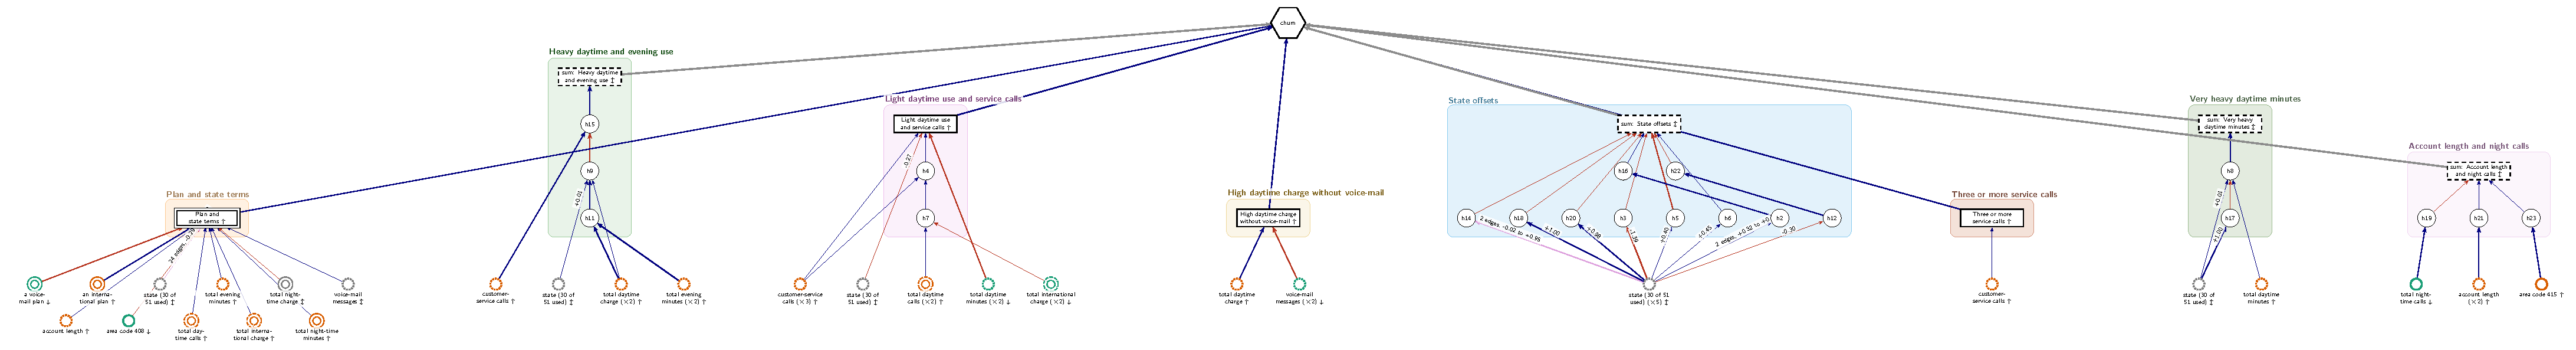
\includegraphics[trim={686.9bp 0 687.0bp 0},clip,width=\textheight,height=0.78\textwidth,keepaspectratio]{figures/exp2/networks/churn100-s0-explained}
  \caption[]{(continued, piece 2 of 3).}
\end{sidewaysfigure}
\clearpage
\begin{sidewaysfigure}
  \centering
  \ContinuedFloat
  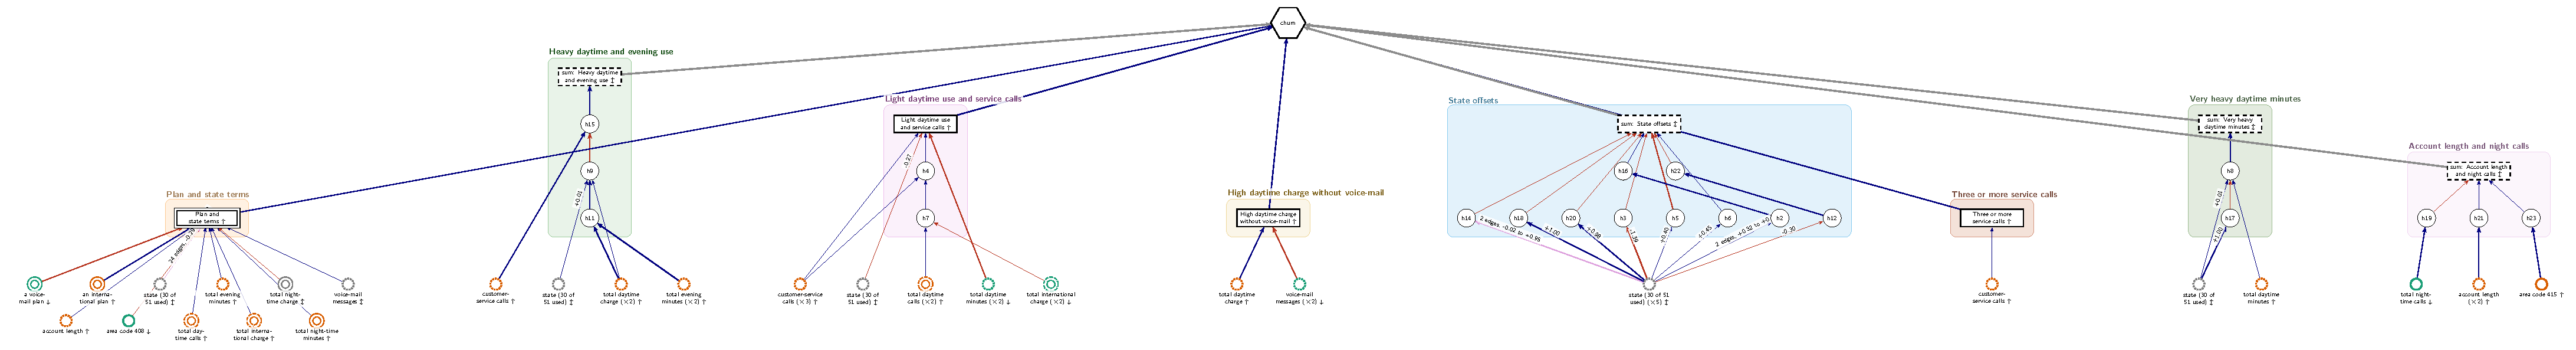
\includegraphics[trim={1385.9bp 0 0.0bp 0},clip,width=\textheight,height=0.78\textwidth,keepaspectratio]{figures/exp2/networks/churn100-s0-explained}
  \caption[]{(continued, piece 3 of 3).}
\end{sidewaysfigure}

\clearpage
% Generated by thesis/ch7/exp2/networks.py -- do not edit by hand.
\begin{sidewaysfigure}
  \centering
  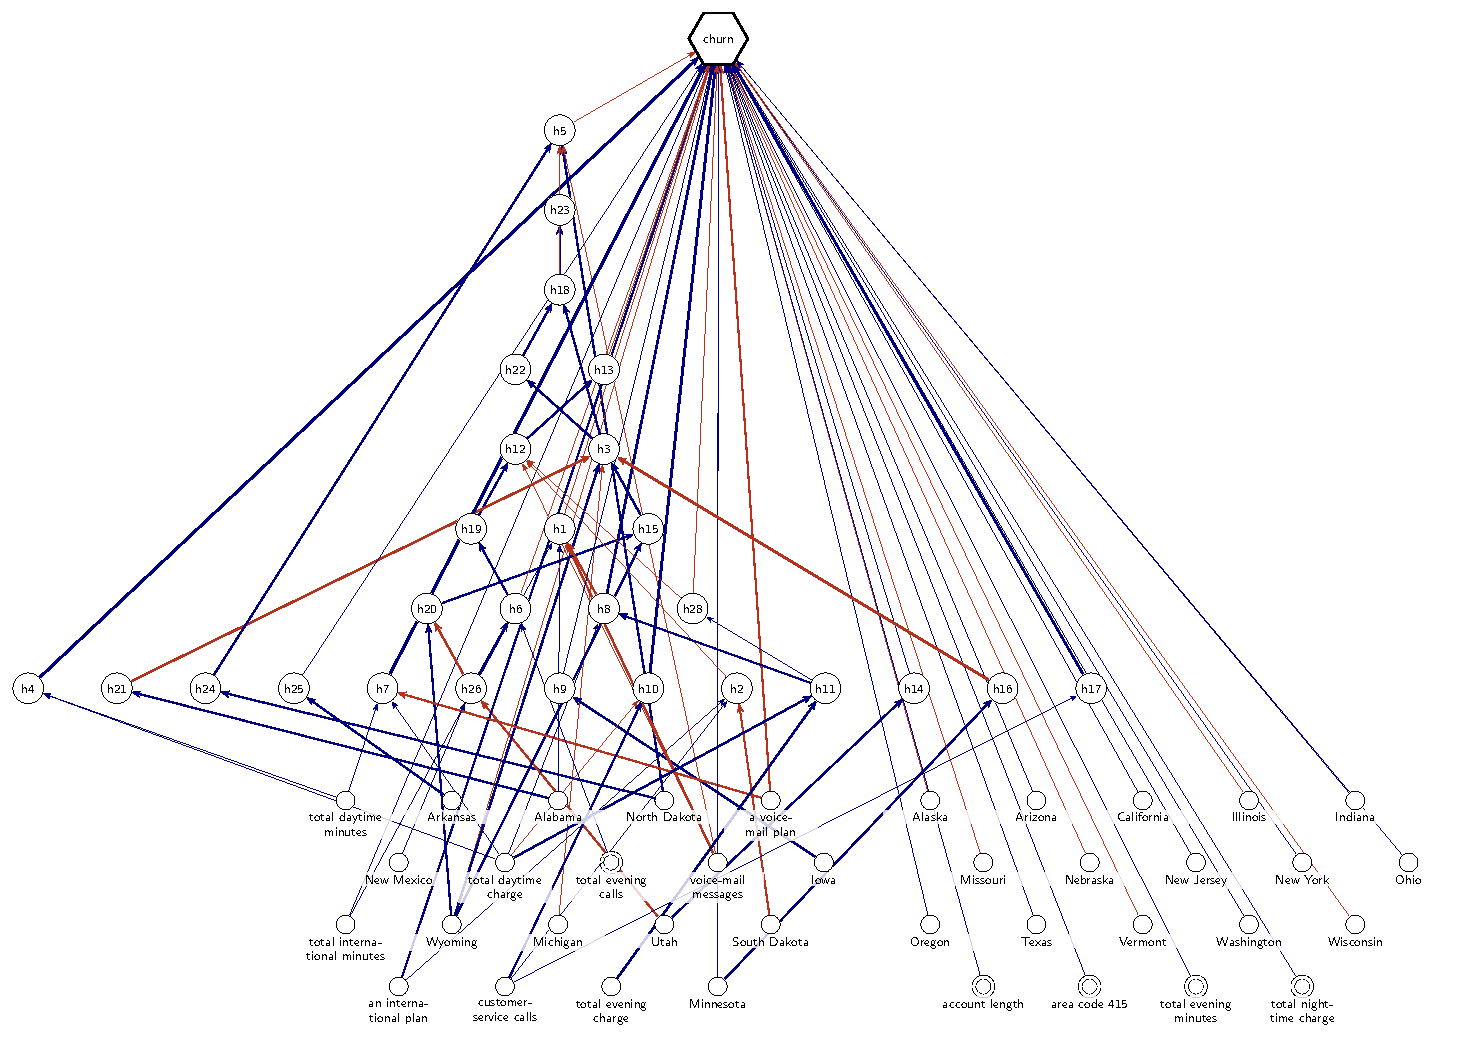
\includegraphics[width=\textheight,height=0.78\textwidth,keepaspectratio]{figures/exp2/networks/churn100-s1-raw}
  \caption{Churn, seed 1 (churn100-s1): the network as trained, before any explanation, in full. Inputs at the bottom (every input column its own node), hidden units by depth, the output at the top; 38 of 71 input columns are connected, with 27 hidden units and 92 enabled connections. Blue: positive weight (raises the score); red: negative weight (lowers it); thicker: larger weight. Orange outline and up arrow: raises the final prediction; teal and down arrow: lowers it; grey and double arrow: depends. Not used (no connection; 33 columns): Georgia, Hawaii, Idaho, Kansas, Kentucky, Louisiana, Massachusetts, Maryland, Maine, Mississippi, Montana, North Carolina, New Hampshire, Nevada, Oklahoma, Pennsylvania, Rhode Island, South Carolina, Tennessee, Virginia, West Virginia, Colorado, Connecticut, Washington DC, Delaware, Florida, area code 408, area code 510, total daytime calls, total night-time minutes, total night-time calls, total international calls and total international charge.}
  \label{fig:exp2-net-churn100-s1-raw}
\end{sidewaysfigure}

\clearpage
% Generated by thesis/ch7/exp2/networks.py -- do not edit by hand.
\ifdefined\netfigheight\else\newlength{\netfigheight}\setlength{\netfigheight}{0.9\textwidth}\fi
\begin{sidewaysfigure}
  \centering
  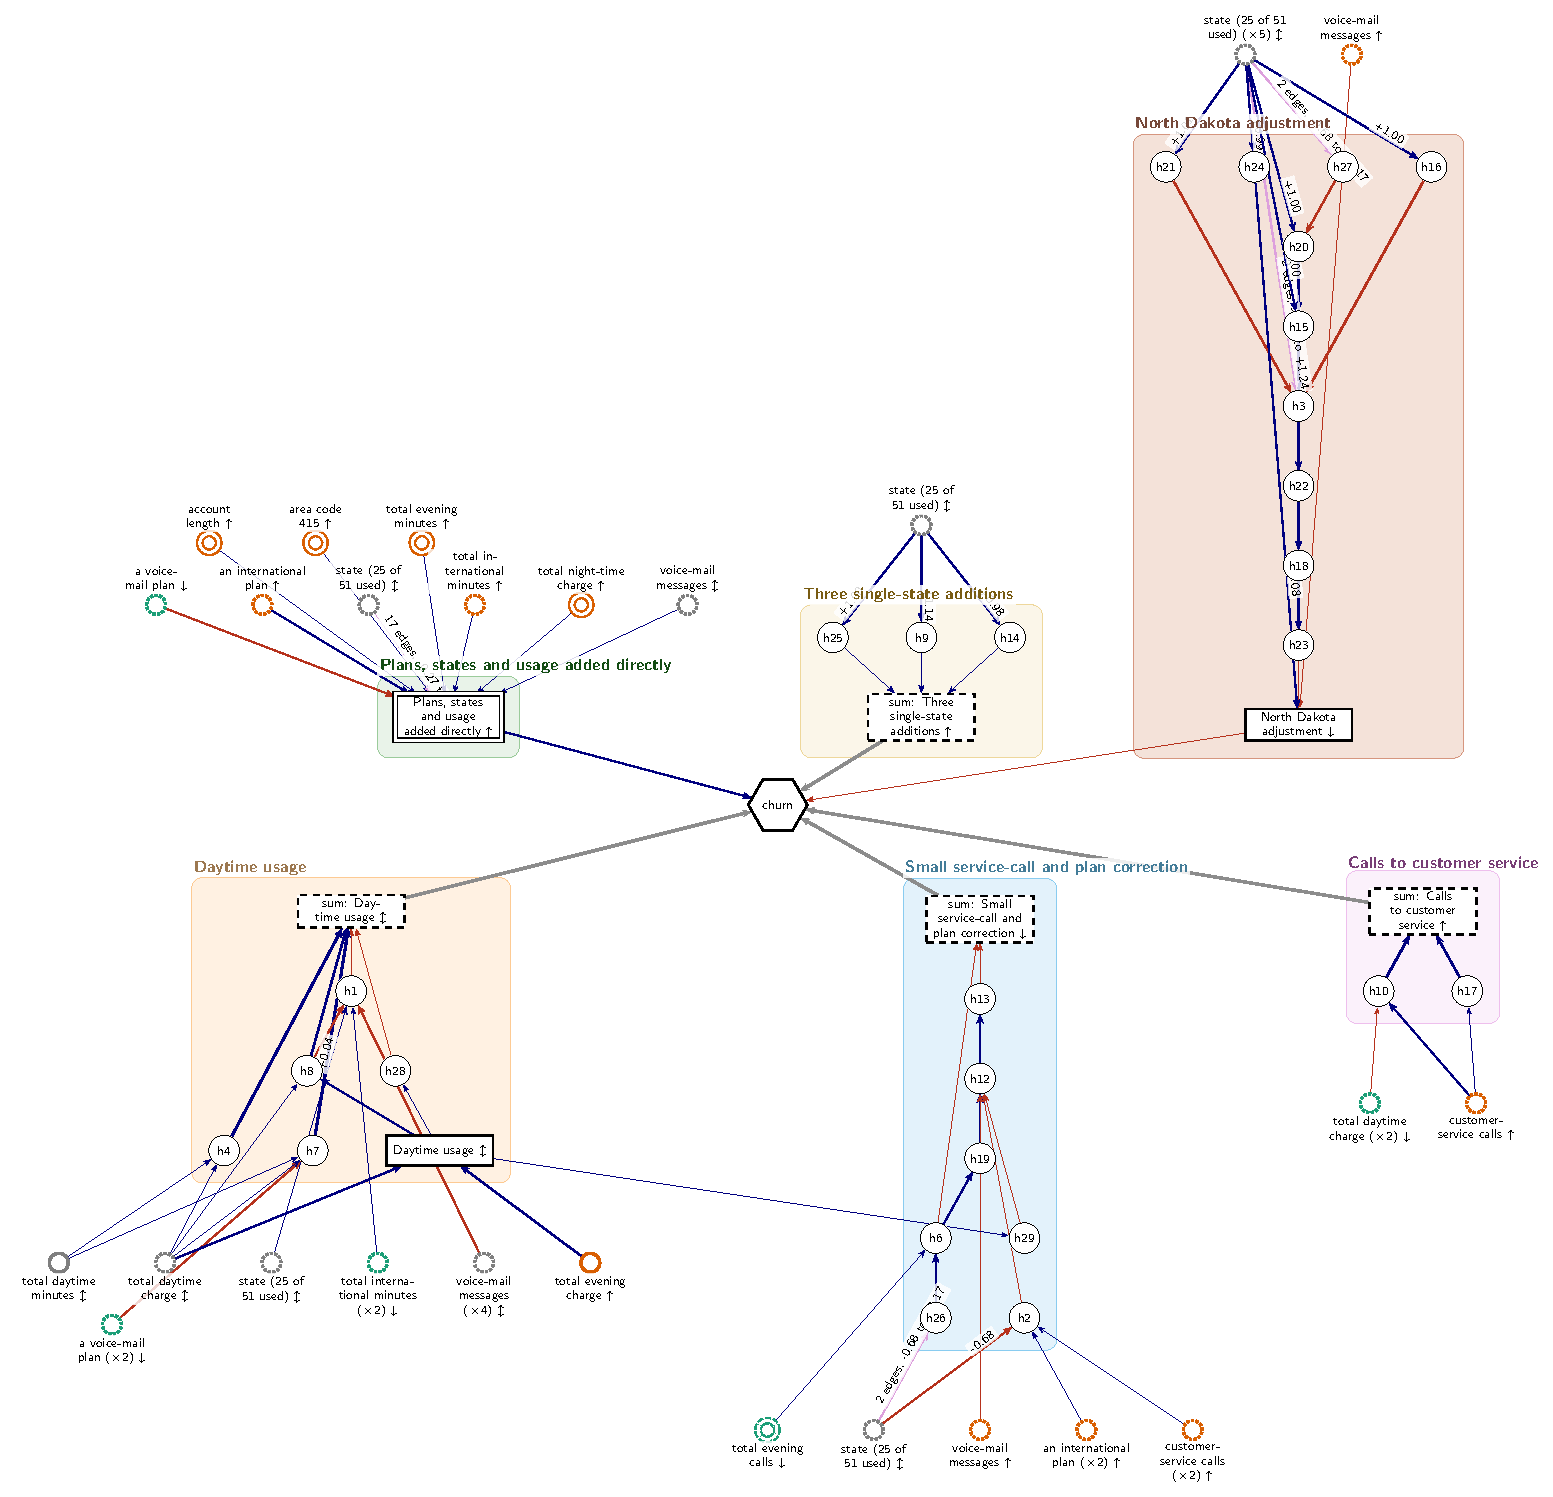
\includegraphics[width=\textheight,height=\netfigheight,keepaspectratio]{figures/exp2/networks/churn100-s1-explained}
  \caption{Churn, seed 1: the explained network, every unit nested by part.}
  \label{fig:exp2-net-churn100-s1-explained}
\end{sidewaysfigure}

\clearpage
% Generated by thesis/ch7/exp2/networks.py -- do not edit by hand.
\begin{sidewaysfigure}
  \centering
  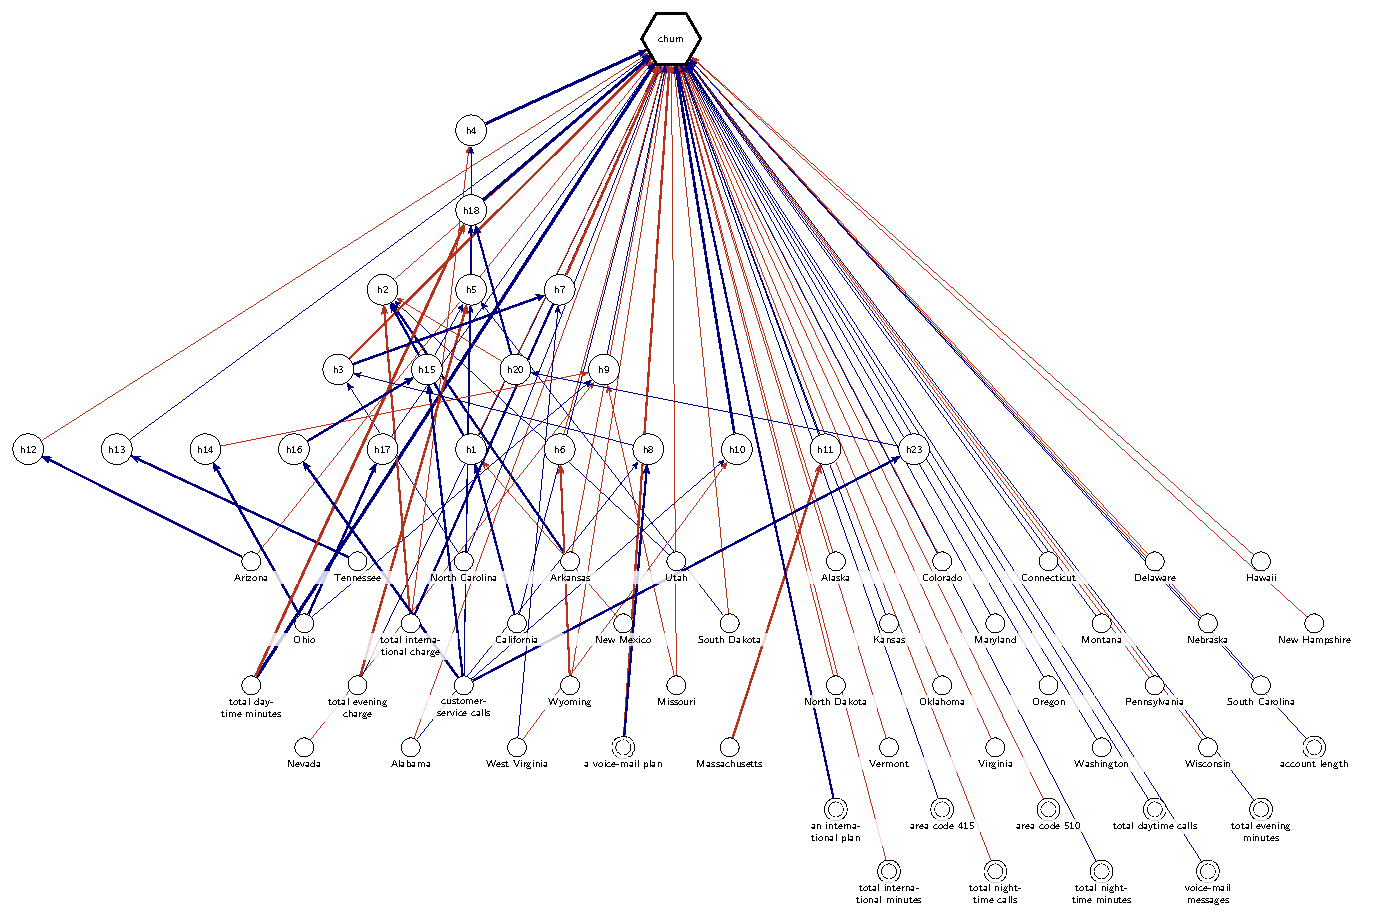
\includegraphics[width=\textheight,height=0.78\textwidth,keepaspectratio]{figures/exp2/networks/churn100-s2-raw}
  \caption{Churn, seed 2 (churn100-s2): the network as trained, before any explanation, in full. Inputs at the bottom (every input column its own node), hidden units by depth, the output at the top; 49 of 71 input columns are connected, with 20 hidden units and 94 enabled connections. Blue: positive weight (raises the score); red: negative weight (lowers it); thicker: larger weight. Orange outline and up arrow: raises the final prediction; teal and down arrow: lowers it; grey and double arrow: depends. Not used (no connection; 22 columns): Georgia, Iowa, Idaho, Illinois, Indiana, Kentucky, Louisiana, Maine, Michigan, Minnesota, Mississippi, New Jersey, New York, Rhode Island, Texas, Washington DC, Florida, area code 408, total daytime charge, total evening calls, total night-time charge and total international calls.}
  \label{fig:exp2-net-churn100-s2-raw}
\end{sidewaysfigure}

\clearpage
% Generated by thesis/ch7/exp2/networks.py -- do not edit by hand.
\ifdefined\netfigheight\else\newlength{\netfigheight}\setlength{\netfigheight}{0.9\textwidth}\fi
\begin{sidewaysfigure}
  \centering
  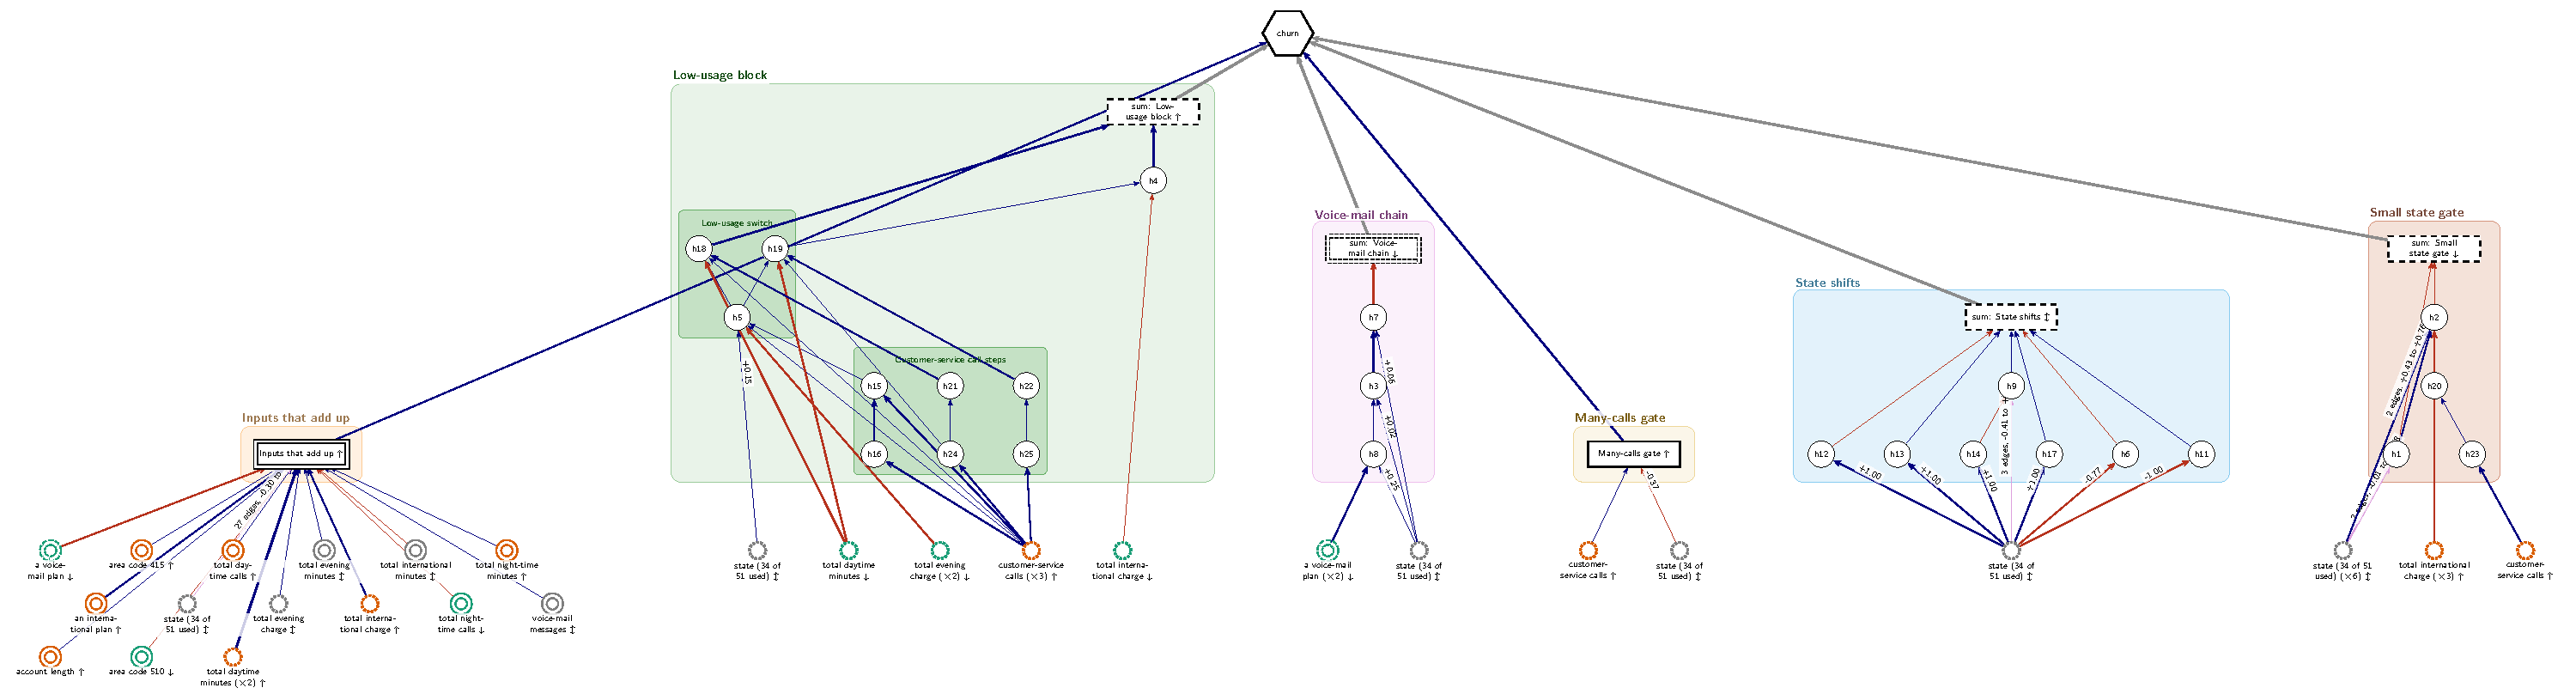
\includegraphics[width=\textheight,height=\netfigheight,keepaspectratio]{figures/exp2/networks/churn100-s2-explained}
  \caption{Churn, seed 2: the explained network, every unit nested by part.}
  \label{fig:exp2-net-churn100-s2-explained}
\end{sidewaysfigure}

\clearpage
% Generated by thesis/ch7/exp2/networks.py -- do not edit by hand.
\begin{sidewaysfigure}
  \centering
  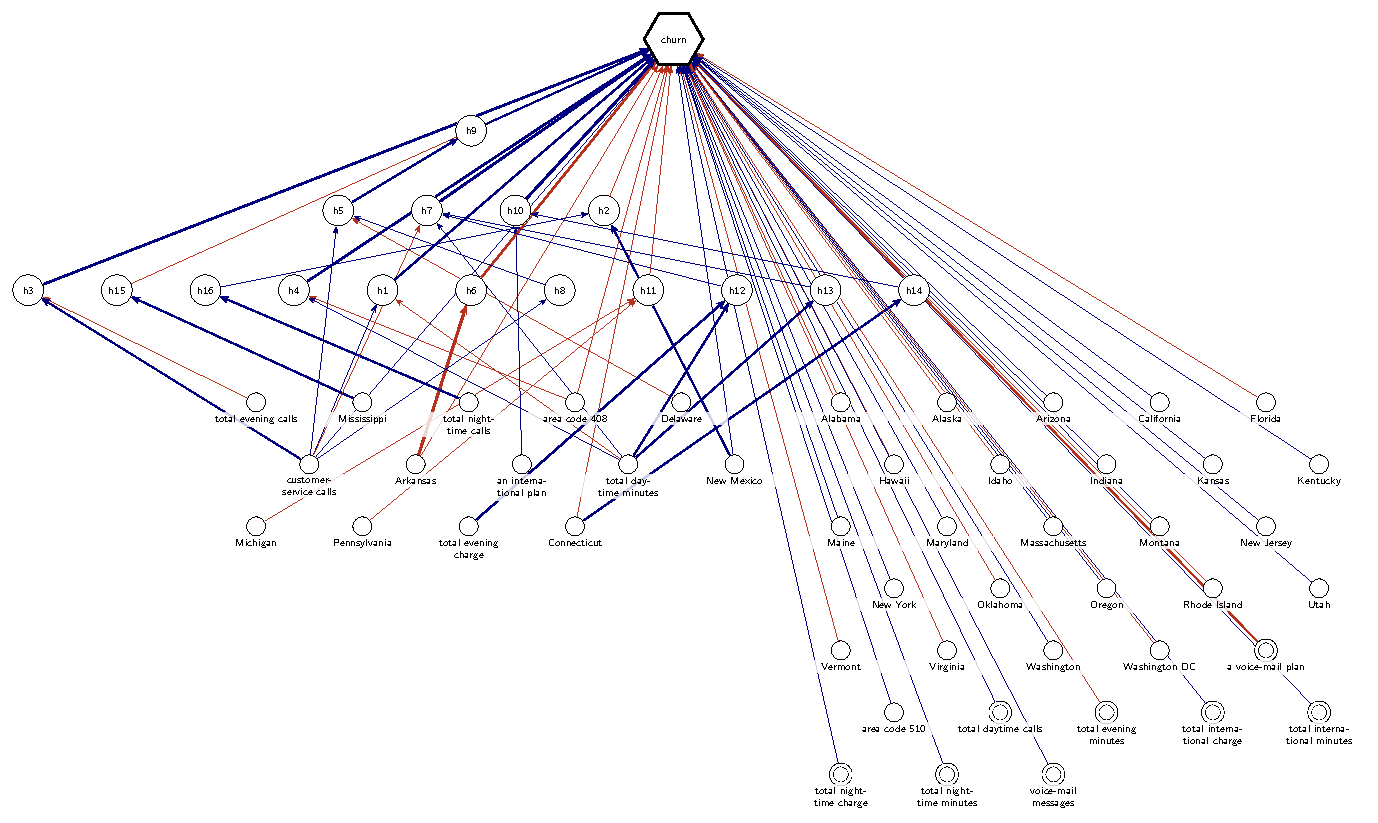
\includegraphics[width=\textheight,height=0.78\textwidth,keepaspectratio]{figures/exp2/networks/churn100-s3-raw}
  \caption{Churn, seed 3 (churn100-s3): the network as trained, before any explanation, in full. Inputs at the bottom (every input column its own node), hidden units by depth, the output at the top; 47 of 71 input columns are connected, with 16 hidden units and 77 enabled connections. Blue: positive weight (raises the score); red: negative weight (lowers it); thicker: larger weight. Orange outline and up arrow: raises the final prediction; teal and down arrow: lowers it; grey and double arrow: depends. Not used (no connection; 24 columns): Georgia, Iowa, Illinois, Louisiana, Minnesota, Missouri, North Carolina, North Dakota, Nebraska, New Hampshire, Nevada, Ohio, South Carolina, South Dakota, Tennessee, Texas, Wisconsin, West Virginia, Colorado, Wyoming, account length, area code 415, total daytime charge and total international calls.}
  \label{fig:exp2-net-churn100-s3-raw}
\end{sidewaysfigure}

\clearpage
% Generated by thesis/ch7/exp2/networks.py -- do not edit by hand.
\begin{sidewaysfigure}
  \centering
  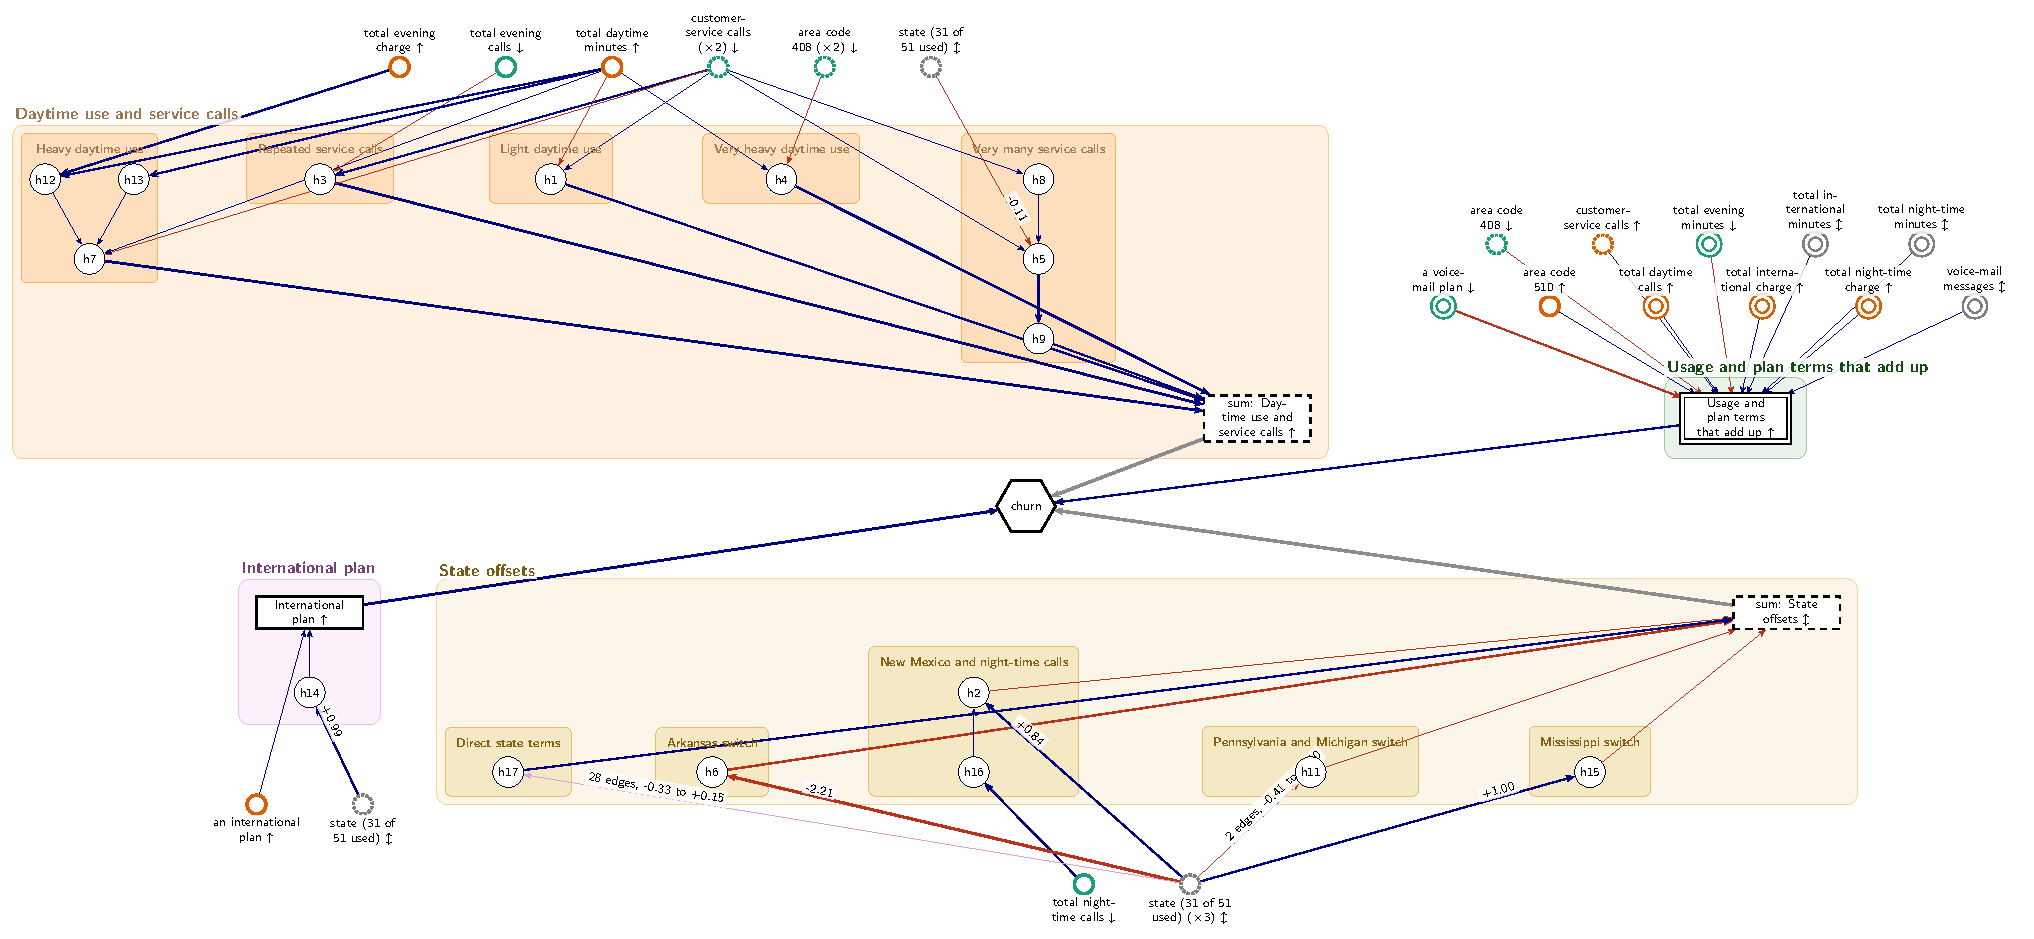
\includegraphics[width=\textheight,height=0.78\textwidth,keepaspectratio]{figures/exp2/networks/churn100-s3-explained}
  \caption{Churn, seed 3 (churn100-s3): every unit and connection of the explained model, nested by part. Shaded clusters are the 15 parts of the agent's explanation (12 leaf and 3 composition annotations, after 7 node splits and 2 identity nodes) and darker boxes the parts inside them; circles are hidden units; each cluster's rectangle is its output, a dashed `sum' an addition the next unit does; the hexagon is the model's output. An input used by several parts is drawn under each of them (dotted outline). Blue: positive weight (raises the score); red: negative weight (lowers it); thicker: larger weight. Orange outline and up arrow: raises the final prediction; teal and down arrow: lowers it; grey and double arrow: depends.}
  \label{fig:exp2-net-churn100-s3-explained}
\end{sidewaysfigure}

\clearpage
% Generated by thesis/ch7/exp2/networks.py -- do not edit by hand.
\begin{sidewaysfigure}
  \centering
  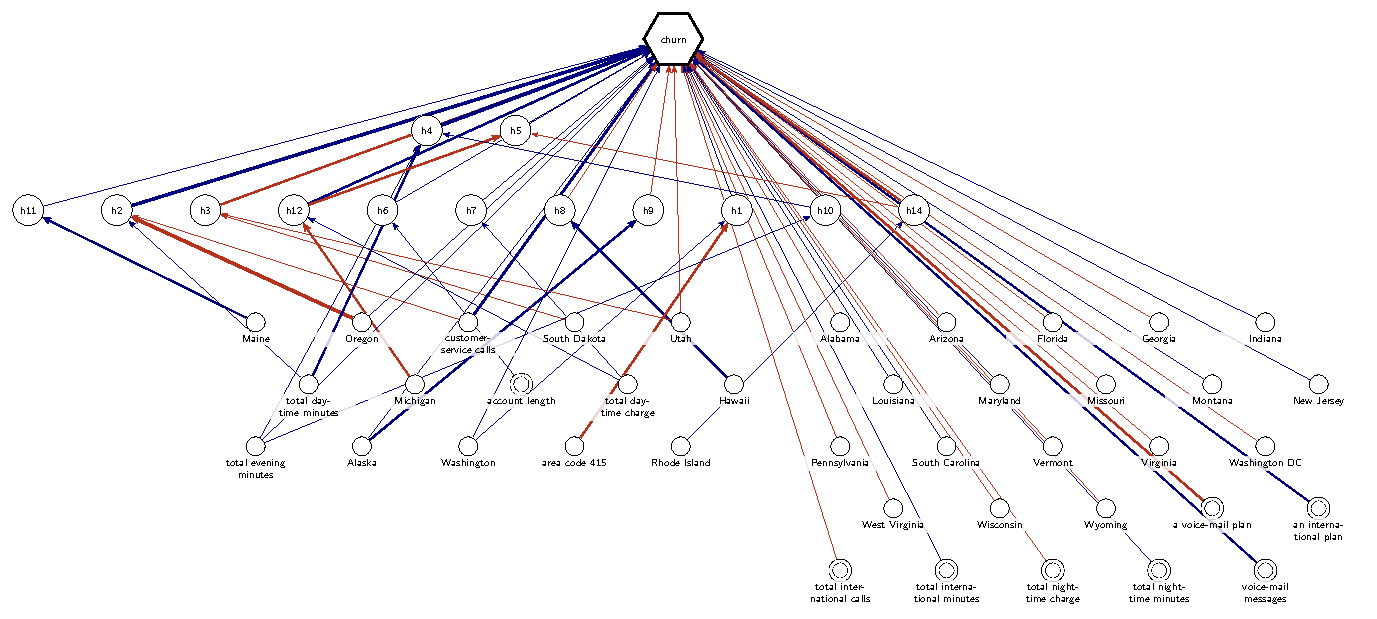
\includegraphics[width=\textheight,height=0.78\textwidth,keepaspectratio]{figures/exp2/networks/churn100-s4-raw}
  \caption{Churn, seed 4 (churn100-s4): the network as trained, before any explanation, in full. Inputs at the bottom (every input column its own node), hidden units by depth, the output at the top; 40 of 71 input columns are connected, with 13 hidden units and 64 enabled connections. Blue: positive weight (raises the score); red: negative weight (lowers it); thicker: larger weight. Orange outline and up arrow: raises the final prediction; teal and down arrow: lowers it; grey and double arrow: depends. Not used (no connection; 31 columns): Iowa, Idaho, Illinois, Kansas, Kentucky, Massachusetts, Arkansas, Minnesota, Mississippi, North Carolina, North Dakota, Nebraska, New Hampshire, New Mexico, Nevada, New York, Ohio, Oklahoma, California, Tennessee, Texas, Colorado, Connecticut, Delaware, area code 408, area code 510, total daytime calls, total evening calls, total evening charge, total night-time calls and total international charge.}
  \label{fig:exp2-net-churn100-s4-raw}
\end{sidewaysfigure}

\clearpage
% Generated by thesis/ch7/exp2/networks.py -- do not edit by hand.
\begin{sidewaysfigure}
  \centering
  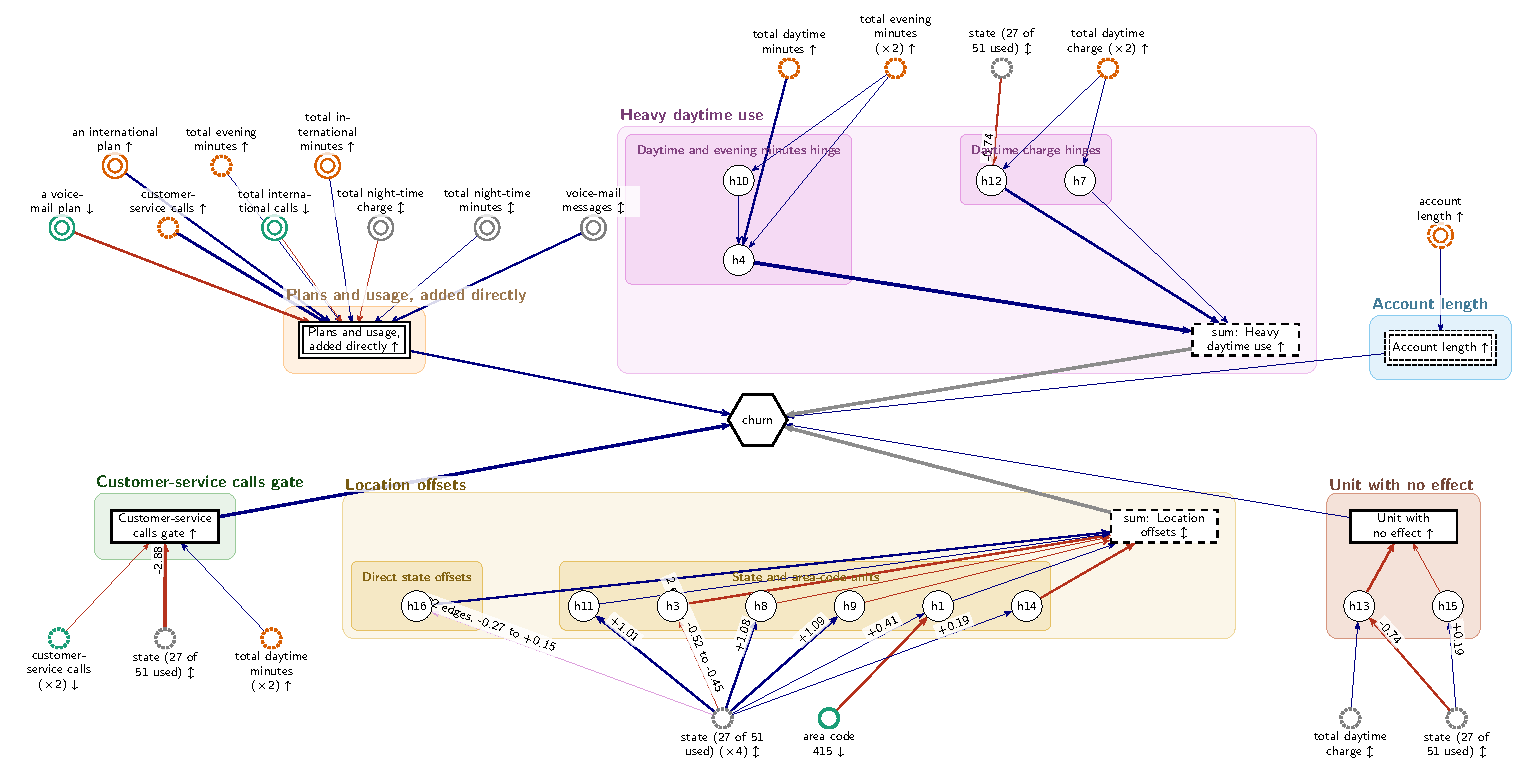
\includegraphics[trim={0.0bp 0 820.1bp 0},clip,width=\textheight,height=0.78\textwidth,keepaspectratio]{figures/exp2/networks/churn100-s4-explained}
  \caption{Churn, seed 4 (churn100-s4): every unit and connection of the explained model, nested by part. Shaded clusters are the 11 parts of the agent's explanation (8 leaf and 3 composition annotations, after 12 node splits and 2 identity nodes) and darker boxes the parts inside them; circles are hidden units; each cluster's rectangle is its output, a dashed `sum' an addition the next unit does; the hexagon is the model's output. An input used by several parts is drawn under each of them (dotted outline). Blue: positive weight (raises the score); red: negative weight (lowers it); thicker: larger weight. Orange outline and up arrow: raises the final prediction; teal and down arrow: lowers it; grey and double arrow: depends. Drawn in 2 pieces, left to right, on this and the next page.}
  \label{fig:exp2-net-churn100-s4-explained}
\end{sidewaysfigure}
\clearpage
\begin{sidewaysfigure}
  \centering
  \ContinuedFloat
  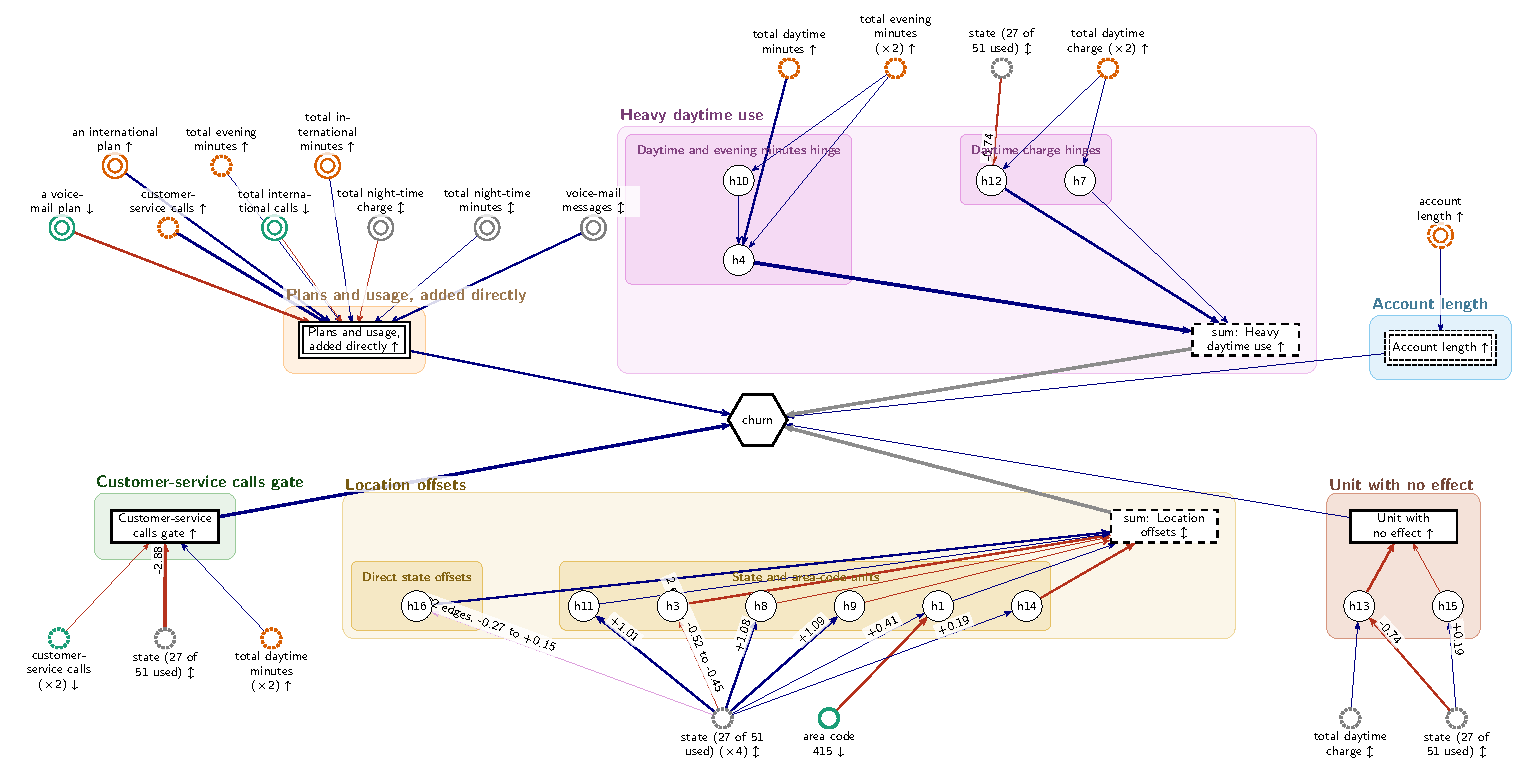
\includegraphics[trim={820.1bp 0 0.0bp 0},clip,width=\textheight,height=0.78\textwidth,keepaspectratio]{figures/exp2/networks/churn100-s4-explained}
  \caption[]{(continued, piece 2 of 2).}
\end{sidewaysfigure}

\clearpage
% Generated by thesis/ch7/exp2/networks.py -- do not edit by hand.
\begin{sidewaysfigure}
  \centering
  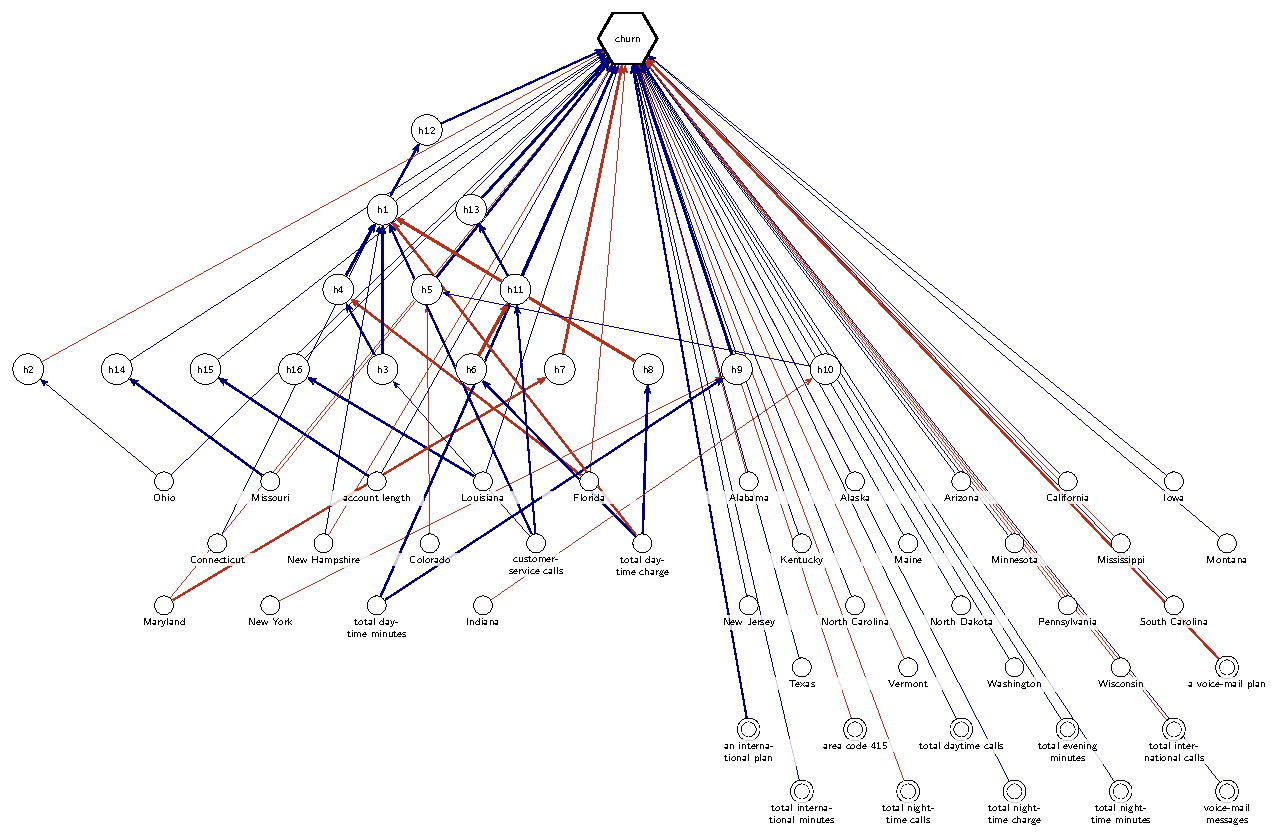
\includegraphics[width=\textheight,height=0.78\textwidth,keepaspectratio]{figures/exp2/networks/churn100-s5-raw}
  \caption{Churn, seed 5 (churn100-s5): the network as trained, before any explanation, in full. Inputs at the bottom (every input column its own node), hidden units by depth, the output at the top; 44 of 71 input columns are connected, with 16 hidden units and 75 enabled connections. Blue: positive weight (raises the score); red: negative weight (lowers it); thicker: larger weight. Orange outline and up arrow: raises the final prediction; teal and down arrow: lowers it; grey and double arrow: depends. Not used (no connection; 27 columns): Georgia, Hawaii, Idaho, Illinois, Kansas, Massachusetts, Arkansas, Michigan, Nebraska, New Mexico, Nevada, Oklahoma, Oregon, Rhode Island, South Dakota, Tennessee, Utah, Virginia, West Virginia, Wyoming, Washington DC, Delaware, area code 408, area code 510, total evening calls, total evening charge and total international charge.}
  \label{fig:exp2-net-churn100-s5-raw}
\end{sidewaysfigure}

\clearpage
% Generated by thesis/ch7/exp2/networks.py -- do not edit by hand.
\ifdefined\netfigheight\else\newlength{\netfigheight}\setlength{\netfigheight}{0.9\textwidth}\fi
\begin{sidewaysfigure}
  \centering
  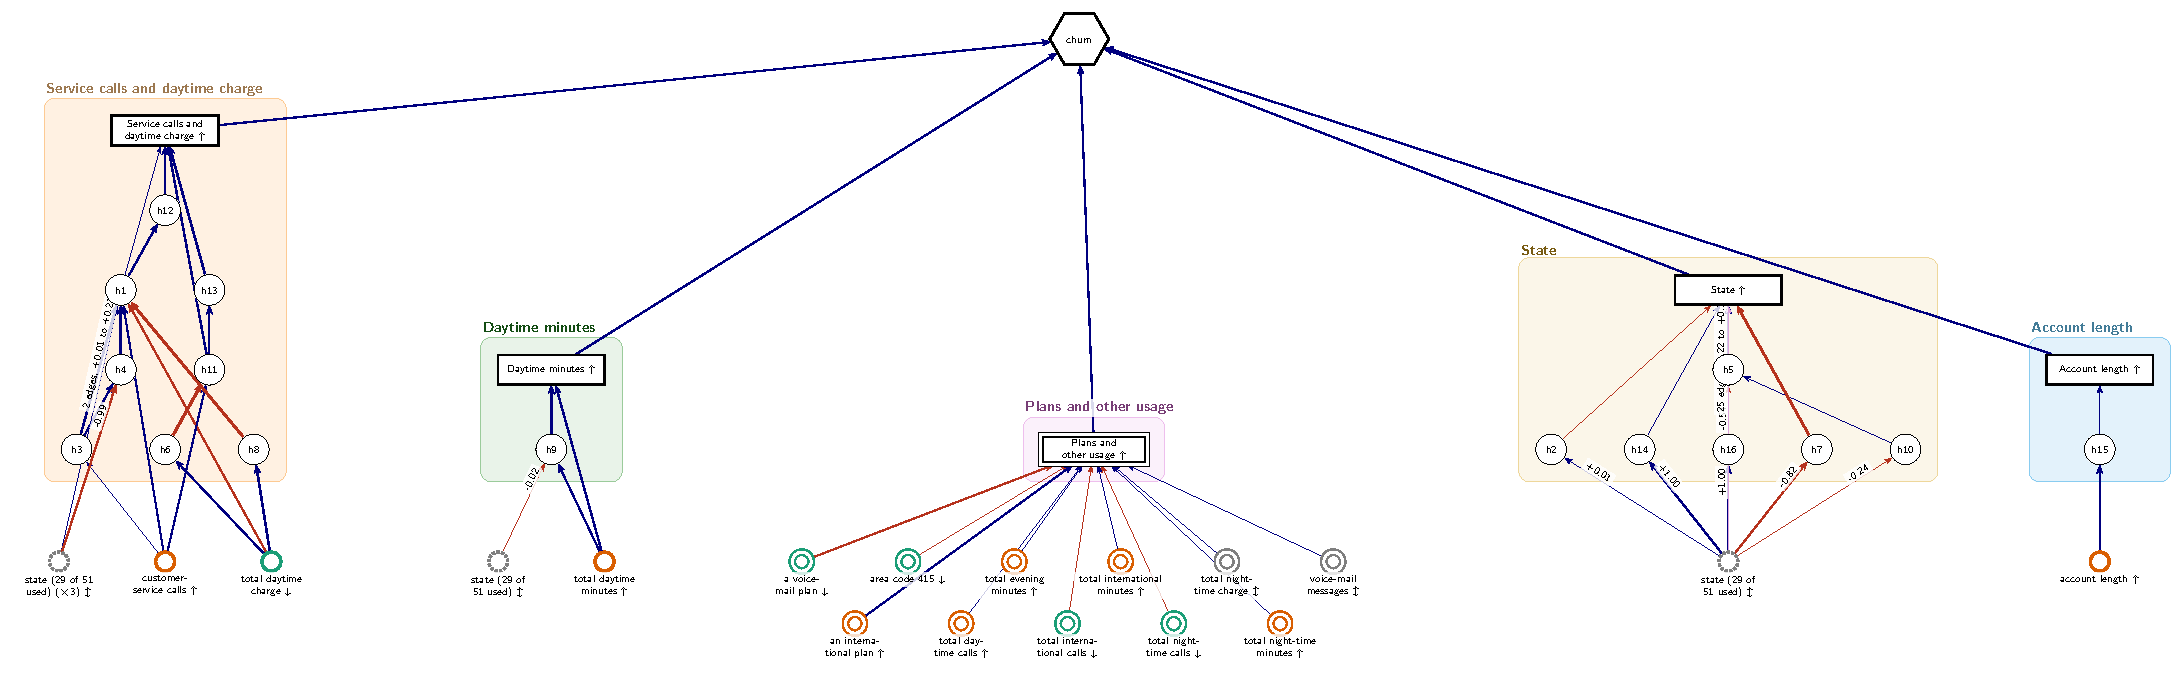
\includegraphics[width=\textheight,height=\netfigheight,keepaspectratio]{figures/exp2/networks/churn100-s5-explained}
  \caption{Churn, seed 5: the explained network, every unit nested by part.}
  \label{fig:exp2-net-churn100-s5-explained}
\end{sidewaysfigure}

\clearpage
% Generated by thesis/ch7/exp2/networks.py -- do not edit by hand.
\begin{sidewaysfigure}
  \centering
  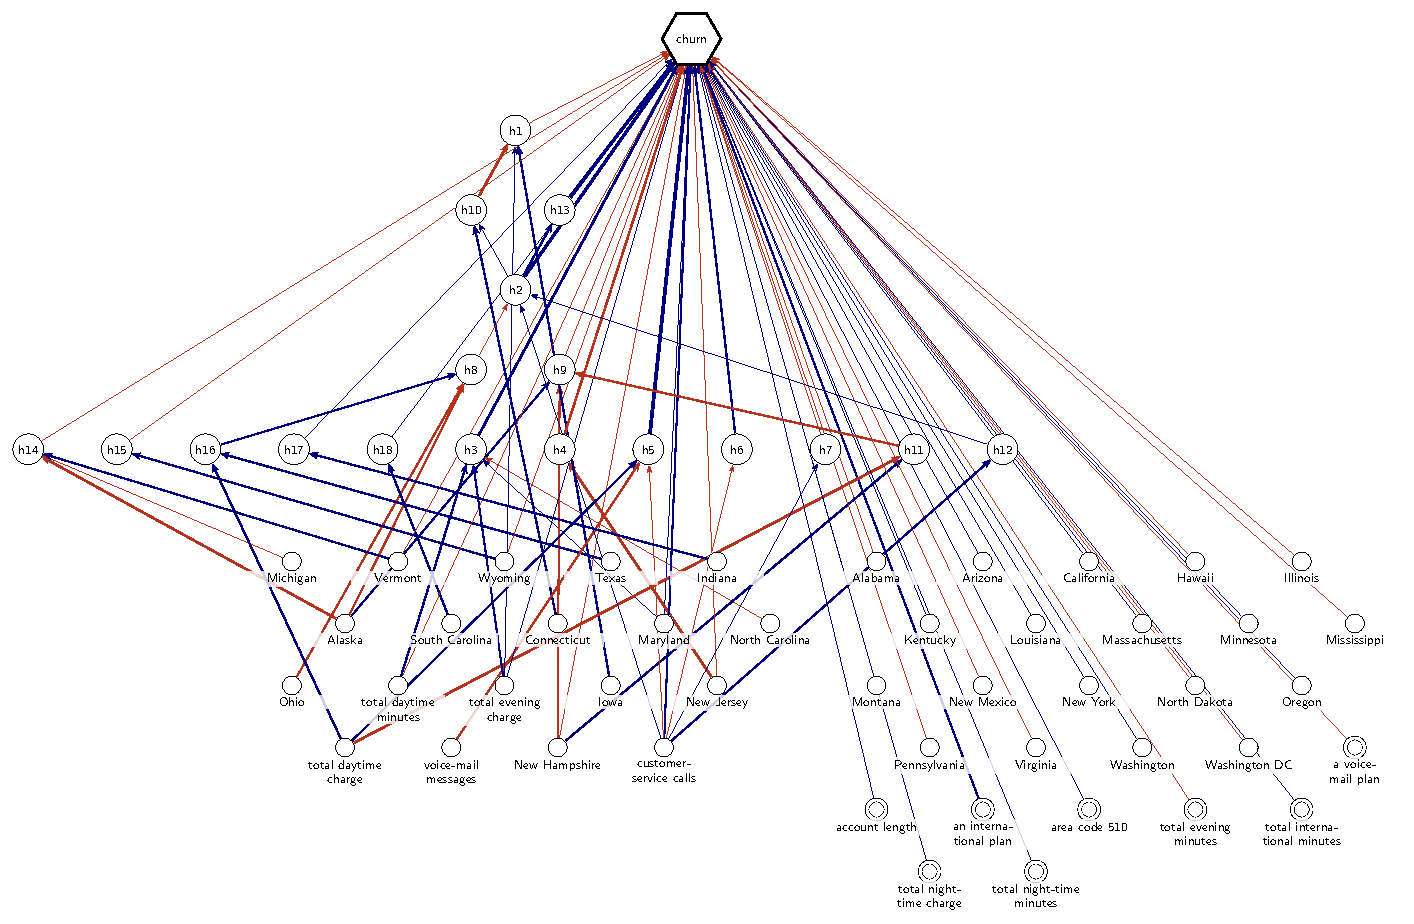
\includegraphics[width=\textheight,height=0.78\textwidth,keepaspectratio]{figures/exp2/networks/churn100-s6-raw}
  \caption{Churn, seed 6 (churn100-s6): the network as trained, before any explanation, in full. Inputs at the bottom (every input column its own node), hidden units by depth, the output at the top; 46 of 71 input columns are connected, with 18 hidden units and 84 enabled connections. Blue: positive weight (raises the score); red: negative weight (lowers it); thicker: larger weight. Orange outline and up arrow: raises the final prediction; teal and down arrow: lowers it; grey and double arrow: depends. Not used (no connection; 25 columns): Georgia, Idaho, Kansas, Arkansas, Maine, Missouri, Nebraska, Nevada, Oklahoma, Rhode Island, South Dakota, Tennessee, Utah, Wisconsin, West Virginia, Colorado, Delaware, Florida, area code 408, area code 415, total daytime calls, total evening calls, total night-time calls, total international calls and total international charge.}
  \label{fig:exp2-net-churn100-s6-raw}
\end{sidewaysfigure}

\clearpage
% Generated by thesis/ch7/exp2/networks.py -- do not edit by hand.
\ifdefined\netfigheight\else\newlength{\netfigheight}\setlength{\netfigheight}{0.9\textwidth}\fi
\begin{sidewaysfigure}
  \centering
  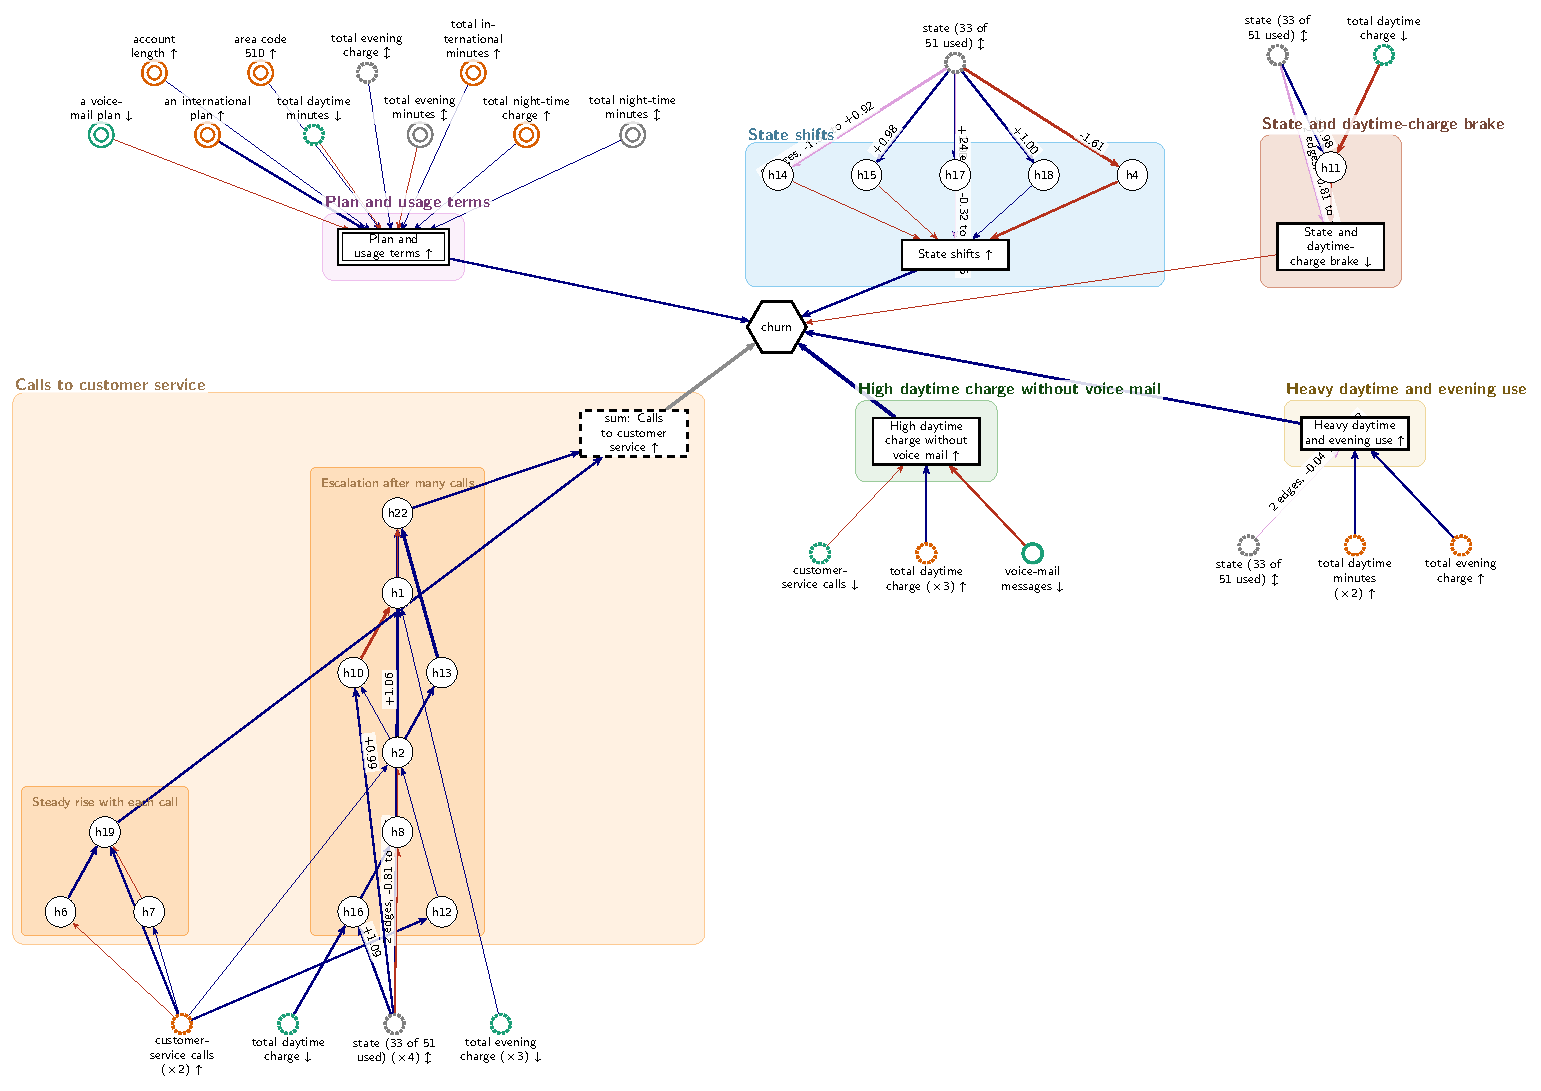
\includegraphics[width=\textheight,height=\netfigheight,keepaspectratio]{figures/exp2/networks/churn100-s6-explained}
  \caption{Churn, seed 6: the explained network, every unit nested by part.}
  \label{fig:exp2-net-churn100-s6-explained}
\end{sidewaysfigure}

\clearpage
% Generated by thesis/ch7/exp2/networks.py -- do not edit by hand.
\begin{sidewaysfigure}
  \centering
  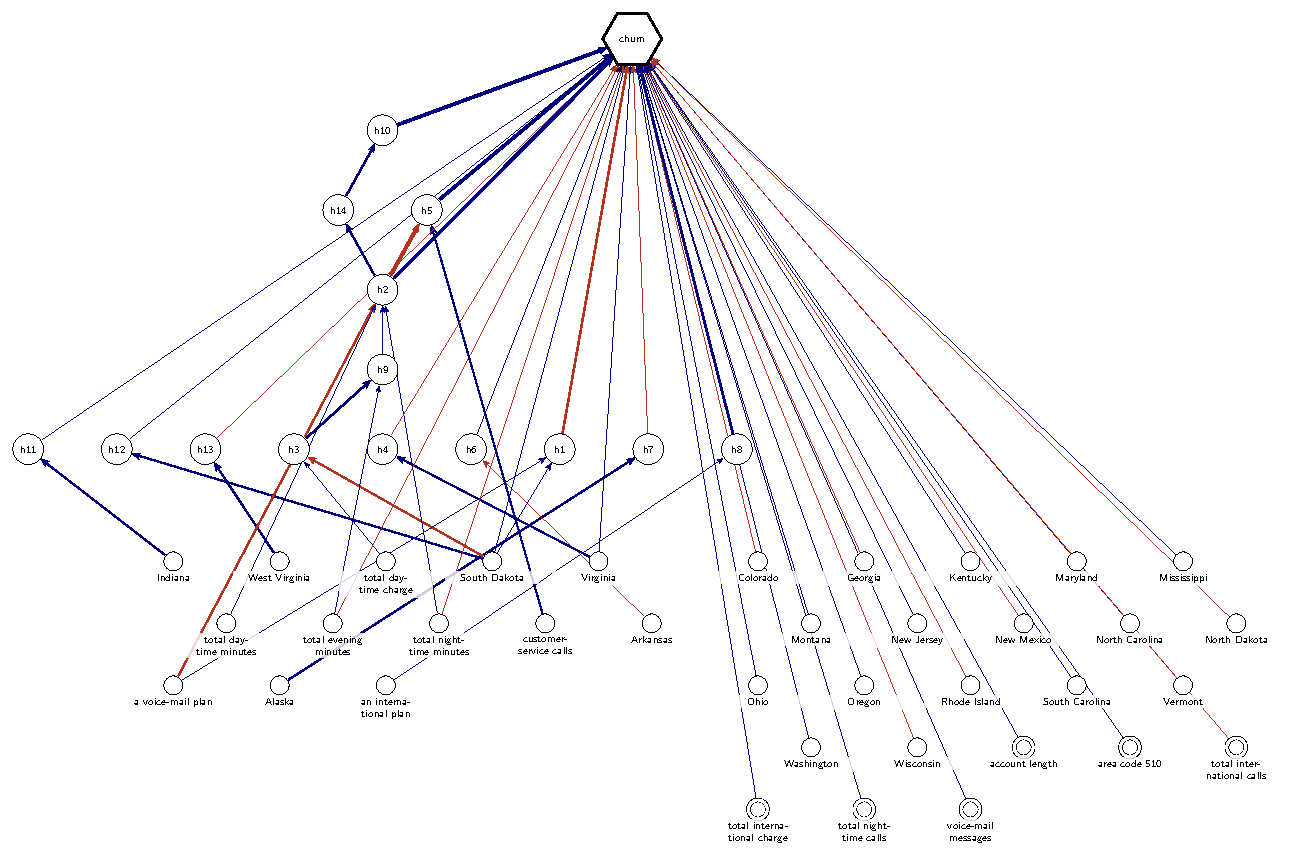
\includegraphics[width=\textheight,height=0.78\textwidth,keepaspectratio]{figures/exp2/networks/churn100-s7-raw}
  \caption{Churn, seed 7 (churn100-s7): the network as trained, before any explanation, in full. Inputs at the bottom (every input column its own node), hidden units by depth, the output at the top; 36 of 71 input columns are connected, with 14 hidden units and 59 enabled connections. Blue: positive weight (raises the score); red: negative weight (lowers it); thicker: larger weight. Orange outline and up arrow: raises the final prediction; teal and down arrow: lowers it; grey and double arrow: depends. Not used (no connection; 35 columns): Alabama, Hawaii, Iowa, Idaho, Illinois, Kansas, Louisiana, Massachusetts, Maine, Michigan, Minnesota, Missouri, Nebraska, Arizona, New Hampshire, Nevada, New York, Oklahoma, Pennsylvania, California, Tennessee, Texas, Utah, Wyoming, Connecticut, Washington DC, Delaware, Florida, area code 408, area code 415, total daytime calls, total evening calls, total evening charge, total night-time charge and total international minutes.}
  \label{fig:exp2-net-churn100-s7-raw}
\end{sidewaysfigure}

\clearpage
% Generated by thesis/ch7/exp2/networks.py -- do not edit by hand.
\begin{sidewaysfigure}
  \centering
  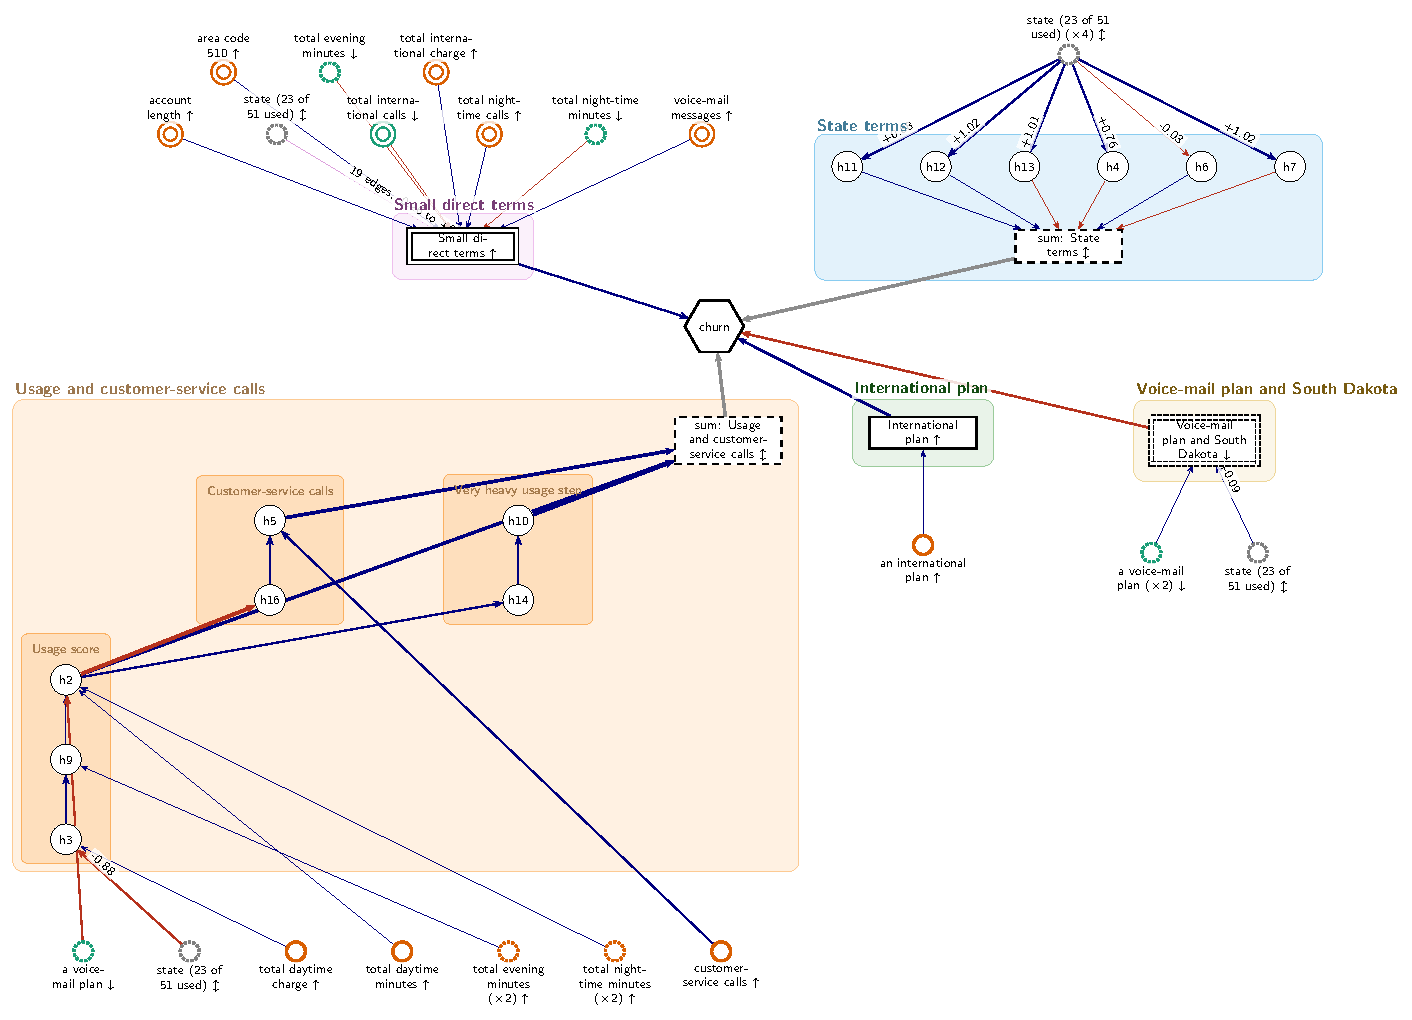
\includegraphics[trim={0.0bp 0 692.6bp 0},clip,width=\textheight,height=0.78\textwidth,keepaspectratio]{figures/exp2/networks/churn100-s7-explained}
  \caption{Churn, seed 7 (churn100-s7): every unit and connection of the explained model, nested by part. Shaded clusters are the 9 parts of the agent's explanation (7 leaf and 2 composition annotations, after 5 node splits and 2 identity nodes) and darker boxes the parts inside them; circles are hidden units; each cluster's rectangle is its output, a dashed `sum' an addition the next unit does; the hexagon is the model's output. An input used by several parts is drawn under each of them (dotted outline). Blue: positive weight (raises the score); red: negative weight (lowers it); thicker: larger weight. Orange outline and up arrow: raises the final prediction; teal and down arrow: lowers it; grey and double arrow: depends. Drawn in 2 pieces, left to right, on this and the next page.}
  \label{fig:exp2-net-churn100-s7-explained}
\end{sidewaysfigure}
\clearpage
\begin{sidewaysfigure}
  \centering
  \ContinuedFloat
  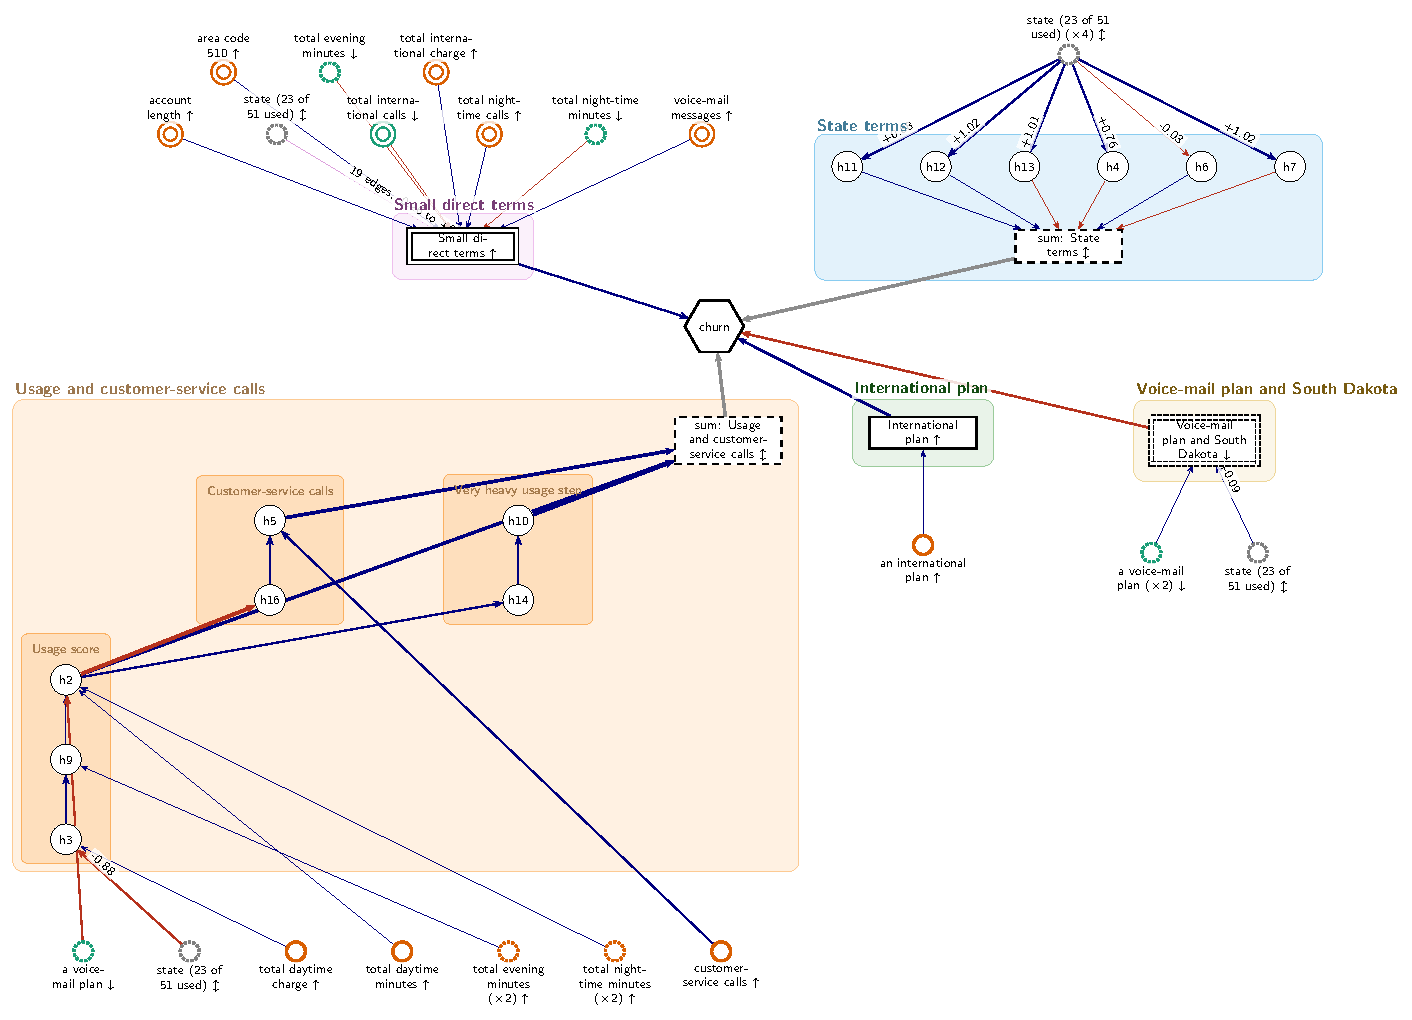
\includegraphics[trim={692.6bp 0 0.0bp 0},clip,width=\textheight,height=0.78\textwidth,keepaspectratio]{figures/exp2/networks/churn100-s7-explained}
  \caption[]{(continued, piece 2 of 2).}
\end{sidewaysfigure}

\clearpage
% Generated by thesis/ch7/exp2/networks.py -- do not edit by hand.
\begin{sidewaysfigure}
  \centering
  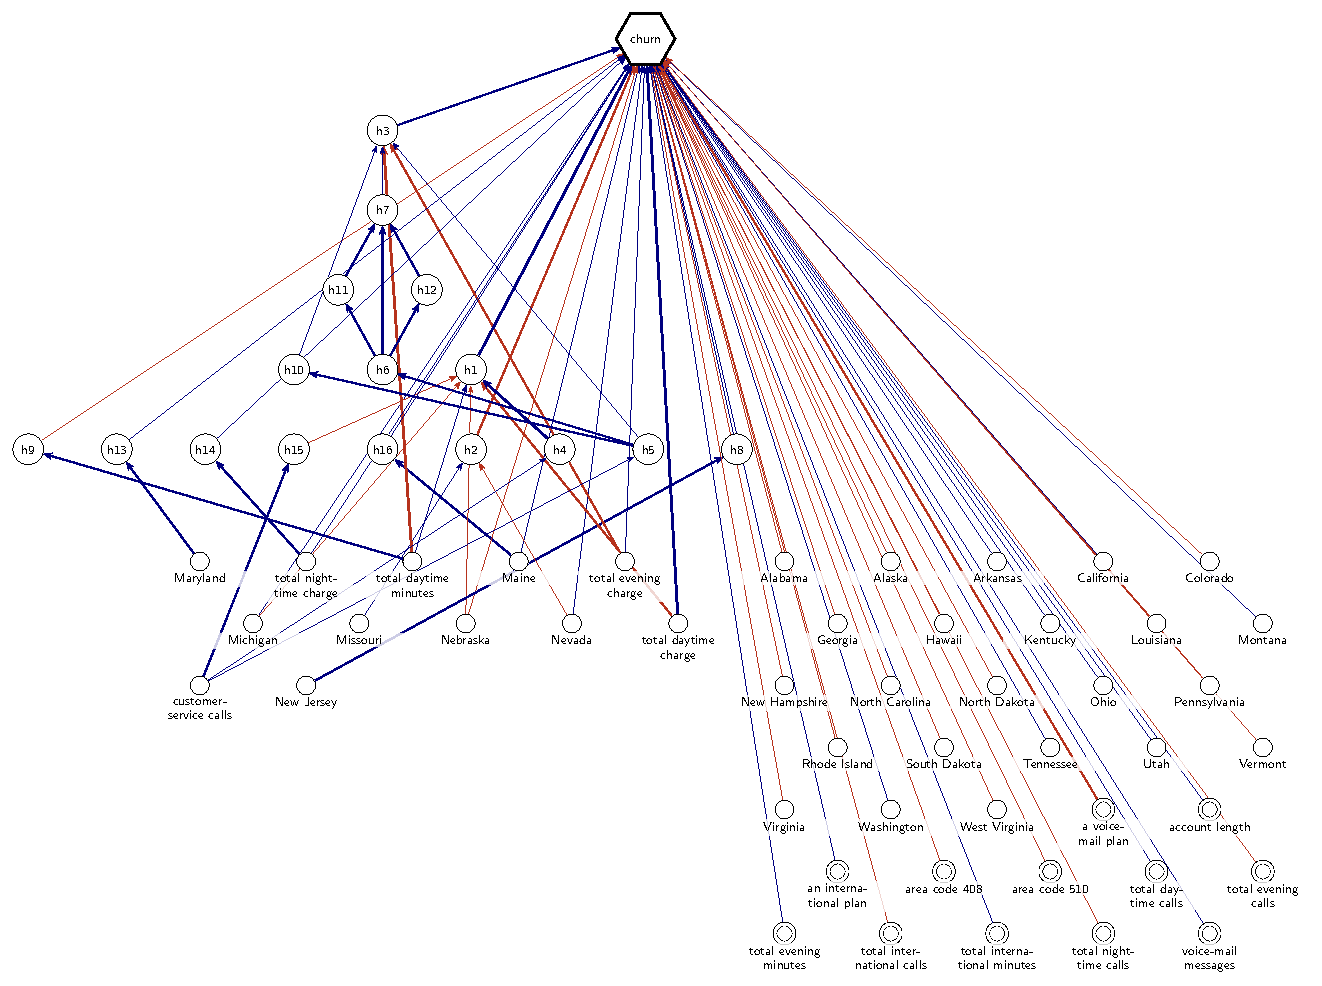
\includegraphics[width=\textheight,height=0.78\textwidth,keepaspectratio]{figures/exp2/networks/churn100-s8-raw}
  \caption{Churn, seed 8 (churn100-s8): the network as trained, before any explanation, in full. Inputs at the bottom (every input column its own node), hidden units by depth, the output at the top; 47 of 71 input columns are connected, with 16 hidden units and 79 enabled connections. Blue: positive weight (raises the score); red: negative weight (lowers it); thicker: larger weight. Orange outline and up arrow: raises the final prediction; teal and down arrow: lowers it; grey and double arrow: depends. Not used (no connection; 24 columns): Iowa, Idaho, Illinois, Indiana, Kansas, Massachusetts, Minnesota, Mississippi, Arizona, New Mexico, New York, Oklahoma, Oregon, South Carolina, Texas, Wisconsin, Wyoming, Connecticut, Washington DC, Delaware, Florida, area code 415, total night-time minutes and total international charge.}
  \label{fig:exp2-net-churn100-s8-raw}
\end{sidewaysfigure}

\clearpage
% Generated by thesis/ch7/exp2/networks.py -- do not edit by hand.
\ifdefined\netfigheight\else\newlength{\netfigheight}\setlength{\netfigheight}{0.9\textwidth}\fi
\begin{sidewaysfigure}
  \centering
  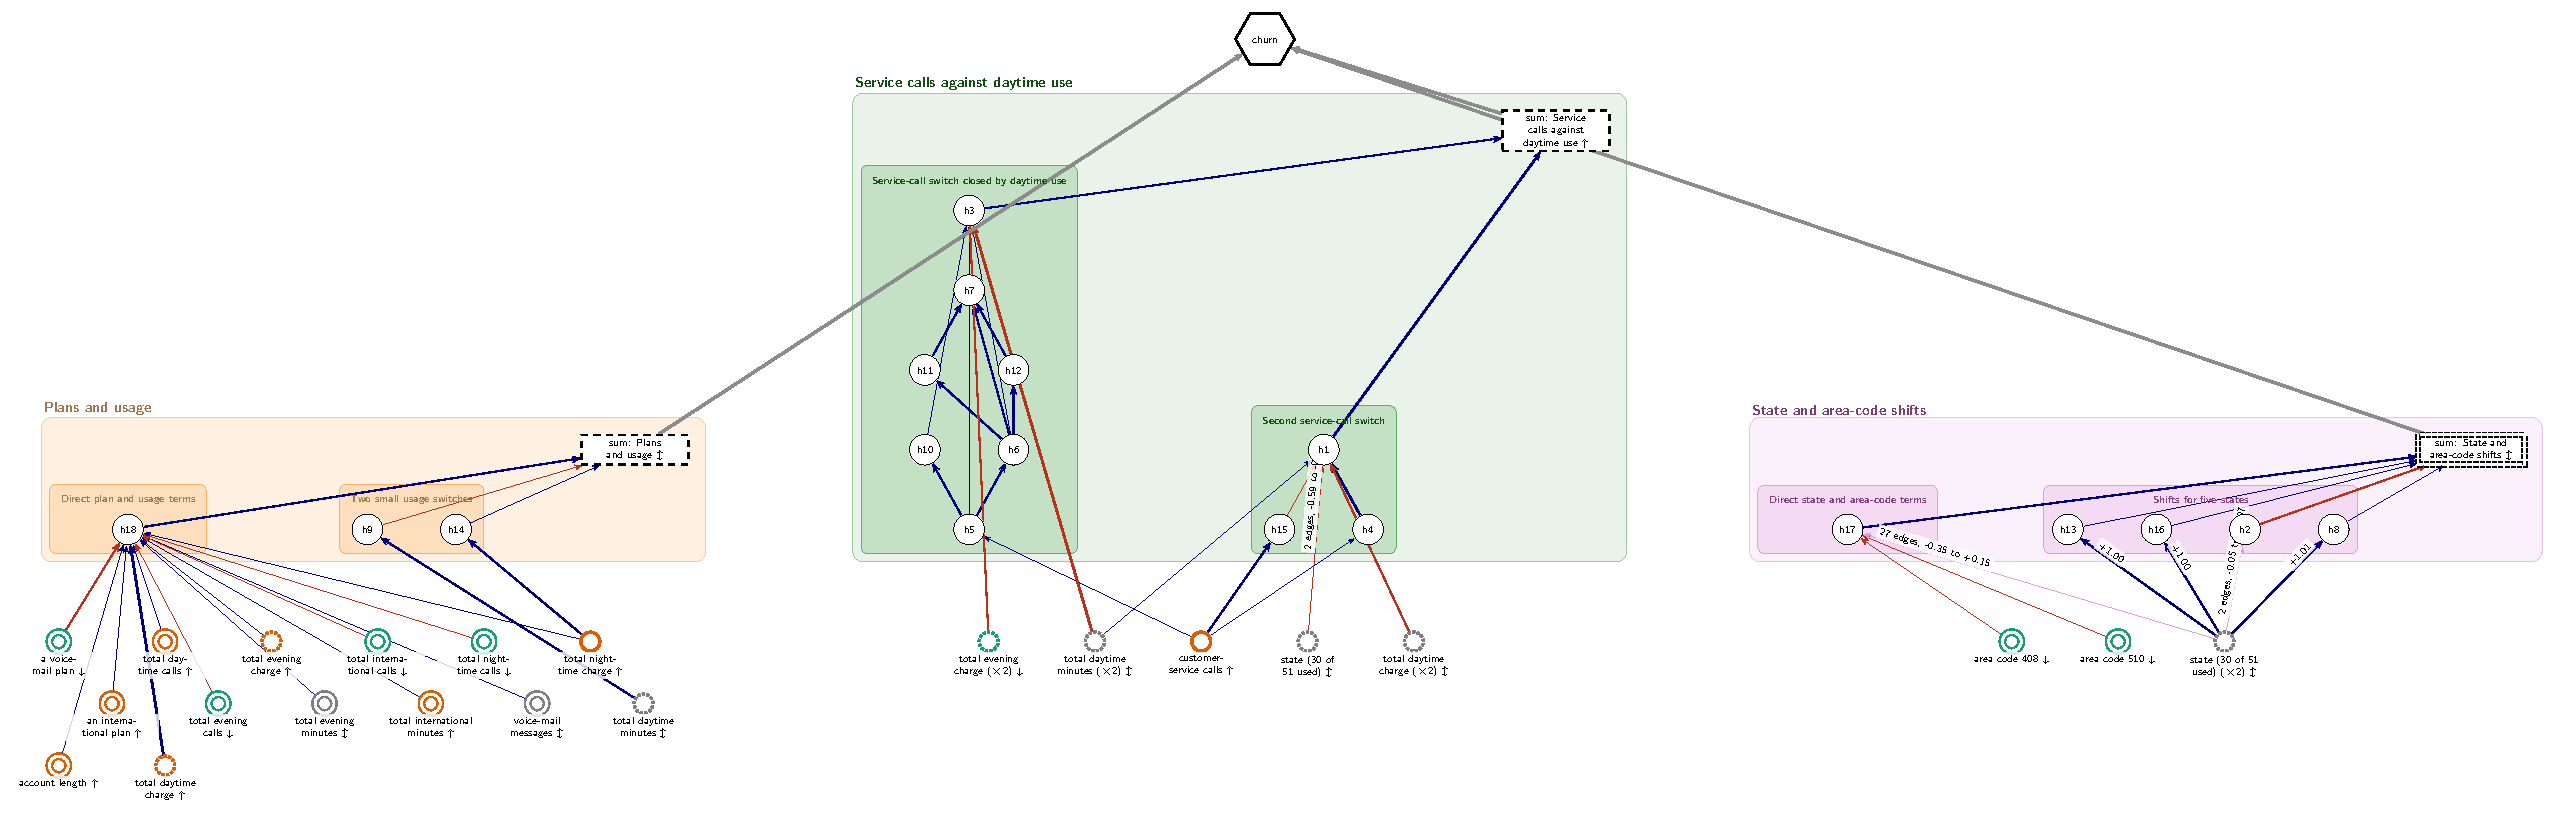
\includegraphics[width=\textheight,height=\netfigheight,keepaspectratio]{figures/exp2/networks/churn100-s8-explained}
  \caption{Churn, seed 8: the explained network, every unit nested by part.}
  \label{fig:exp2-net-churn100-s8-explained}
\end{sidewaysfigure}

\clearpage
% Generated by thesis/ch7/exp2/networks.py -- do not edit by hand.
\begin{sidewaysfigure}
  \centering
  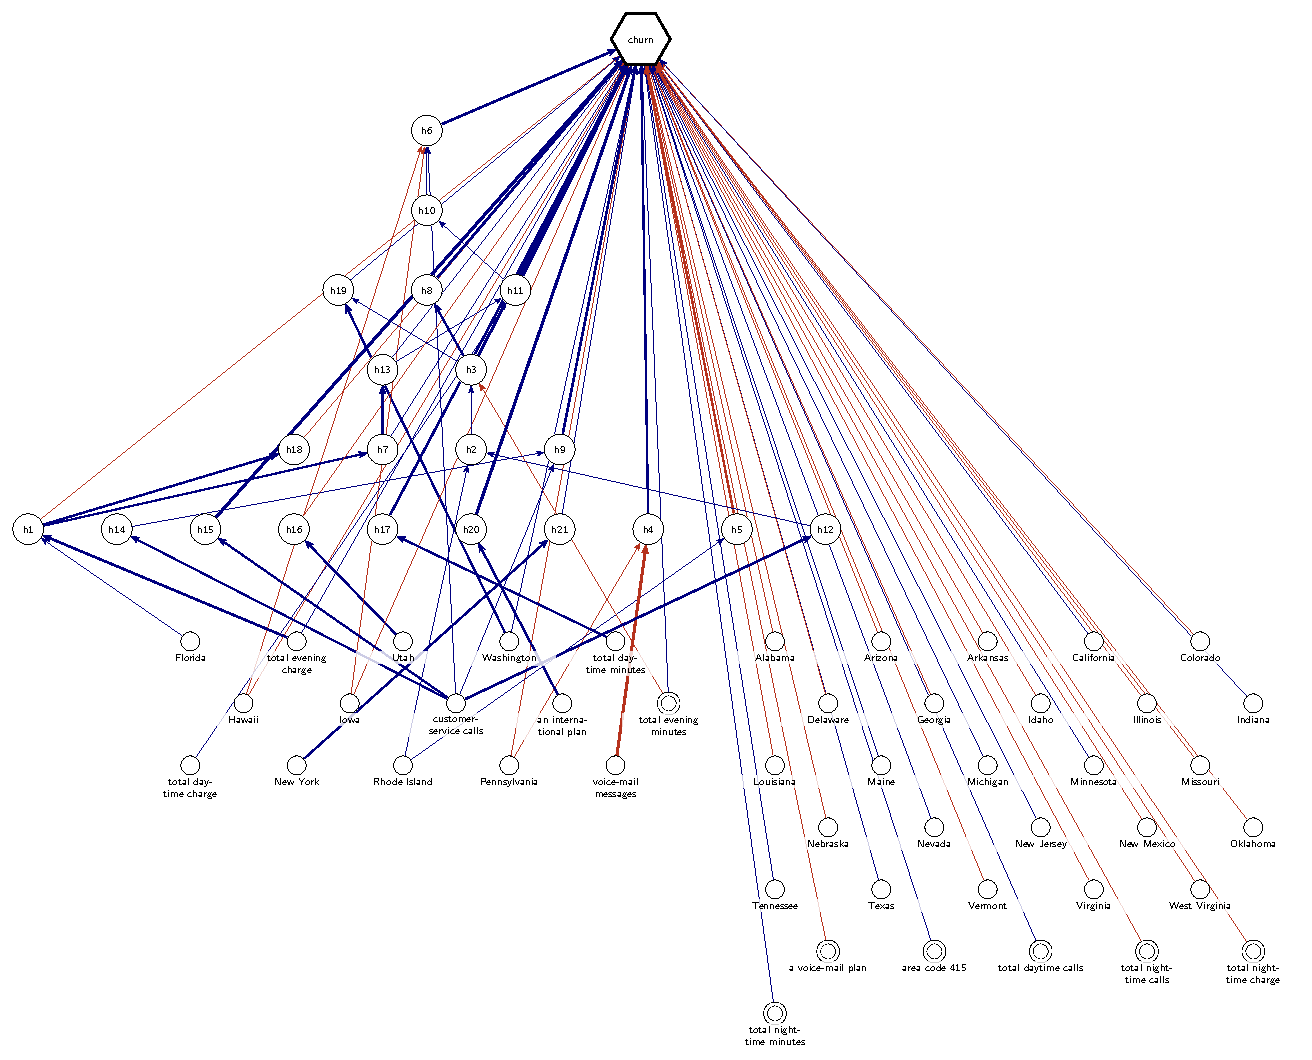
\includegraphics[width=\textheight,height=0.78\textwidth,keepaspectratio]{figures/exp2/networks/churn100-s9-raw}
  \caption{Churn, seed 9 (churn100-s9): the network as trained, before any explanation, in full. Inputs at the bottom (every input column its own node), hidden units by depth, the output at the top; 46 of 71 input columns are connected, with 21 hidden units and 85 enabled connections. Blue: positive weight (raises the score); red: negative weight (lowers it); thicker: larger weight. Orange outline and up arrow: raises the final prediction; teal and down arrow: lowers it; grey and double arrow: depends. Not used (no connection; 25 columns): Alaska, Kansas, Kentucky, Massachusetts, Maryland, Mississippi, Montana, North Carolina, North Dakota, New Hampshire, Ohio, Oregon, South Carolina, South Dakota, Wisconsin, Wyoming, Connecticut, Washington DC, account length, area code 408, area code 510, total evening calls, total international minutes, total international calls and total international charge.}
  \label{fig:exp2-net-churn100-s9-raw}
\end{sidewaysfigure}

\clearpage
% Generated by thesis/ch7/exp2/networks.py -- do not edit by hand.
\begin{sidewaysfigure}
  \centering
  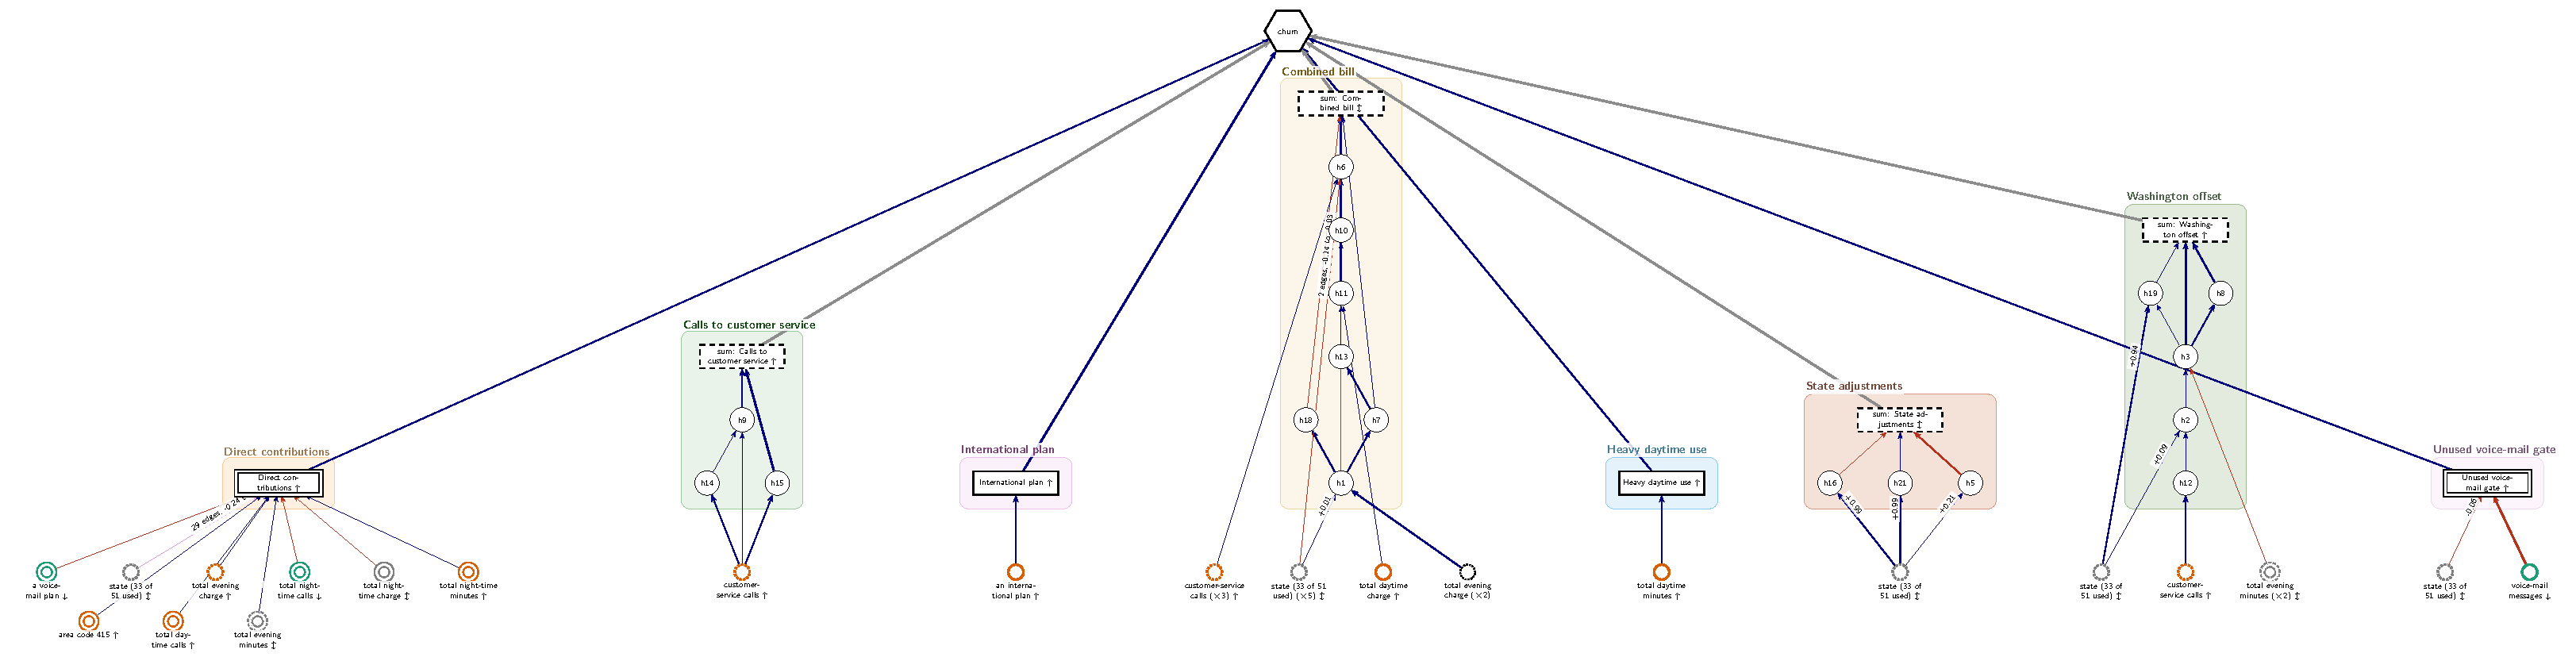
\includegraphics[trim={0.0bp 0 767.1bp 0},clip,width=\textheight,height=0.78\textwidth,keepaspectratio]{figures/exp2/networks/churn100-s9-explained}
  \caption{Churn, seed 9 (churn100-s9): every unit and connection of the explained model, nested by part. Shaded clusters are the 9 parts of the agent's explanation (8 leaf and 1 composition annotations, after 8 node splits and 1 identity nodes) and darker boxes the parts inside them; circles are hidden units; each cluster's rectangle is its output, a dashed `sum' an addition the next unit does; the hexagon is the model's output. An input used by several parts is drawn under each of them (dotted outline). Blue: positive weight (raises the score); red: negative weight (lowers it); thicker: larger weight. Orange outline and up arrow: raises the final prediction; teal and down arrow: lowers it; grey and double arrow: depends. Drawn in 2 pieces, left to right, on this and the next page.}
  \label{fig:exp2-net-churn100-s9-explained}
\end{sidewaysfigure}
\clearpage
\begin{sidewaysfigure}
  \centering
  \ContinuedFloat
  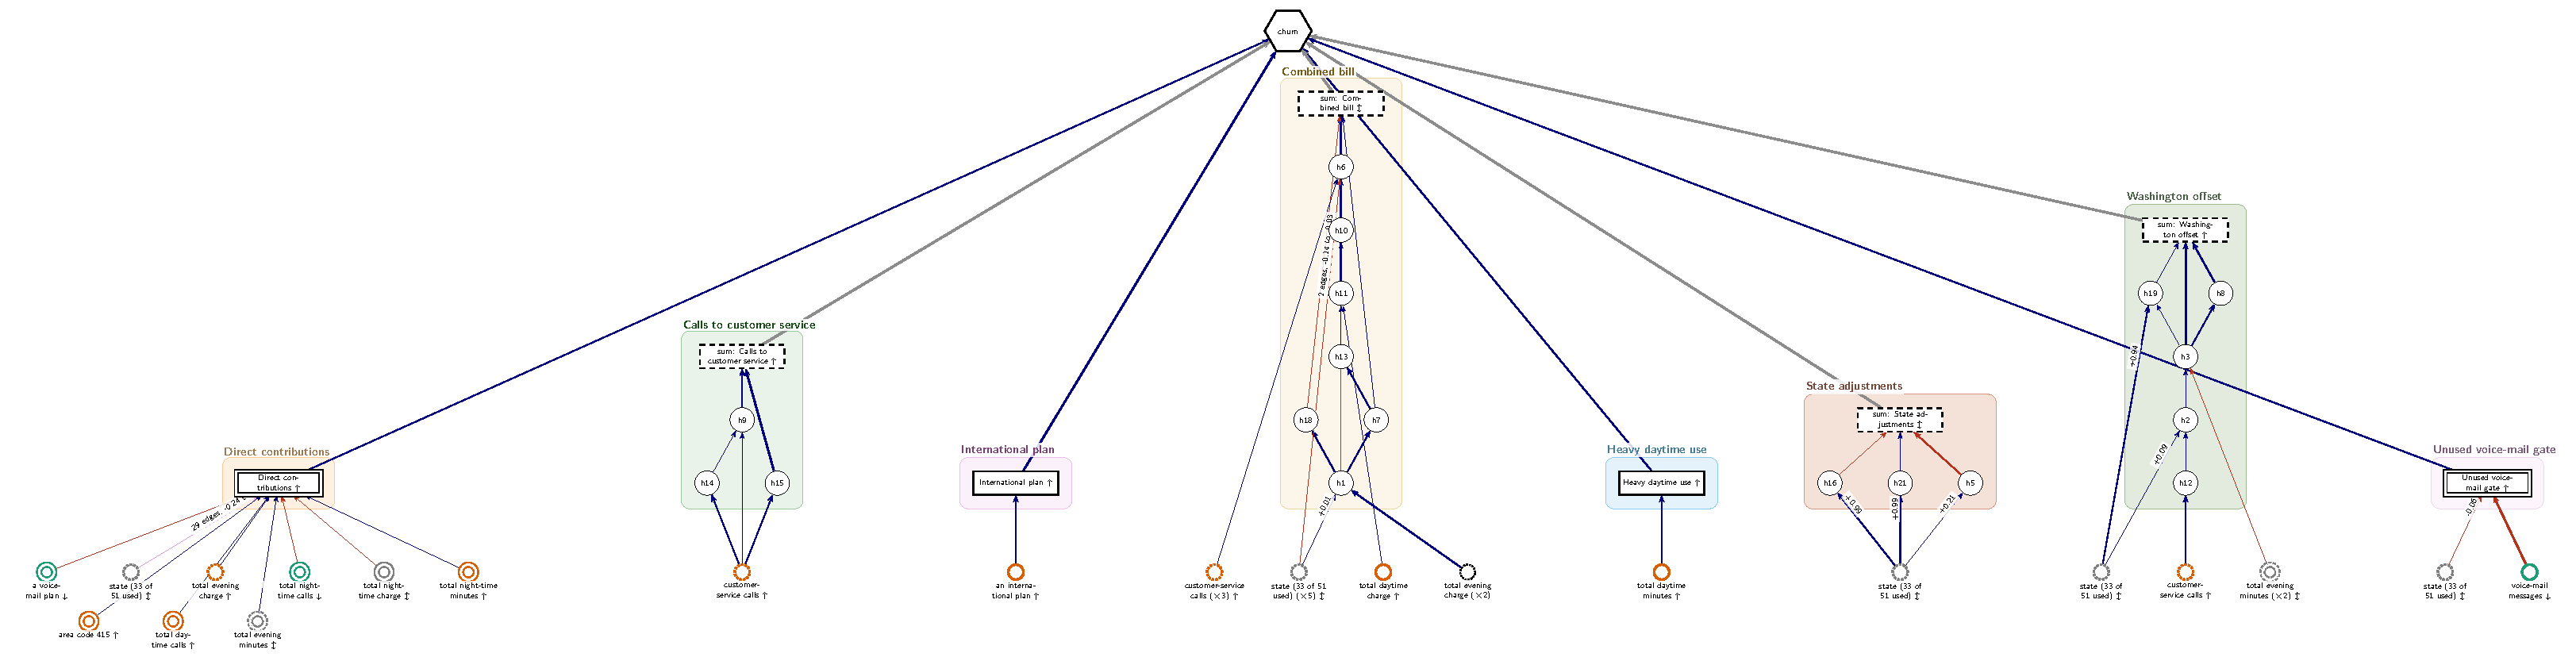
\includegraphics[trim={767.1bp 0 0.0bp 0},clip,width=\textheight,height=0.78\textwidth,keepaspectratio]{figures/exp2/networks/churn100-s9-explained}
  \caption[]{(continued, piece 2 of 2).}
\end{sidewaysfigure}

\clearpage
% Heart-100: the ten networks (the dataset is named in each caption)
% Generated by thesis/ch7/exp2/networks.py -- do not edit by hand.
\begin{sidewaysfigure}
  \centering
  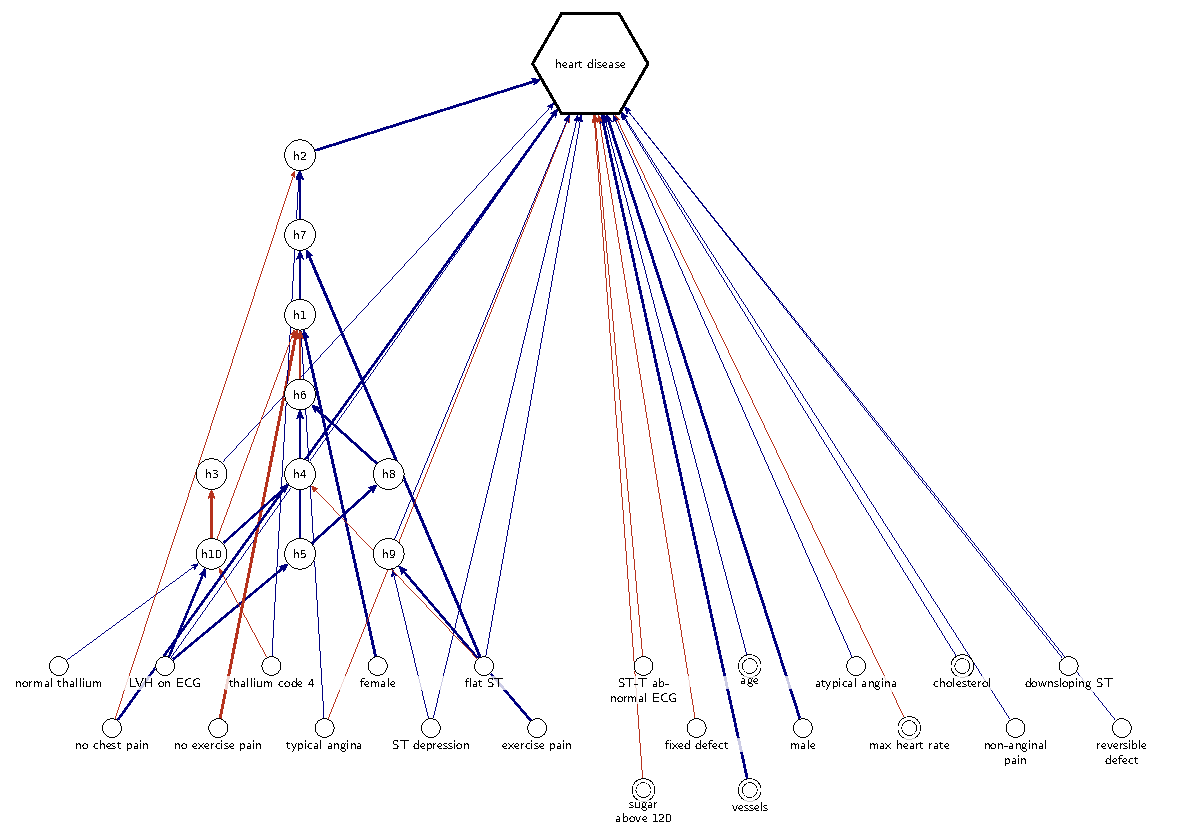
\includegraphics[width=\textheight,height=0.78\textwidth,keepaspectratio]{figures/exp2/networks/heart100-s0-raw}
  \caption{Heart-100, seed 0 (heart100-s0): the network as trained, before any explanation, in full. Inputs at the bottom (every input column its own node), hidden units by depth, the output at the top; 22 of 26 input columns are connected, with 10 hidden units and 43 enabled connections. Blue: positive weight (raises the score); red: negative weight (lowers it); thicker: larger weight. Orange outline and up arrow: raises the final prediction; teal and down arrow: lowers it; grey and double arrow: depends. Not used (no connection; 4 columns): blood pressure, sugar 120 or less, normal ECG and upsloping ST.}
  \label{fig:exp2-net-heart100-s0-raw}
\end{sidewaysfigure}

\clearpage
% Generated by thesis/ch7/exp2/networks.py -- do not edit by hand.
\begin{sidewaysfigure}
  \centering
  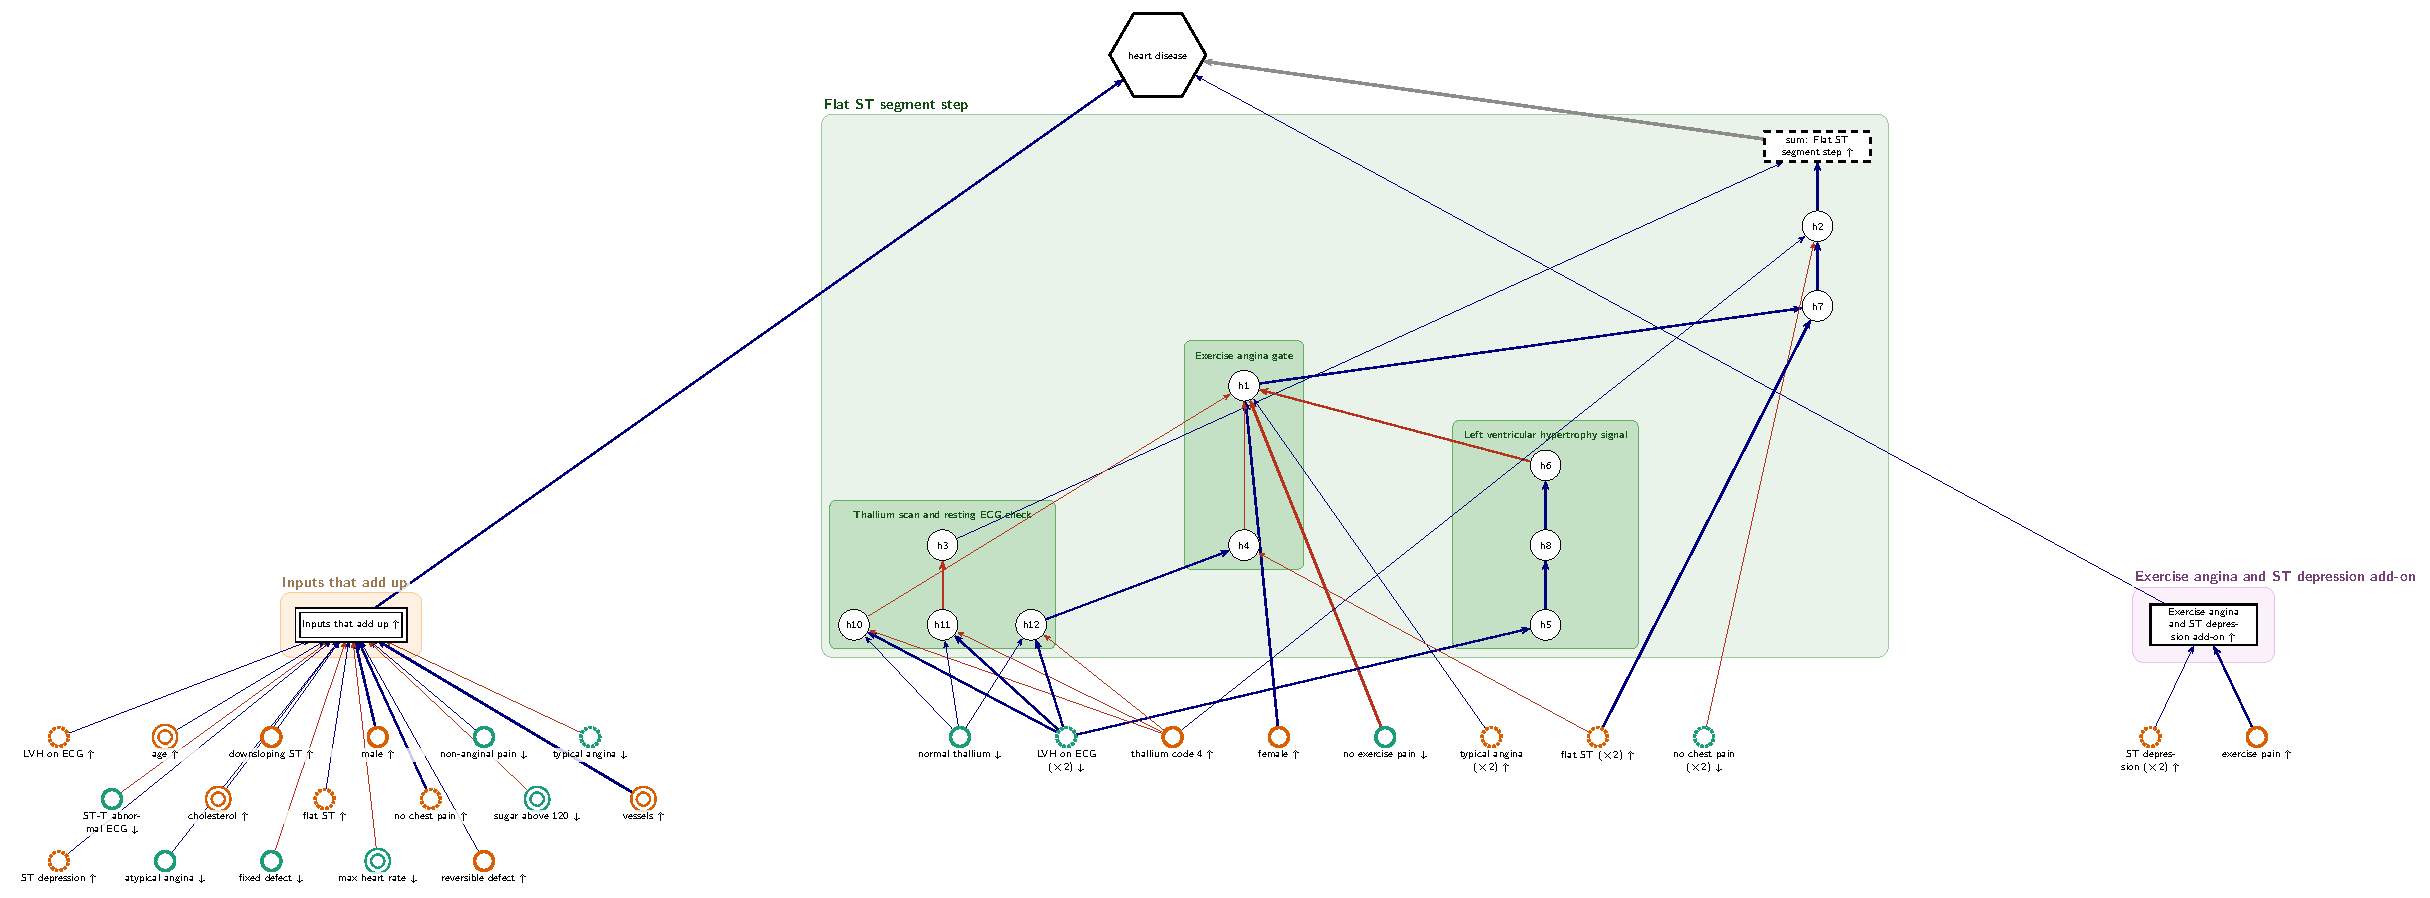
\includegraphics[width=\textheight,height=0.78\textwidth,keepaspectratio]{figures/exp2/networks/heart100-s0-explained}
  \caption{Heart-100, seed 0 (heart100-s0): every unit and connection of the explained model, nested by part. Shaded clusters are the 7 parts of the agent's explanation (4 leaf and 3 composition annotations, after 7 node splits and 1 identity nodes) and darker boxes the parts inside them; circles are hidden units; each cluster's rectangle is its output, a dashed `sum' an addition the next unit does; the hexagon is the model's output. An input used by several parts is drawn under each of them (dotted outline). Blue: positive weight (raises the score); red: negative weight (lowers it); thicker: larger weight. Orange outline and up arrow: raises the final prediction; teal and down arrow: lowers it; grey and double arrow: depends.}
  \label{fig:exp2-net-heart100-s0-explained}
\end{sidewaysfigure}

\clearpage
% Generated by thesis/ch7/exp2/networks.py -- do not edit by hand.
\ifdefined\netfigheight\else\newlength{\netfigheight}\setlength{\netfigheight}{0.9\textwidth}\fi
\begin{sidewaysfigure}
  \centering
  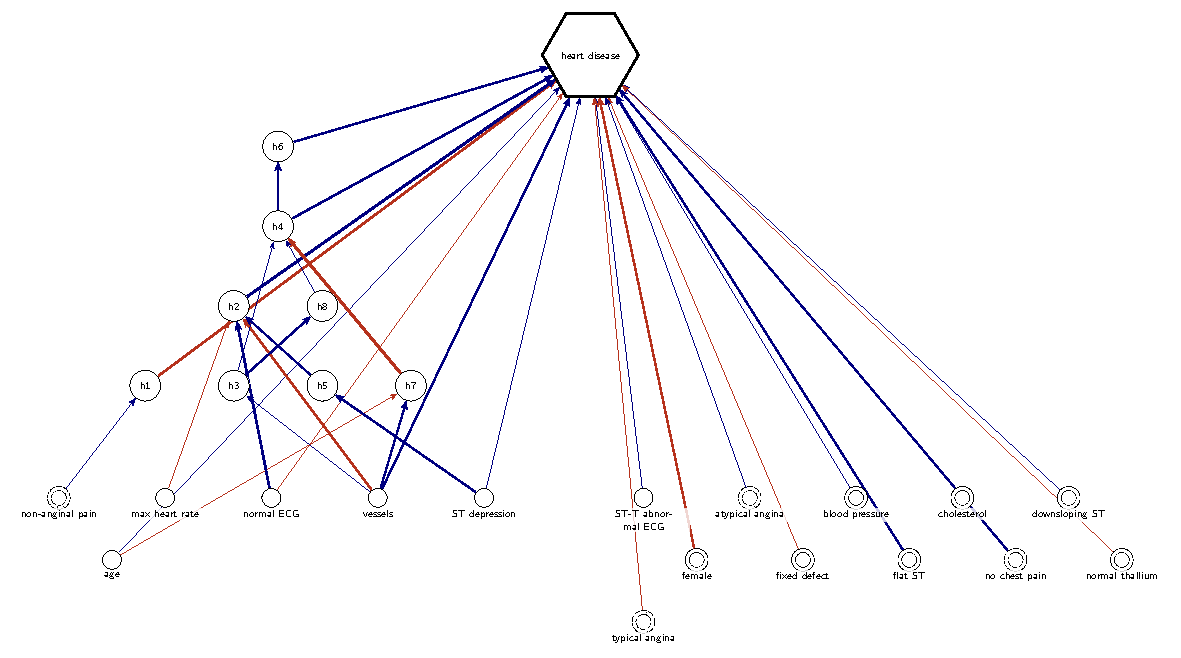
\includegraphics[width=\textheight,height=\netfigheight,keepaspectratio]{figures/exp2/networks/heart100-s1-raw}
  \caption{Heart-100, seed 1: the network as trained, before any explanation.}
  \label{fig:exp2-net-heart100-s1-raw}
\end{sidewaysfigure}

\clearpage
% Generated by thesis/ch7/exp2/networks.py -- do not edit by hand.
\begin{sidewaysfigure}
  \centering
  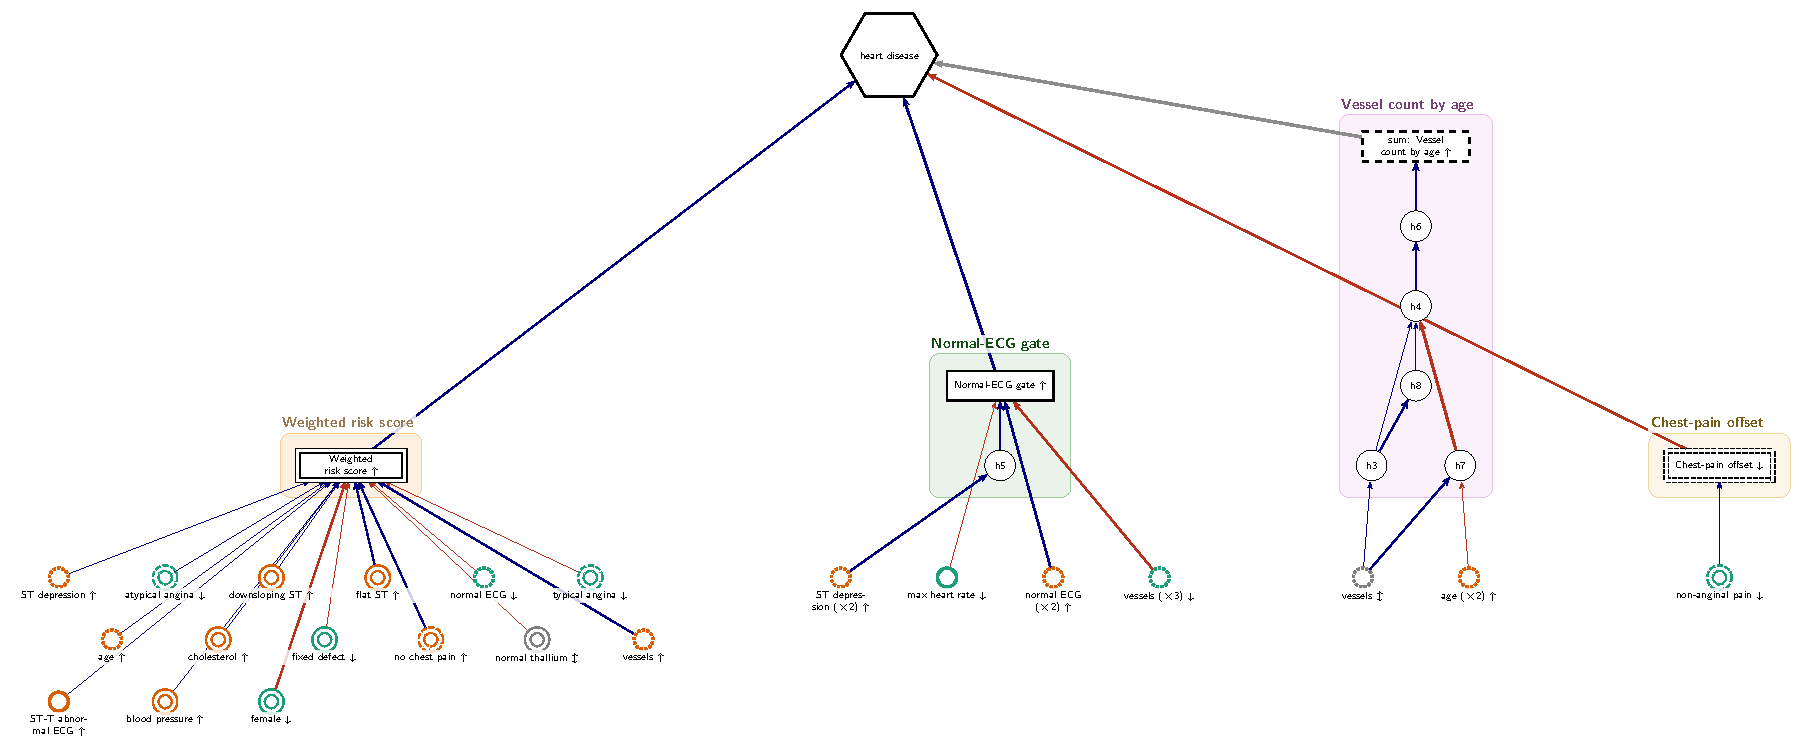
\includegraphics[width=\textheight,height=0.9\textwidth,keepaspectratio]{figures/exp2/networks/heart100-s1-explained}
  \caption{Heart-100, seed 1: the explained network, every unit nested by part.}
  \label{fig:exp2-net-heart100-s1-explained}
\end{sidewaysfigure}

\clearpage
% Generated by thesis/ch7/exp2/networks.py -- do not edit by hand.
\begin{sidewaysfigure}
  \centering
  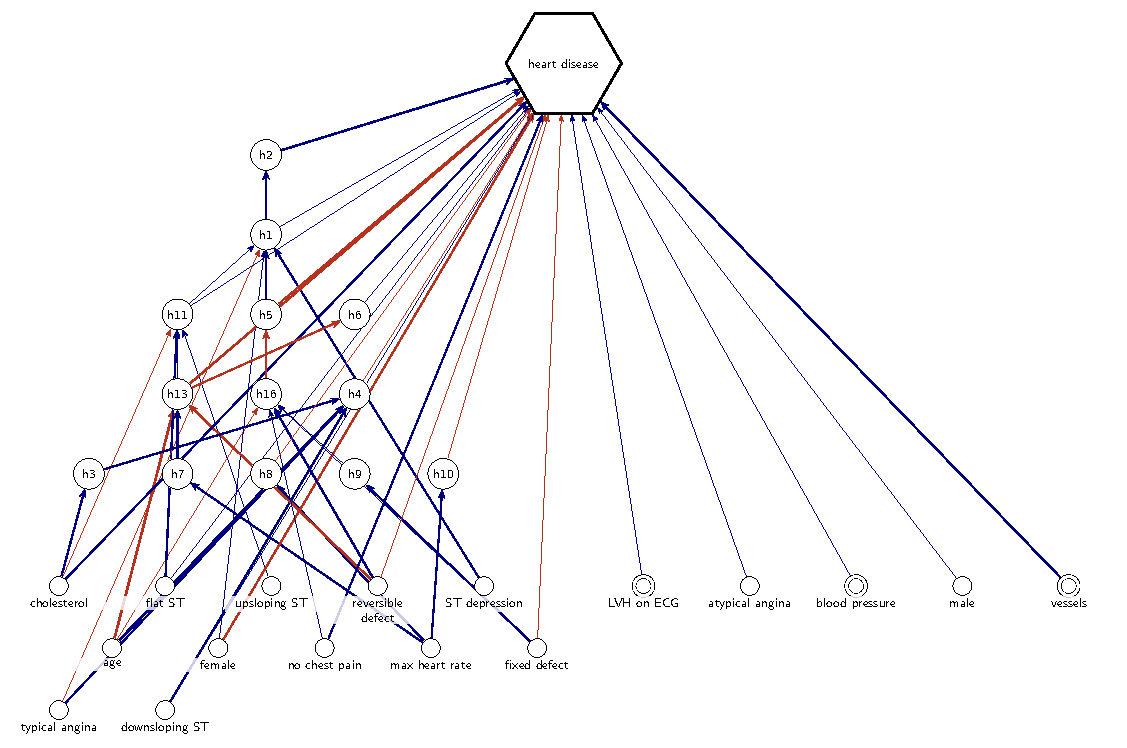
\includegraphics[width=\textheight,height=0.78\textwidth,keepaspectratio]{figures/exp2/networks/heart100-s2-raw}
  \caption{Heart-100, seed 2 (heart100-s2): the network as trained, before any explanation, in full. Inputs at the bottom (every input column its own node), hidden units by depth, the output at the top; 17 of 26 input columns are connected, with 13 hidden units and 50 enabled connections. Blue: positive weight (raises the score); red: negative weight (lowers it); thicker: larger weight. Orange outline and up arrow: raises the final prediction; teal and down arrow: lowers it; grey and double arrow: depends. Not used (no connection; 9 columns): non-anginal pain, sugar 120 or less, sugar above 120, normal ECG, ST-T abnormal ECG, no exercise pain, exercise pain, normal thallium and thallium code 4.}
  \label{fig:exp2-net-heart100-s2-raw}
\end{sidewaysfigure}

\clearpage
% Generated by thesis/ch7/exp2/networks.py -- do not edit by hand.
\begin{sidewaysfigure}
  \centering
  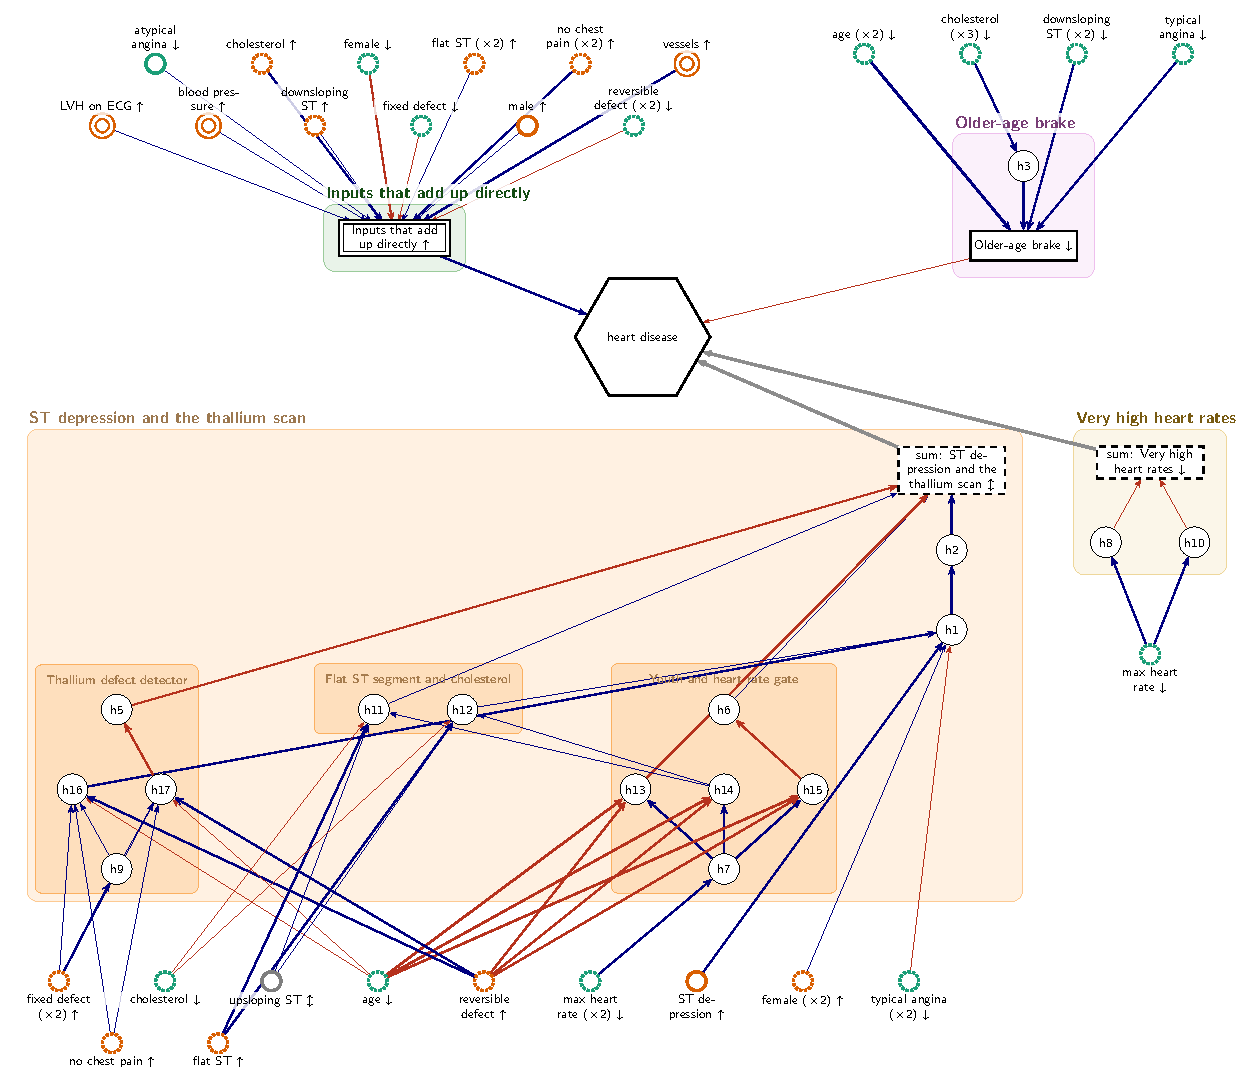
\includegraphics[width=\textheight,height=0.9\textwidth,keepaspectratio]{figures/exp2/networks/heart100-s2-explained}
  \caption{Heart-100, seed 2: the explained network, every unit nested by part.}
  \label{fig:exp2-net-heart100-s2-explained}
\end{sidewaysfigure}

\clearpage
% Generated by thesis/ch7/exp2/networks.py -- do not edit by hand.
\begin{sidewaysfigure}
  \centering
  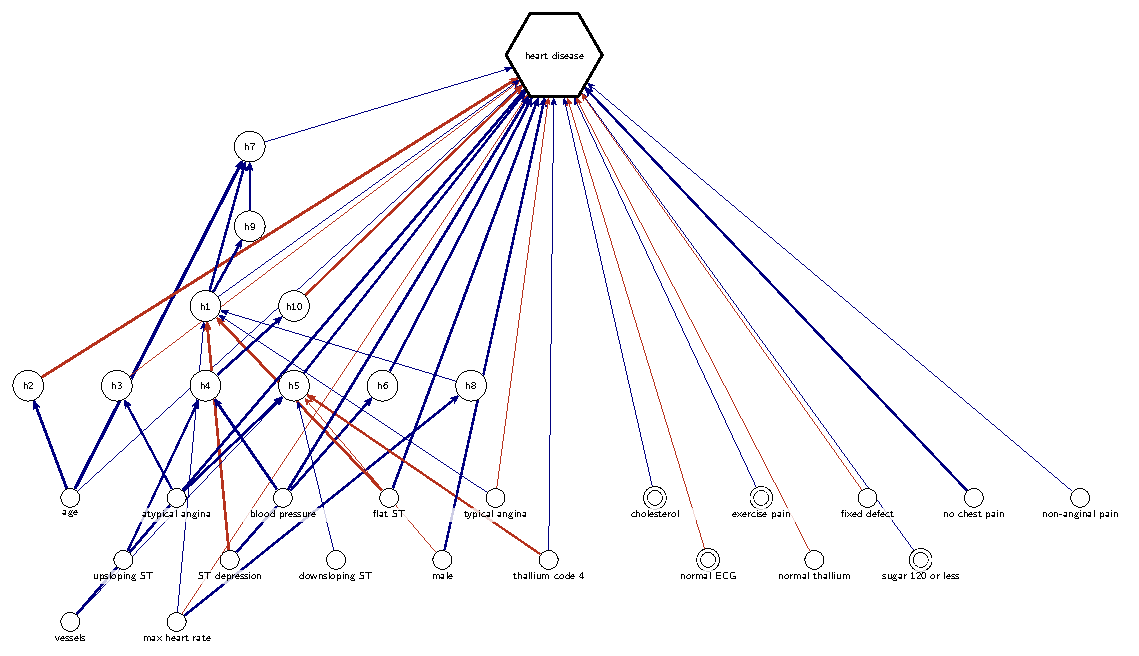
\includegraphics[width=\textheight,height=0.78\textwidth,keepaspectratio]{figures/exp2/networks/heart100-s3-raw}
  \caption{Heart-100, seed 3 (heart100-s3): the network as trained, before any explanation, in full. Inputs at the bottom (every input column its own node), hidden units by depth, the output at the top; 20 of 26 input columns are connected, with 10 hidden units and 45 enabled connections. Blue: positive weight (raises the score); red: negative weight (lowers it); thicker: larger weight. Orange outline and up arrow: raises the final prediction; teal and down arrow: lowers it; grey and double arrow: depends. Not used (no connection; 6 columns): female, sugar above 120, ST-T abnormal ECG, LVH on ECG, no exercise pain and reversible defect.}
  \label{fig:exp2-net-heart100-s3-raw}
\end{sidewaysfigure}

\clearpage
% Generated by thesis/ch7/exp2/networks.py -- do not edit by hand.
\begin{sidewaysfigure}
  \centering
  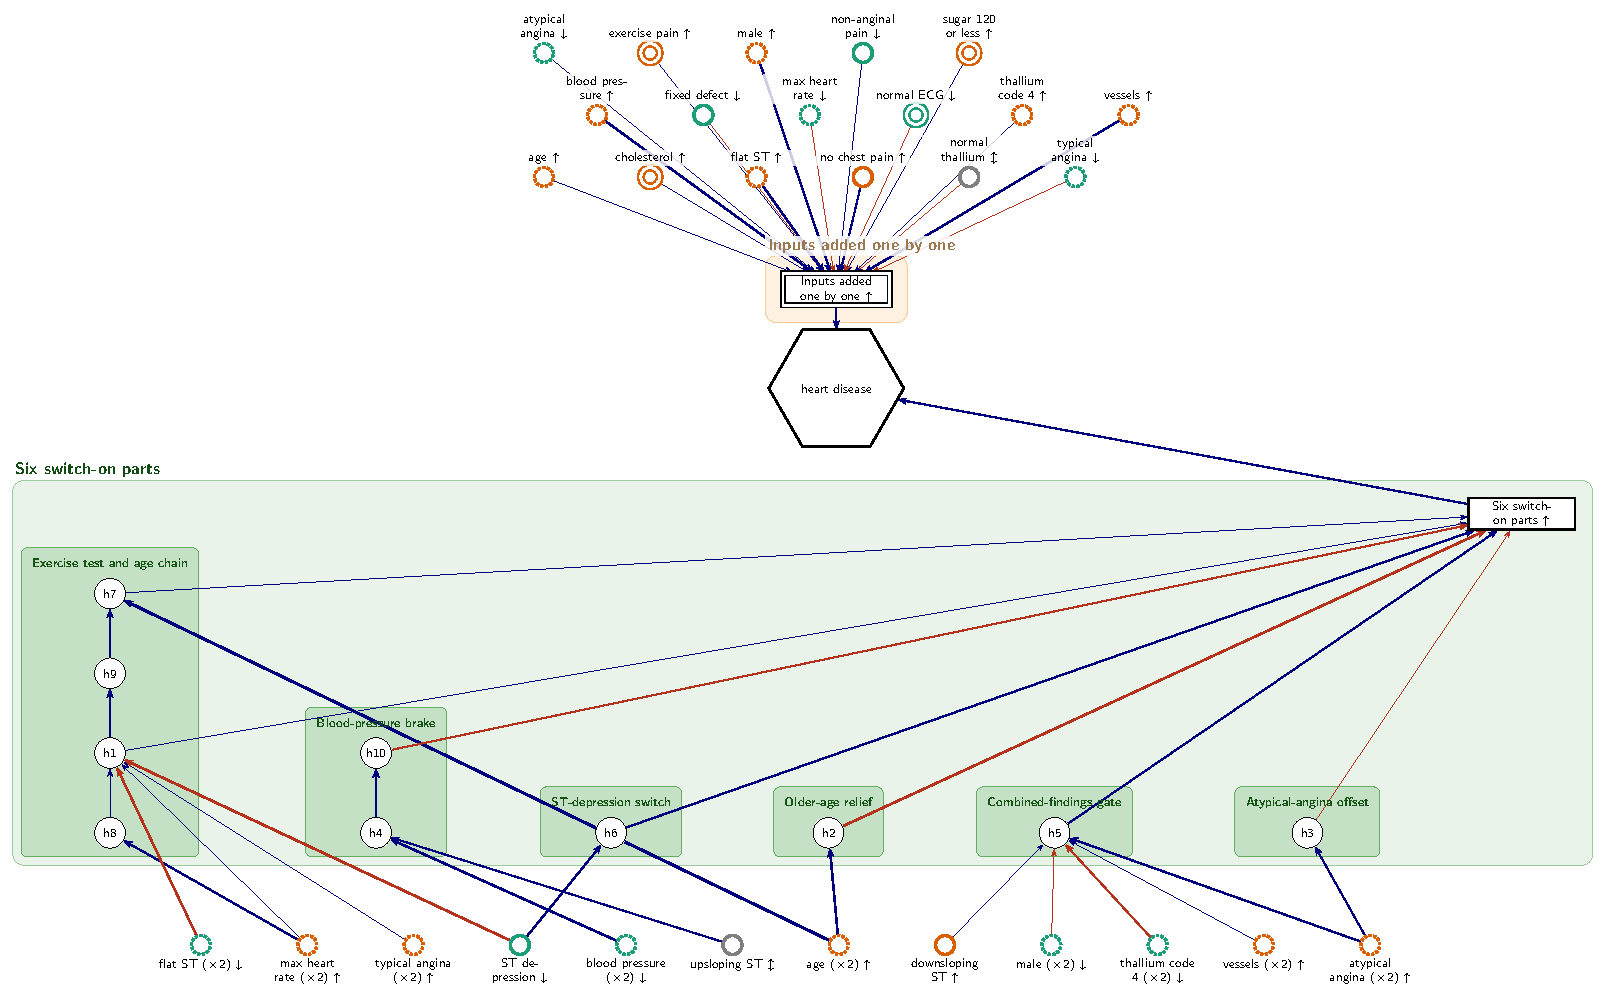
\includegraphics[width=\textheight,height=0.78\textwidth,keepaspectratio]{figures/exp2/networks/heart100-s3-explained}
  \caption{Heart-100, seed 3 (heart100-s3): every unit and connection of the explained model, nested by part. Shaded clusters are the 9 parts of the agent's explanation (7 leaf and 2 composition annotations, after 10 node splits and 2 identity nodes) and darker boxes the parts inside them; circles are hidden units; each cluster's rectangle is its output, a dashed `sum' an addition the next unit does; the hexagon is the model's output. An input used by several parts is drawn under each of them (dotted outline). Blue: positive weight (raises the score); red: negative weight (lowers it); thicker: larger weight. Orange outline and up arrow: raises the final prediction; teal and down arrow: lowers it; grey and double arrow: depends.}
  \label{fig:exp2-net-heart100-s3-explained}
\end{sidewaysfigure}

\clearpage
% Generated by thesis/ch7/exp2/networks.py -- do not edit by hand.
\begin{sidewaysfigure}
  \centering
  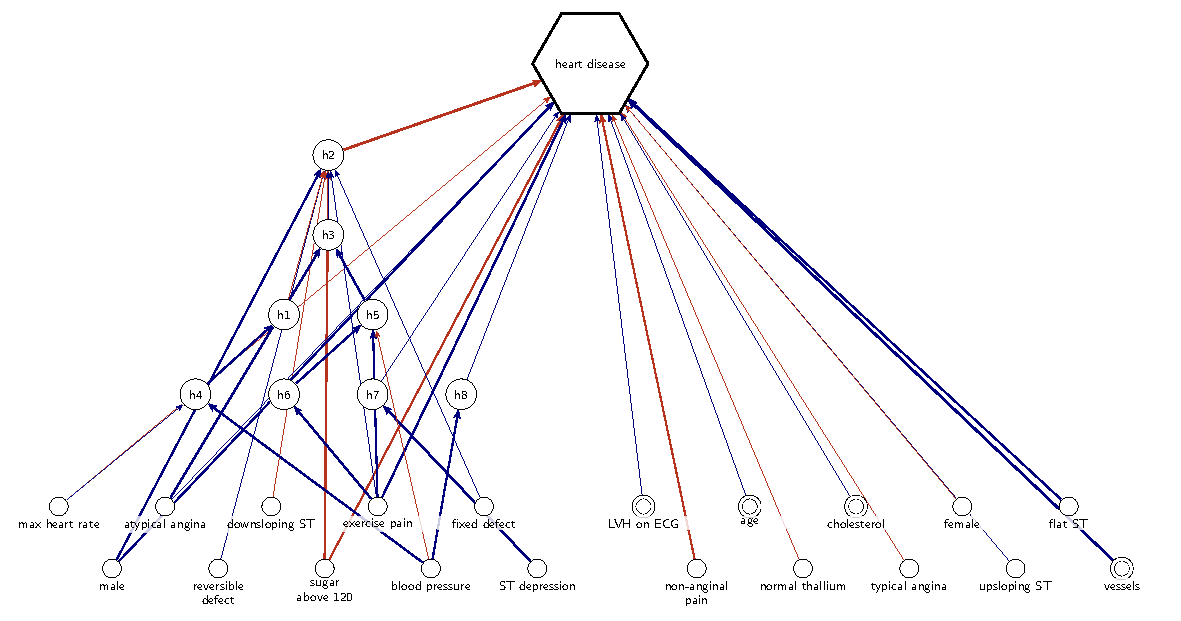
\includegraphics[width=\textheight,height=0.78\textwidth,keepaspectratio]{figures/exp2/networks/heart100-s4-raw}
  \caption{Heart-100, seed 4 (heart100-s4): the network as trained, before any explanation, in full. Inputs at the bottom (every input column its own node), hidden units by depth, the output at the top; 20 of 26 input columns are connected, with 8 hidden units and 37 enabled connections. Blue: positive weight (raises the score); red: negative weight (lowers it); thicker: larger weight. Orange outline and up arrow: raises the final prediction; teal and down arrow: lowers it; grey and double arrow: depends. Not used (no connection; 6 columns): no chest pain, sugar 120 or less, normal ECG, ST-T abnormal ECG, no exercise pain and thallium code 4.}
  \label{fig:exp2-net-heart100-s4-raw}
\end{sidewaysfigure}

\clearpage
% Generated by thesis/ch7/exp2/networks.py -- do not edit by hand.
\begin{sidewaysfigure}
  \centering
  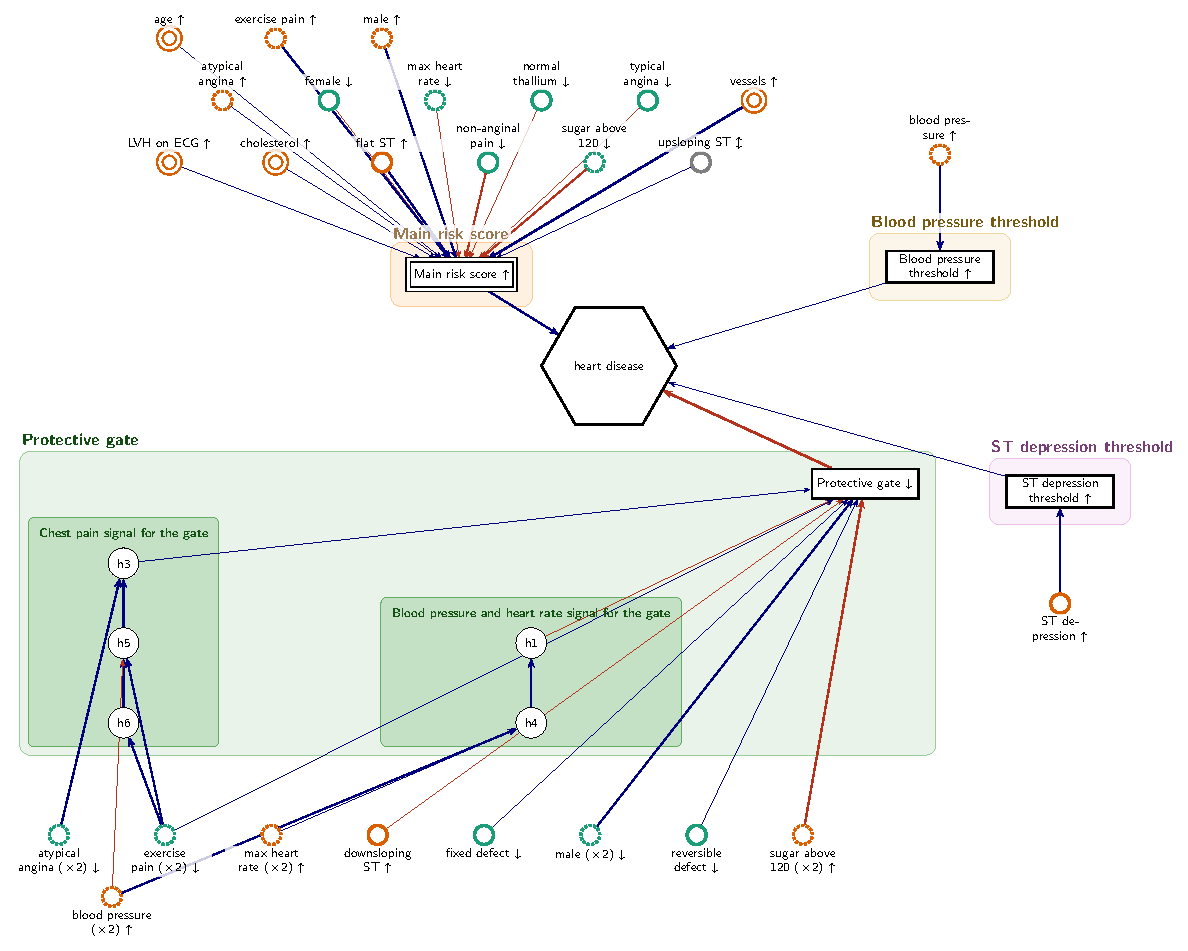
\includegraphics[width=\textheight,height=0.9\textwidth,keepaspectratio]{figures/exp2/networks/heart100-s4-explained}
  \caption{Heart-100, seed 4: the explained network, every unit nested by part.}
  \label{fig:exp2-net-heart100-s4-explained}
\end{sidewaysfigure}

\clearpage
% Generated by thesis/ch7/exp2/networks.py -- do not edit by hand.
\begin{sidewaysfigure}
  \centering
  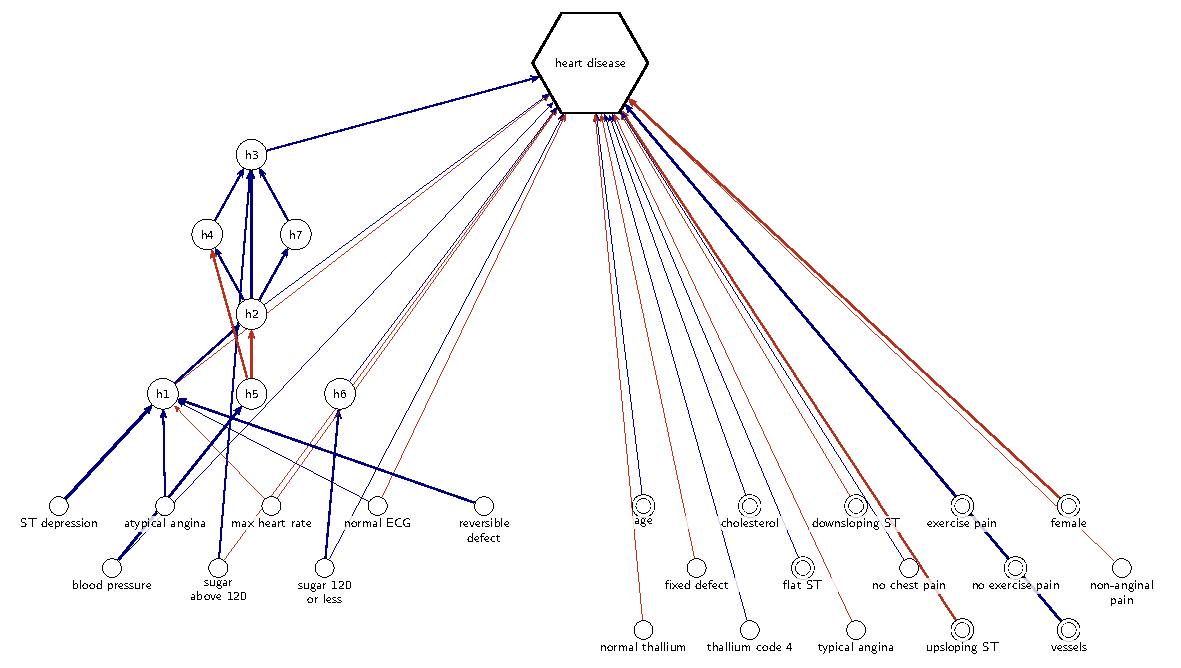
\includegraphics[width=\textheight,height=0.78\textwidth,keepaspectratio]{figures/exp2/networks/heart100-s5-raw}
  \caption{Heart-100, seed 5 (heart100-s5): the network as trained, before any explanation, in full. Inputs at the bottom (every input column its own node), hidden units by depth, the output at the top; 23 of 26 input columns are connected, with 7 hidden units and 40 enabled connections. Blue: positive weight (raises the score); red: negative weight (lowers it); thicker: larger weight. Orange outline and up arrow: raises the final prediction; teal and down arrow: lowers it; grey and double arrow: depends. Not used (no connection; 3 columns): male, ST-T abnormal ECG and LVH on ECG.}
  \label{fig:exp2-net-heart100-s5-raw}
\end{sidewaysfigure}

\clearpage
% Generated by thesis/ch7/exp2/networks.py -- do not edit by hand.
\begin{sidewaysfigure}
  \centering
  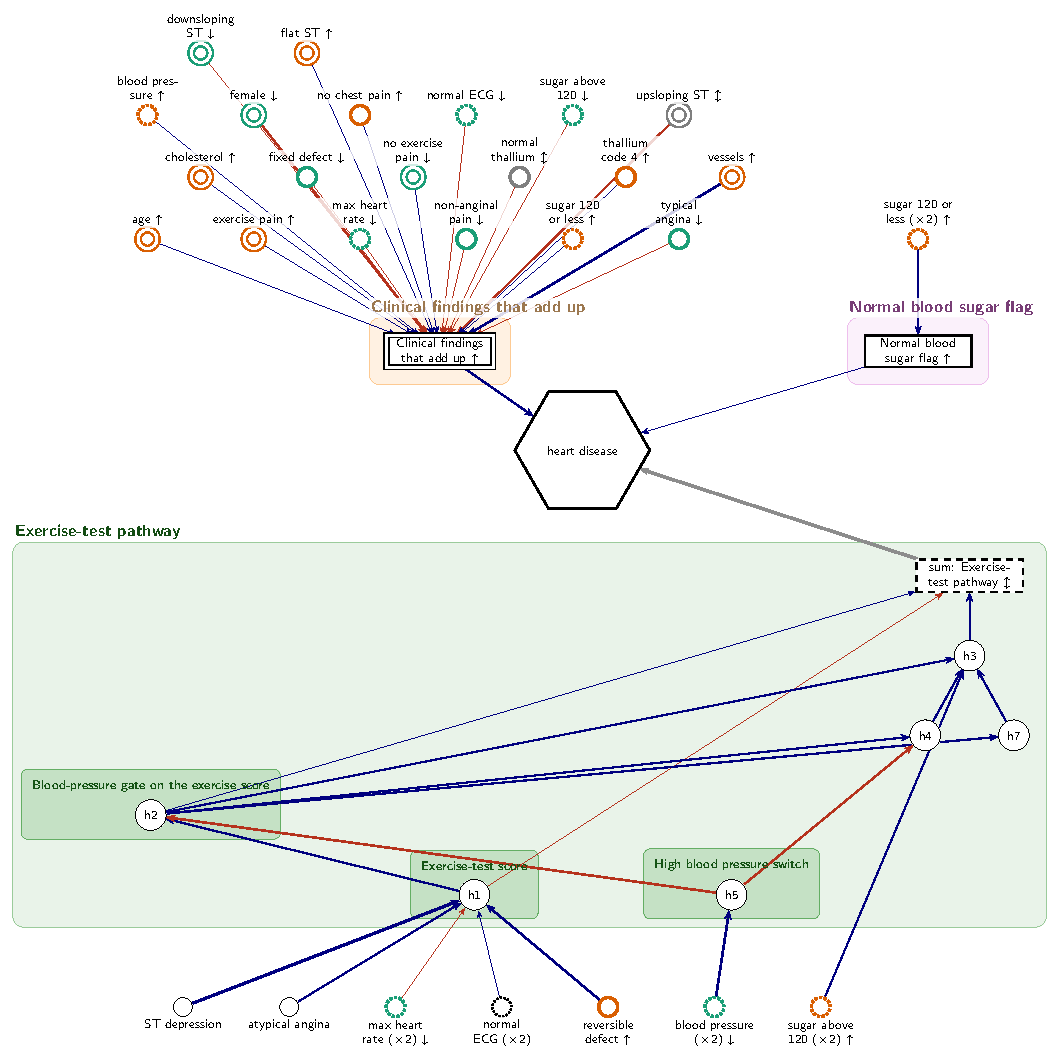
\includegraphics[width=\textheight,height=0.78\textwidth,keepaspectratio]{figures/exp2/networks/heart100-s5-explained}
  \caption{Heart-100, seed 5 (heart100-s5): every unit and connection of the explained model, nested by part. Shaded clusters are the 7 parts of the agent's explanation (4 leaf and 3 composition annotations, after 5 node splits and 1 identity nodes) and darker boxes the parts inside them; circles are hidden units; each cluster's rectangle is its output, a dashed `sum' an addition the next unit does; the hexagon is the model's output. An input used by several parts is drawn under each of them (dotted outline). Blue: positive weight (raises the score); red: negative weight (lowers it); thicker: larger weight. Orange outline and up arrow: raises the final prediction; teal and down arrow: lowers it; grey and double arrow: depends.}
  \label{fig:exp2-net-heart100-s5-explained}
\end{sidewaysfigure}

\clearpage
% Generated by thesis/ch7/exp2/networks.py -- do not edit by hand.
\ifdefined\netfigheight\else\newlength{\netfigheight}\setlength{\netfigheight}{0.9\textwidth}\fi
\begin{sidewaysfigure}
  \centering
  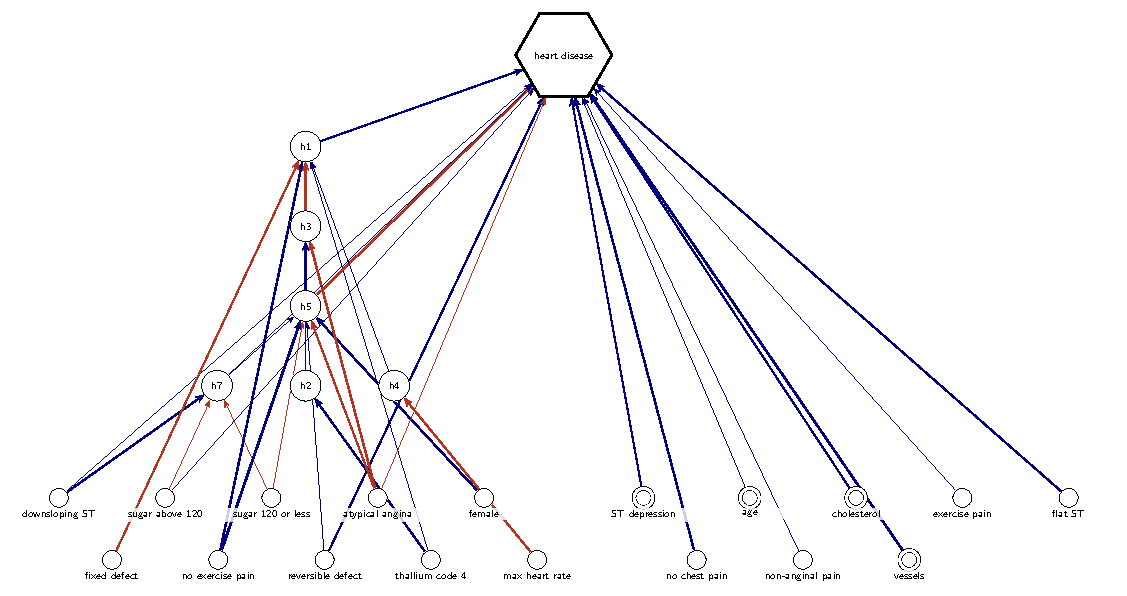
\includegraphics[width=\textheight,height=\netfigheight,keepaspectratio]{figures/exp2/networks/heart100-s6-raw}
  \caption{Heart-100, seed 6: the network as trained, before any explanation.}
  \label{fig:exp2-net-heart100-s6-raw}
\end{sidewaysfigure}

\clearpage
% Generated by thesis/ch7/exp2/networks.py -- do not edit by hand.
\ifdefined\netfigheight\else\newlength{\netfigheight}\setlength{\netfigheight}{0.9\textwidth}\fi
\begin{sidewaysfigure}
  \centering
  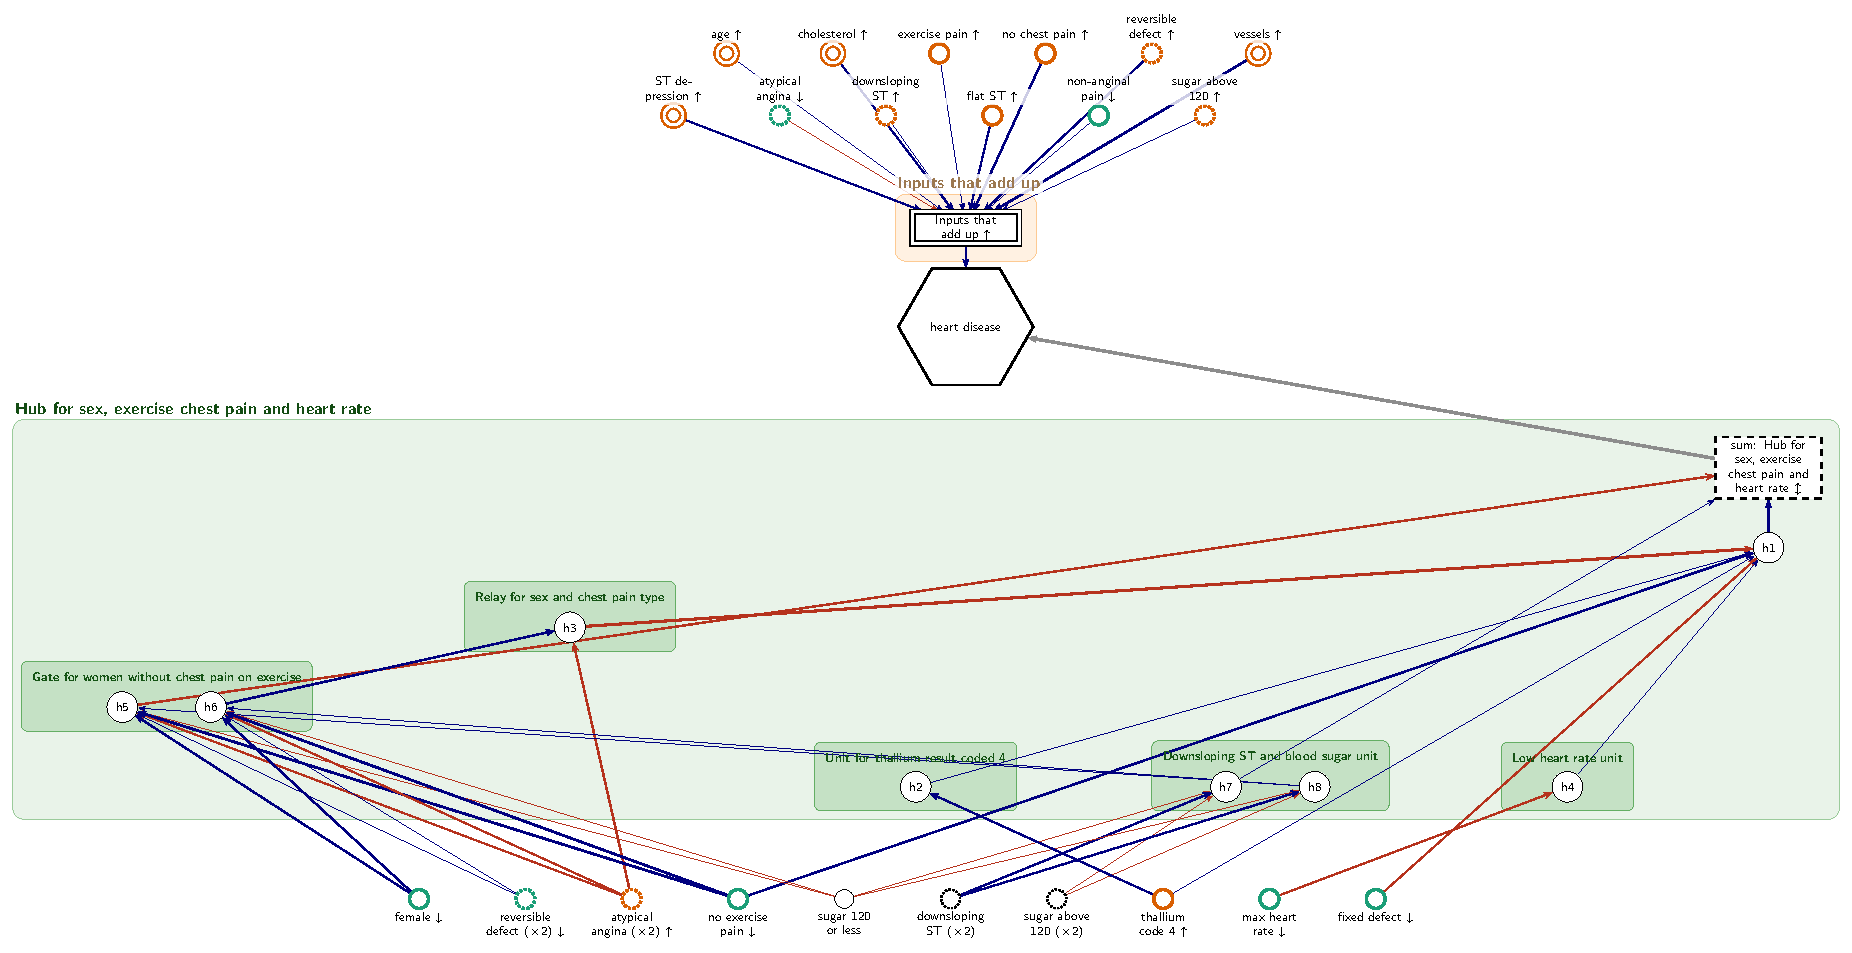
\includegraphics[width=\textheight,height=\netfigheight,keepaspectratio]{figures/exp2/networks/heart100-s6-explained}
  \caption{Heart-100, seed 6: the explained network, every unit nested by part.}
  \label{fig:exp2-net-heart100-s6-explained}
\end{sidewaysfigure}

\clearpage
% Generated by thesis/ch7/exp2/networks.py -- do not edit by hand.
\begin{sidewaysfigure}
  \centering
  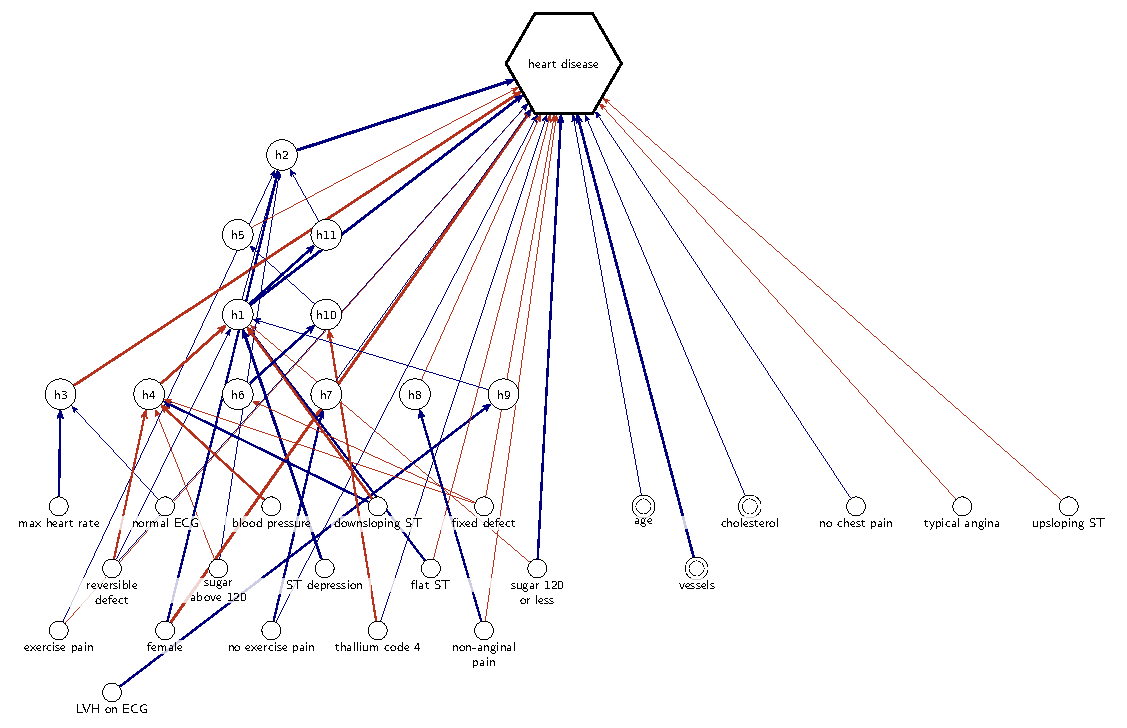
\includegraphics[width=\textheight,height=0.9\textwidth,keepaspectratio]{figures/exp2/networks/heart100-s7-raw}
  \caption{Heart-100, seed 7: the network as trained, before any explanation.}
  \label{fig:exp2-net-heart100-s7-raw}
\end{sidewaysfigure}

\clearpage
% Generated by thesis/ch7/exp2/networks.py -- do not edit by hand.
\begin{sidewaysfigure}
  \centering
  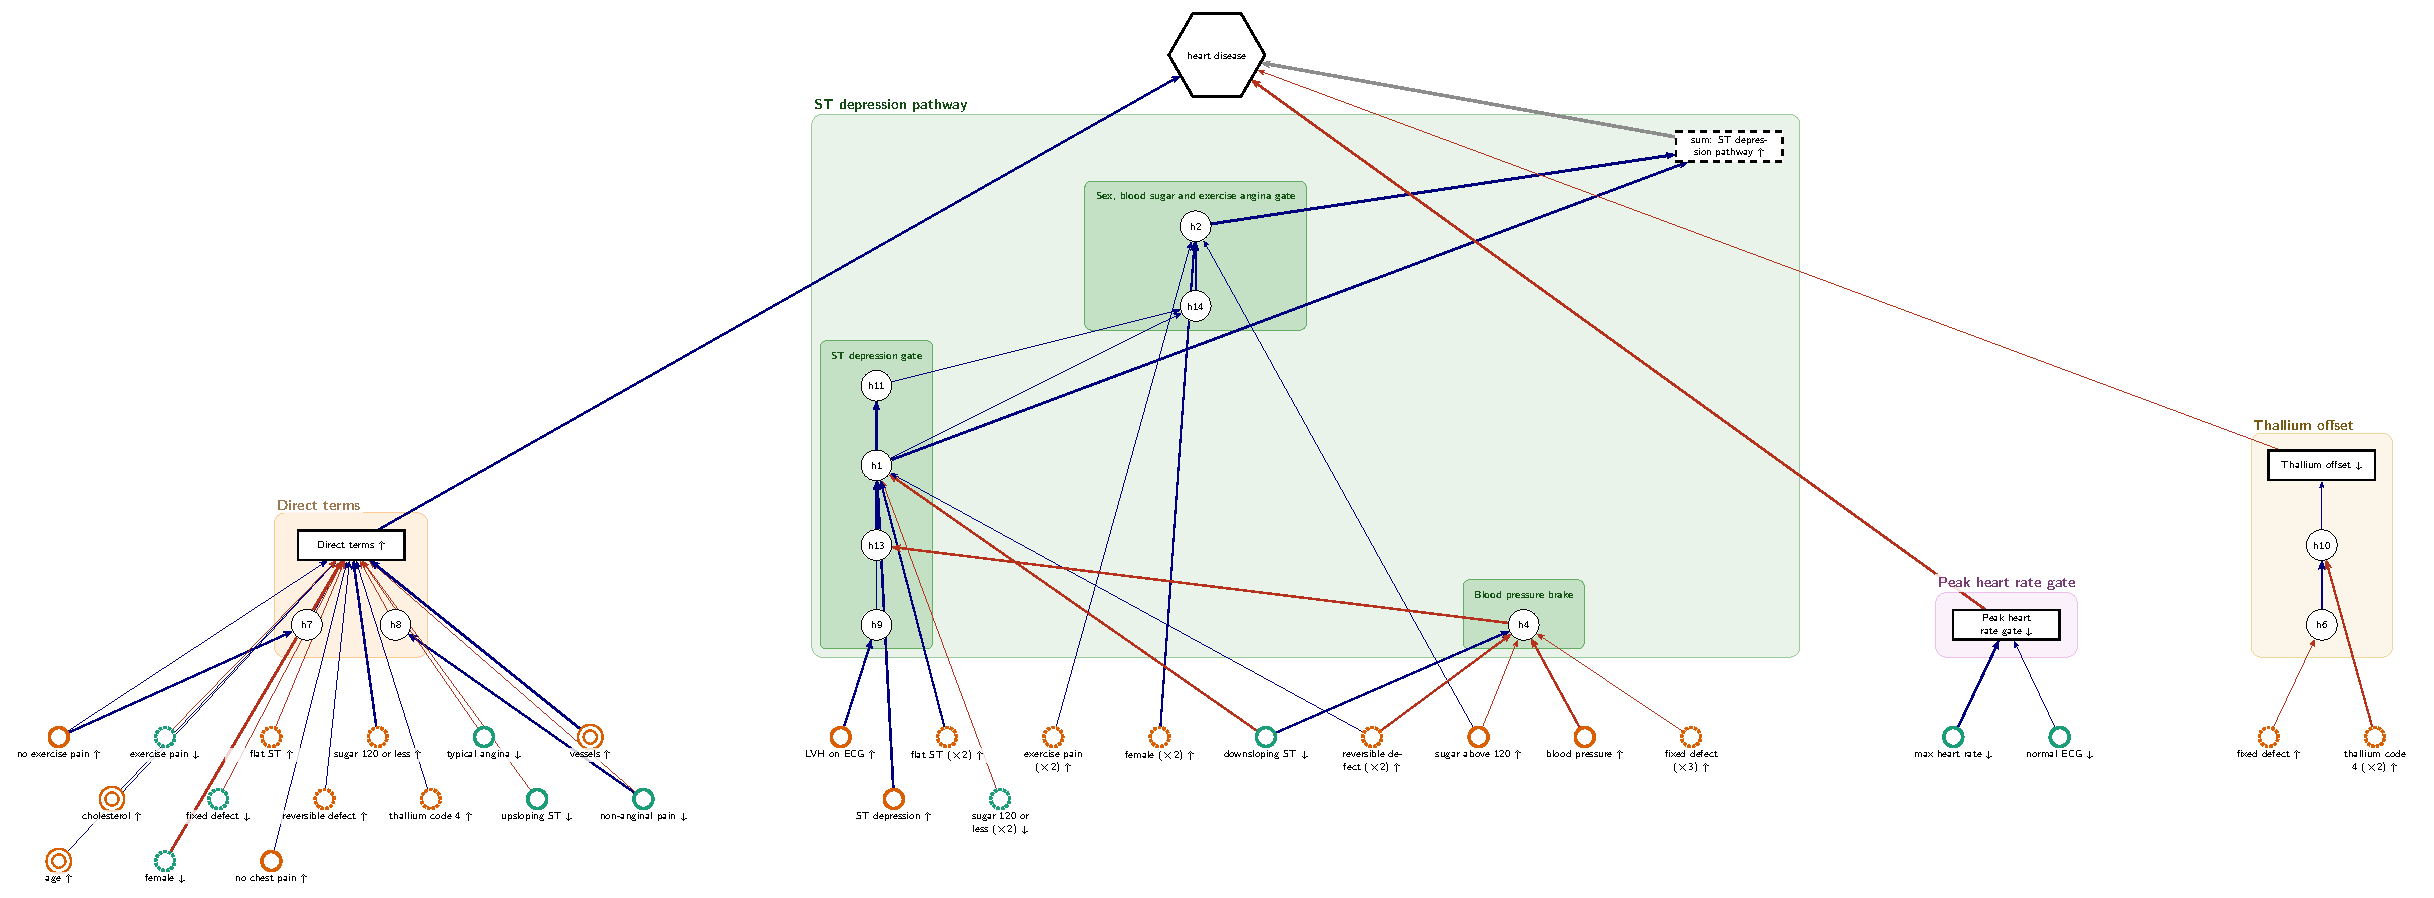
\includegraphics[trim={0.0bp 0 572.1bp 0},clip,width=\textheight,height=0.78\textwidth,keepaspectratio]{figures/exp2/networks/heart100-s7-explained}
  \caption{Heart-100, seed 7 (heart100-s7): every unit and connection of the explained model, nested by part. Shaded clusters are the 8 parts of the agent's explanation (6 leaf and 2 composition annotations, after 9 node splits and 3 identity nodes) and darker boxes the parts inside them; circles are hidden units; each cluster's rectangle is its output, a dashed `sum' an addition the next unit does; the hexagon is the model's output. An input used by several parts is drawn under each of them (dotted outline). Blue: positive weight (raises the score); red: negative weight (lowers it); thicker: larger weight. Orange outline and up arrow: raises the final prediction; teal and down arrow: lowers it; grey and double arrow: depends. Drawn in 2 pieces, left to right, on this and the next page.}
  \label{fig:exp2-net-heart100-s7-explained}
\end{sidewaysfigure}
\clearpage
\begin{sidewaysfigure}
  \centering
  \ContinuedFloat
  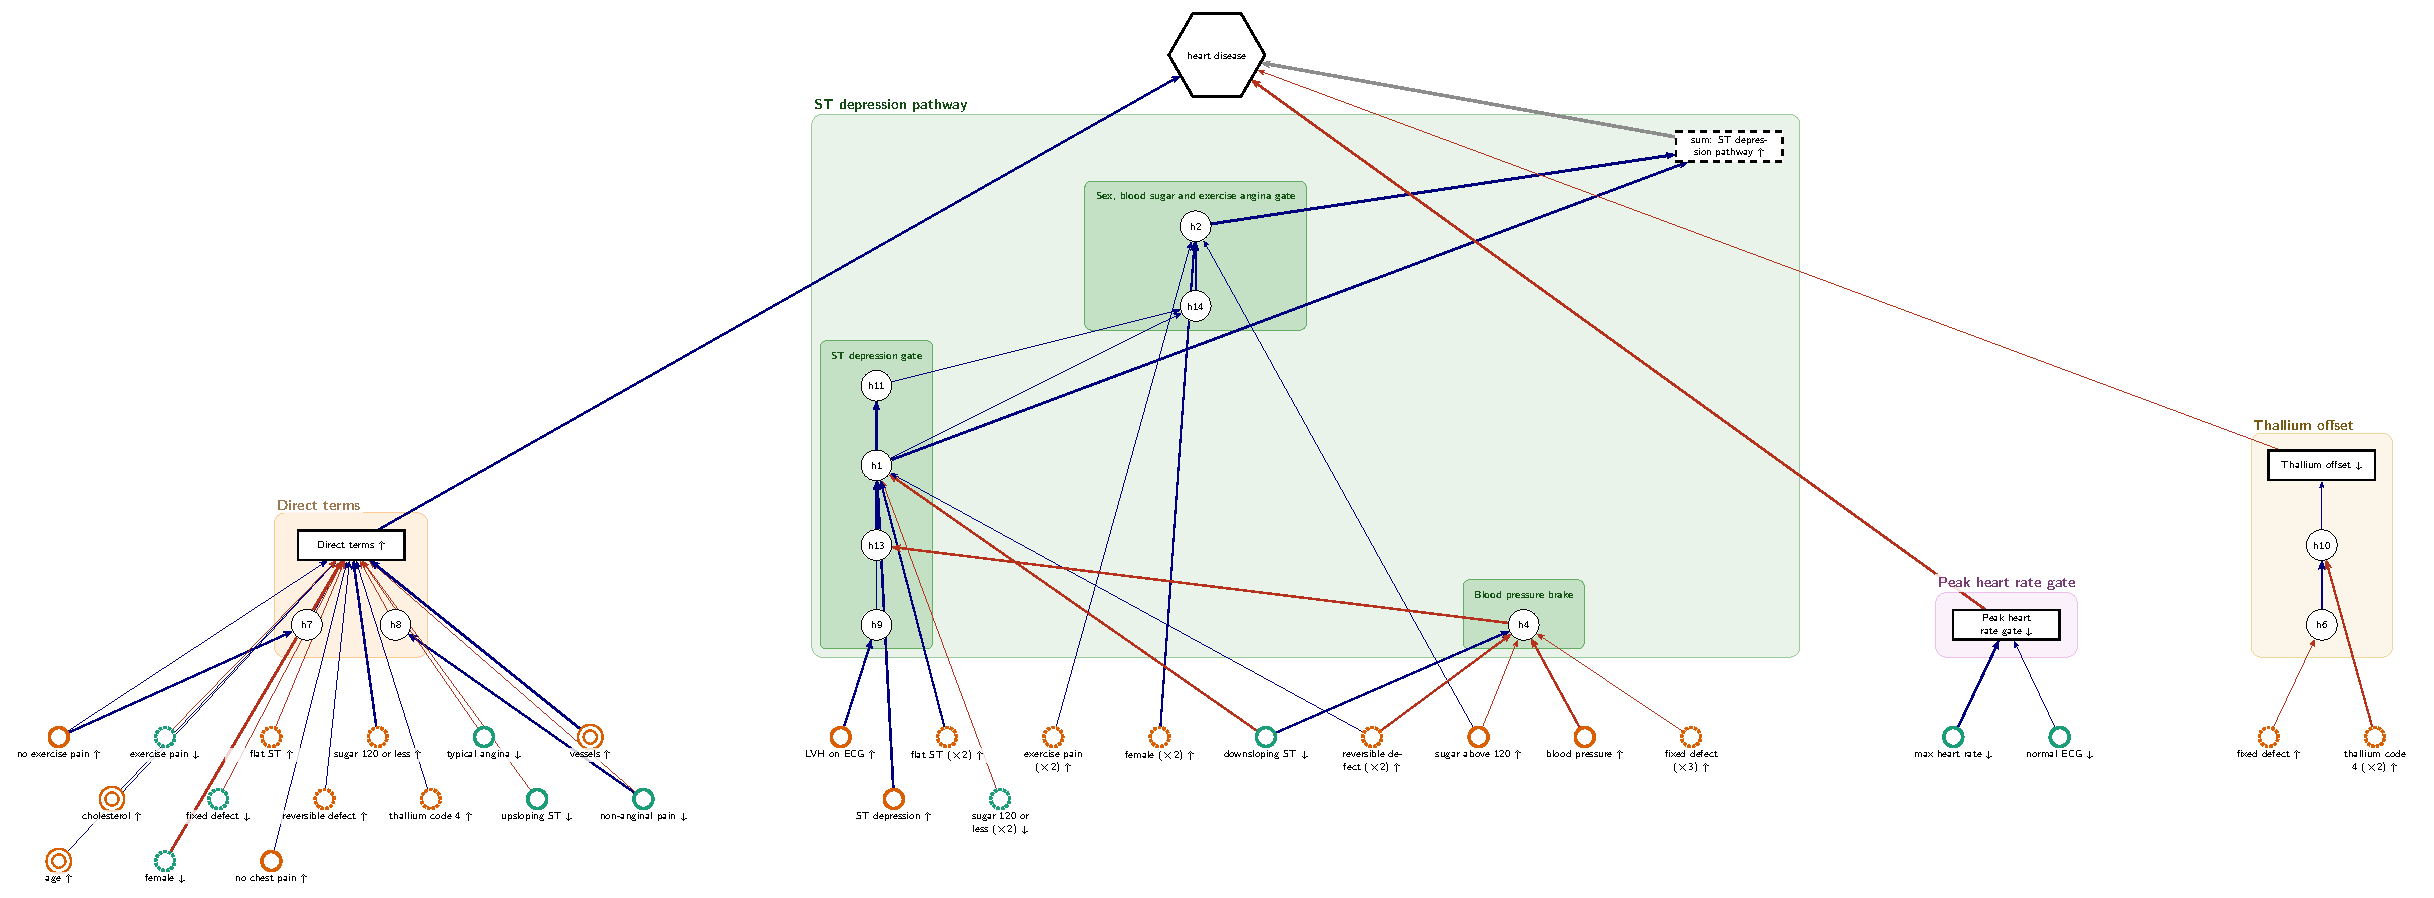
\includegraphics[trim={572.1bp 0 0.0bp 0},clip,width=\textheight,height=0.78\textwidth,keepaspectratio]{figures/exp2/networks/heart100-s7-explained}
  \caption[]{(continued, piece 2 of 2).}
\end{sidewaysfigure}

\clearpage
% Generated by thesis/ch7/exp2/networks.py -- do not edit by hand.
\begin{sidewaysfigure}
  \centering
  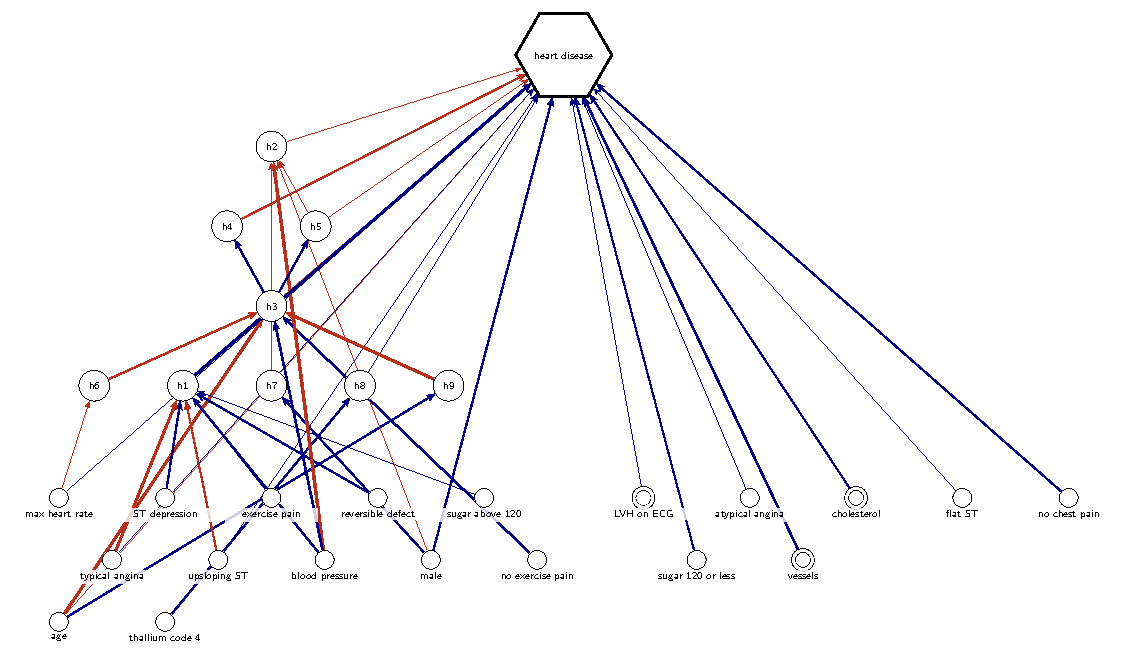
\includegraphics[width=\textheight,height=0.78\textwidth,keepaspectratio]{figures/exp2/networks/heart100-s8-raw}
  \caption{Heart-100, seed 8 (heart100-s8): the network as trained, before any explanation, in full. Inputs at the bottom (every input column its own node), hidden units by depth, the output at the top; 19 of 26 input columns are connected, with 9 hidden units and 40 enabled connections. Blue: positive weight (raises the score); red: negative weight (lowers it); thicker: larger weight. Orange outline and up arrow: raises the final prediction; teal and down arrow: lowers it; grey and double arrow: depends. Not used (no connection; 7 columns): female, non-anginal pain, normal ECG, ST-T abnormal ECG, downsloping ST, normal thallium and fixed defect.}
  \label{fig:exp2-net-heart100-s8-raw}
\end{sidewaysfigure}

\clearpage
% Generated by thesis/ch7/exp2/networks.py -- do not edit by hand.
\begin{sidewaysfigure}
  \centering
  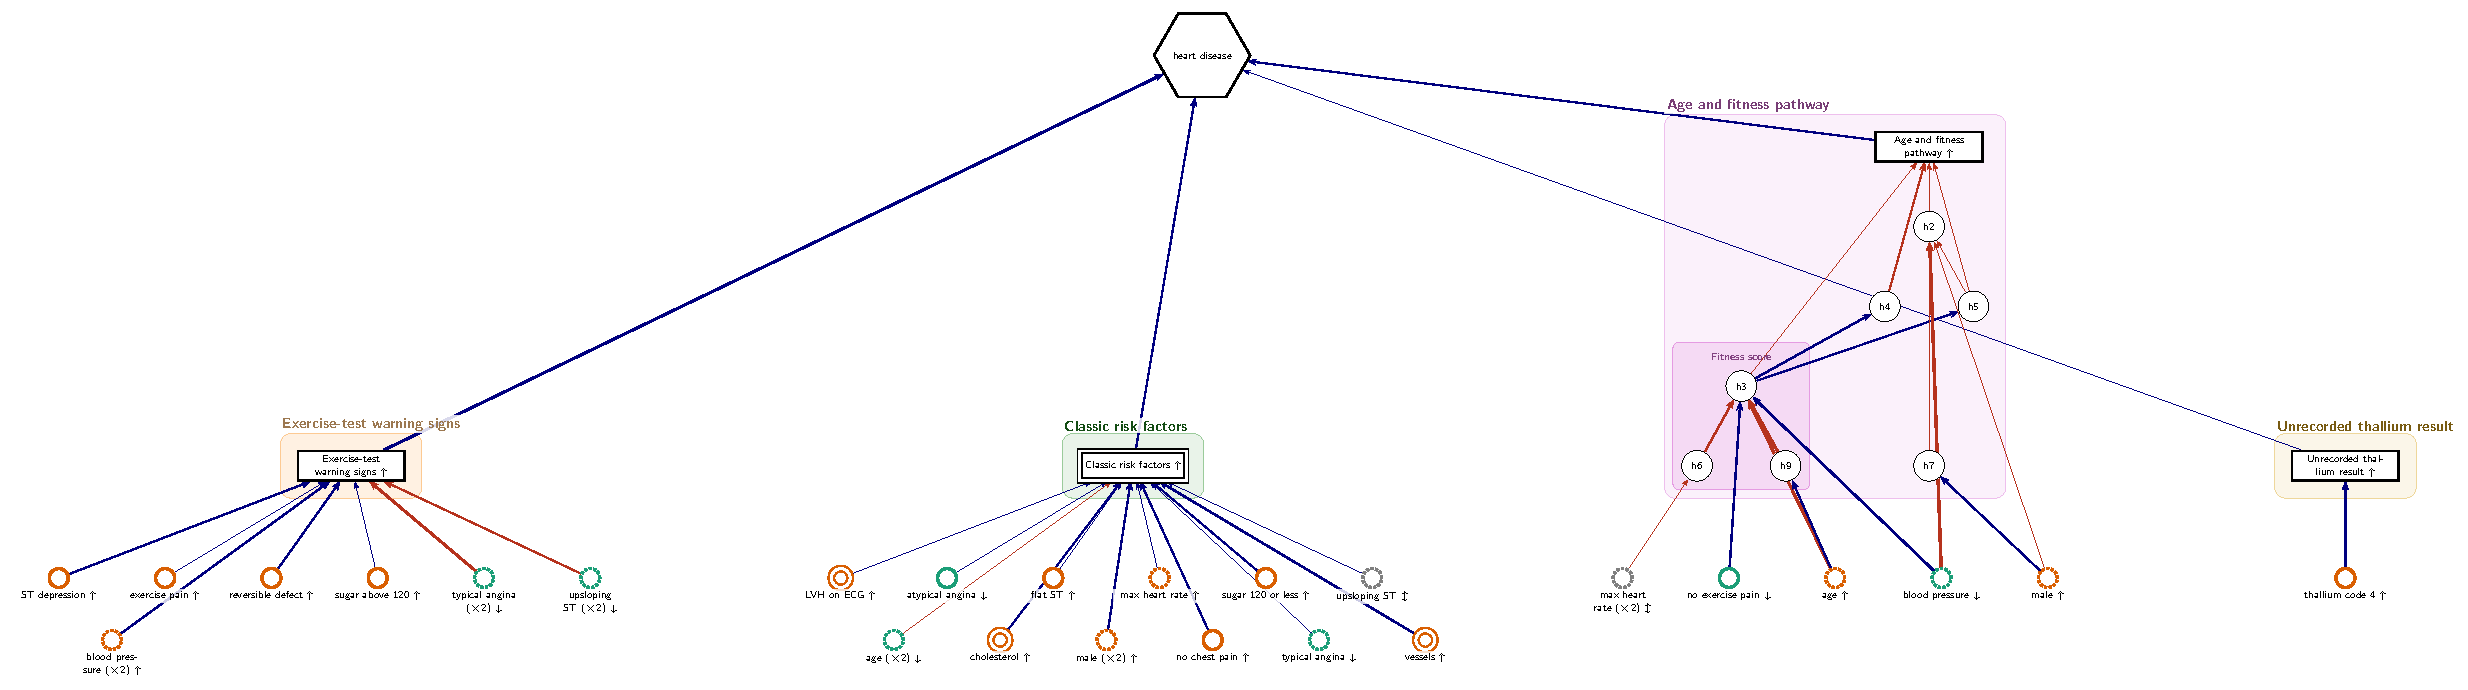
\includegraphics[width=\textheight,height=0.9\textwidth,keepaspectratio]{figures/exp2/networks/heart100-s8-explained}
  \caption{Heart-100, seed 8: the explained network, every unit nested by part.}
  \label{fig:exp2-net-heart100-s8-explained}
\end{sidewaysfigure}

\clearpage
% Generated by thesis/ch7/exp2/networks.py -- do not edit by hand.
\begin{sidewaysfigure}
  \centering
  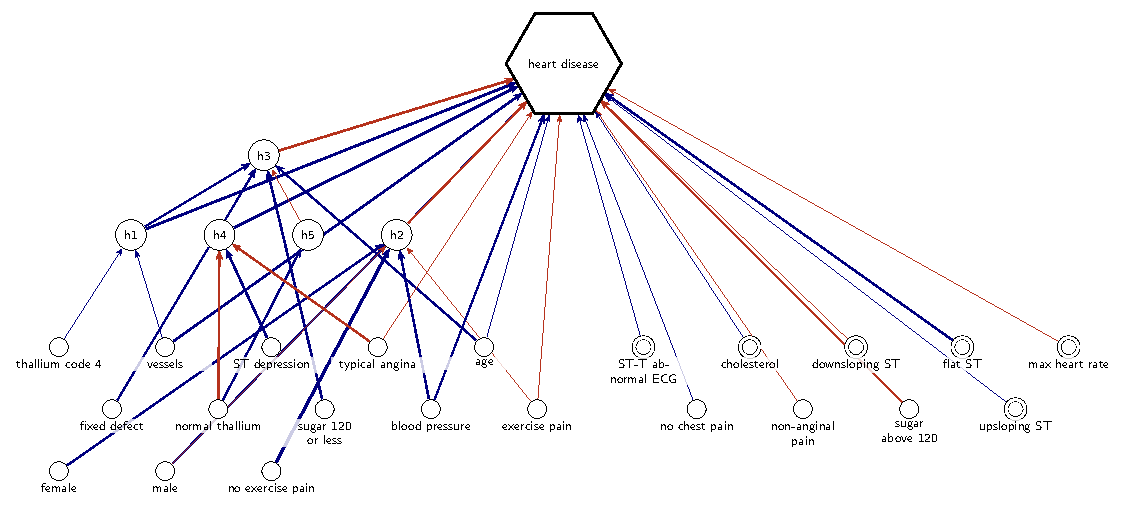
\includegraphics[width=\textheight,height=0.9\textwidth,keepaspectratio]{figures/exp2/networks/heart100-s9-raw}
  \caption{Heart-100, seed 9: the network as trained, before any explanation.}
  \label{fig:exp2-net-heart100-s9-raw}
\end{sidewaysfigure}

\clearpage
% Generated by thesis/ch7/exp2/networks.py -- do not edit by hand.
\begin{sidewaysfigure}
  \centering
  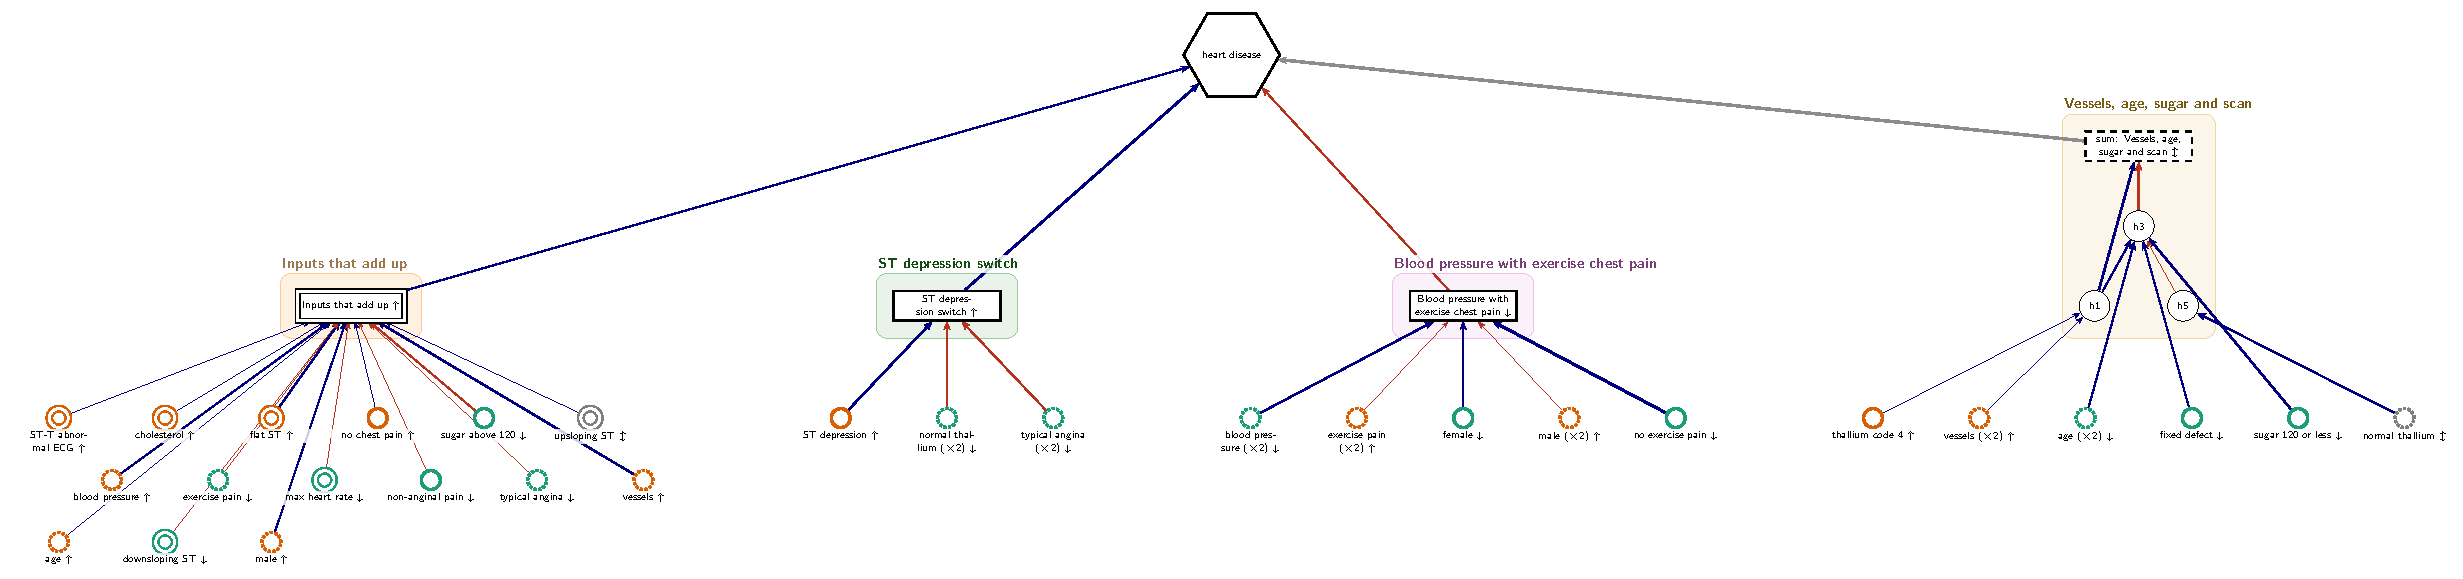
\includegraphics[trim={0.0bp 0 579.2bp 0},clip,width=\textheight,height=0.78\textwidth,keepaspectratio]{figures/exp2/networks/heart100-s9-explained}
  \caption{Heart-100, seed 9 (heart100-s9): every unit and connection of the explained model, nested by part. Shaded clusters are the 5 parts of the agent's explanation (4 leaf and 1 composition annotations, after 7 node splits and 1 identity nodes) and darker boxes the parts inside them; circles are hidden units; each cluster's rectangle is its output, a dashed `sum' an addition the next unit does; the hexagon is the model's output. An input used by several parts is drawn under each of them (dotted outline). Blue: positive weight (raises the score); red: negative weight (lowers it); thicker: larger weight. Orange outline and up arrow: raises the final prediction; teal and down arrow: lowers it; grey and double arrow: depends. Drawn in 2 pieces, left to right, on this and the next page.}
  \label{fig:exp2-net-heart100-s9-explained}
\end{sidewaysfigure}
\clearpage
\begin{sidewaysfigure}
  \centering
  \ContinuedFloat
  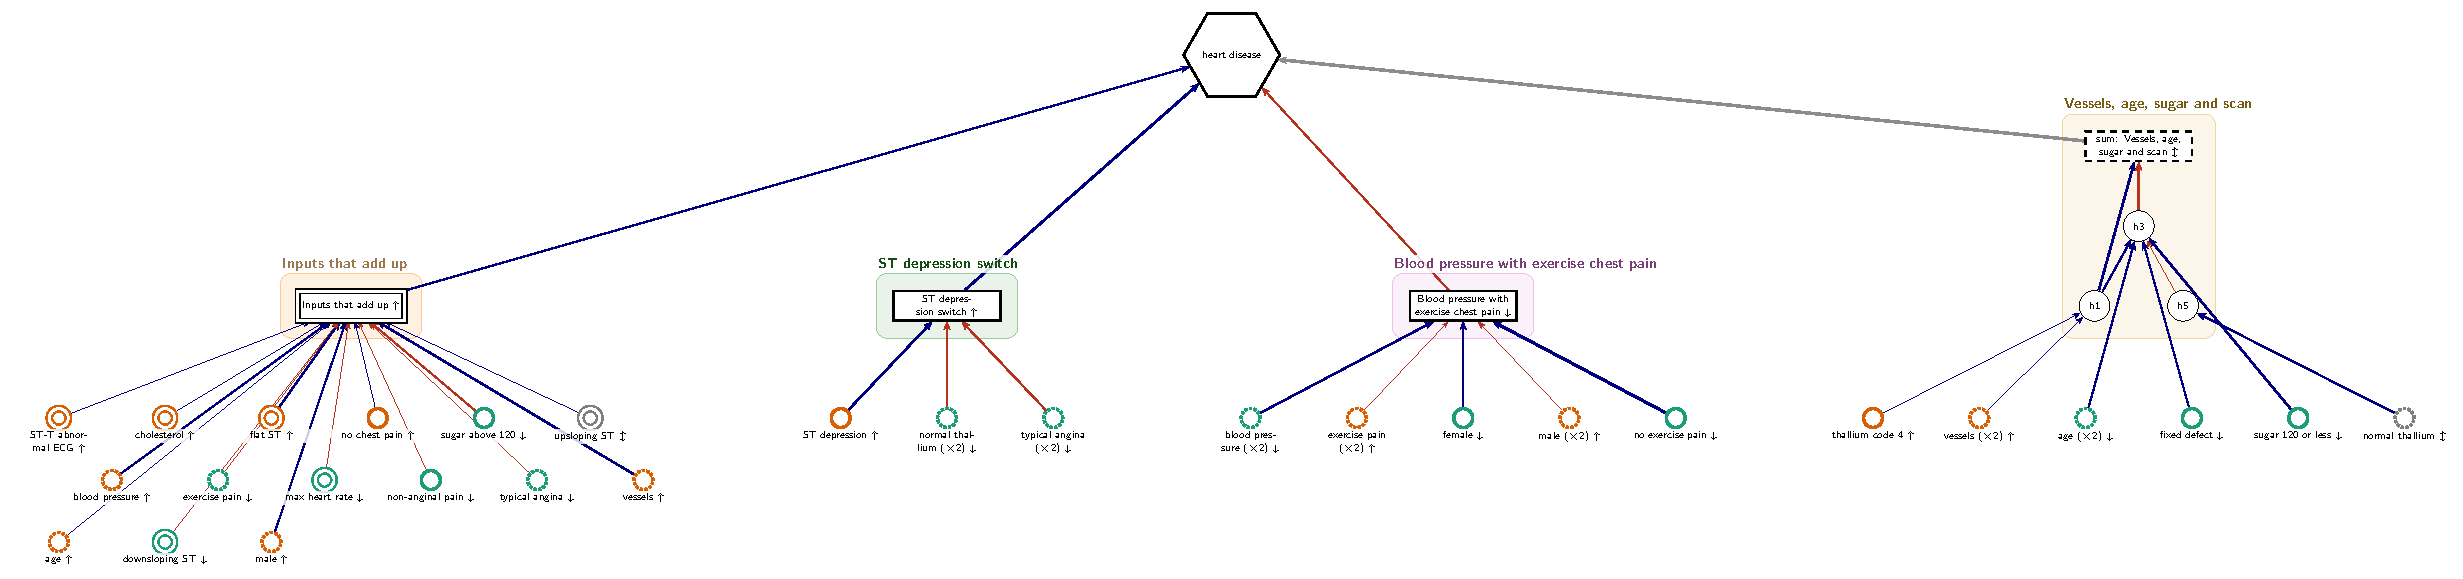
\includegraphics[trim={579.2bp 0 0.0bp 0},clip,width=\textheight,height=0.78\textwidth,keepaspectratio]{figures/exp2/networks/heart100-s9-explained}
  \caption[]{(continued, piece 2 of 2).}
\end{sidewaysfigure}

\clearpage
